\special{pdf:minorversion 7}
\PassOptionsToPackage{dvipsnames}{xcolor}
\documentclass[12pt,letterpaper,twoside]{report}

\usepackage[todonotes={textsize=scriptsize}, final]{changes}
\usepackage[left=1in, right=1in, top=1in, bottom=1in]{geometry}
\usepackage{setspace}
\usepackage{layout}
\usepackage{parskip}
\usepackage{amsmath}
\usepackage{amssymb}
\usepackage[T1]{fontenc}
\usepackage{fontspec}
\setmainfont{XCharter}
\usepackage{unicode-math}
\setmathfont{XCharter-Math.otf}
\setsansfont{IBMPlexSans}[
    Extension = .otf,
    UprightFont = *-Regular,
    BoldFont = *-SemiBold,
    ItalicFont = *-Italic,
    BoldItalicFont = *-SemiBoldItalic,
    Scale = MatchLowercase
]
\setmonofont{IBMPlexMono}[Scale=MatchLowercase]
\usepackage{multicol}
\usepackage{multirow}
\usepackage{pdfpages}
\usepackage{pdflscape}
\usepackage{afterpage}
\usepackage{graphicx}
% \DeclareGraphicsExtensions{.png,.pdf}
\DeclareGraphicsExtensions{.pdf,.png}
\usepackage{tabularx}
% \usepackage{expl3}
% \usepackage{calc}
\usepackage[version=4]{mhchem}
\usepackage{siunitx}
\usepackage{bm}
\usepackage[dvipsnames]{xcolor}
\usepackage{caption}
\usepackage{subcaption}
\usepackage[sf,bf]{titlesec}
\usepackage{colortbl}
\usepackage{enumitem}
\usepackage{listings}
\usepackage{booktabs}
\usepackage{gensymb}
\usepackage[font=itshape]{quoting}
\usepackage{wrapfig}
\usepackage{fancyhdr}
\usepackage{lipsum}
\usepackage[final]{draftwatermark}
\usepackage{soul}
\usepackage[
    style=ieee,
    citestyle=numeric-comp,
    urldate=iso]{biblatex}
% \usepackage{datetime}
\usepackage{nameref}
\usepackage{hyperref}
\definecolor{McGillRed}{cmyk}{0, 1, 0.9, 0}
\hypersetup{
    colorlinks=true,
    linkcolor=cyan,
    anchorcolor=cyan,
    citecolor=cyan,
    filecolor=cyan,
    urlcolor=cyan
}
\setdeletedmarkup{\textcolor{McGillRed}{\sout{#1}}}
% \setdeletedmarkup{\textcolor{McGillRed}{#1}}
\definechangesauthor[color=violet, name={Emmanuel Duplay}]{ED}
\definechangesauthor[color=cyan, name={Barry Zandbergen}]{BZ}
\definechangesauthor[color=McGillRed, name={Andrew Higgins}]{AH}

% \input{titlesec.tex}
\addbibresource{ref.bib}

\title{Working title}
\author{Gabriel Dubé}
\date{0000-00-00}

\renewcommand{\headrulewidth}{0pt}
\renewcommand{\chaptermark}[1]{\markboth{\MakeUppercase{\thechapter.\ #1}}{}}
\renewcommand{\sectionmark}[1]{\markright{\MakeUppercase{\thesection.\ #1}}}

\renewcommand{\chapterautorefname}{Chapter}
\renewcommand{\sectionautorefname}{Section}

\newcommand{\shotsettings}[4]{\texttt{#1}: #2~ms, \textit{f}/#3, ND#4}

\newcommand{\dd}[2]{\frac{\mathrm{d}#1}{\mathrm{d}#2}}
\newcommand{\ddi}[2]{\mathrm{d}#1/\mathrm{d}#2}

\newcommand{\blankpage}{%
    \null
    \thispagestyle{empty}%
    \addtocounter{page}{-1}%
    \newpage}

% Track changes commands
% \newcommand{\change}[1]{\textcolor{McGillRed}{#1}}
% \newenvironment{changeblock}{\color{McGillRed}}{}
% \renewcommand{\change}[1]{#1}  % Comment out to suppress changes
% \renewenvironment{changeblock}{}{}  % Comment out to suppress changes

\fancypagestyle{fancy}{
    \fancyhf{}
    \fancyhfinit{\sffamily}
    \lhead{\leftmark}
    \rhead{\rightmark}
    % \lfoot{AE5050}
    % \rfoot{\thepage}
    \fancyfoot[LE,RO]{\thepage}
    \fancyfoot[RE,LO]{AE5050}
}

\fancypagestyle{plain}{
    \fancyhf{}
    \fancyfoot[C]{\sffamily \thepage}
    
}

\pagestyle{fancy}

\SetWatermarkText{\sffamily \textbf{DRAFT}}
\SetWatermarkFontSize{2cm}
\SetWatermarkColor[gray]{0.85}
    
\definecolor{bggray}{gray}{0.97}
\definecolor{txtgray}{gray}{0.3}

\lstdefinestyle{mystyle}{
    backgroundcolor=\color{bggray},   
    commentstyle=\color{MidnightBlue},
    keywordstyle=\color{Plum},
    numberstyle=\scriptsize\ttfamily\color{Gray},
    stringstyle=\color{RedOrange},
    % identifierstyle=\color{Turquoise},
    basicstyle=\ttfamily\color{txtgray},
    breakatwhitespace=false,         
    breaklines=true,                 
    captionpos=t,                    
    keepspaces=true,                 
    numbers=left,                    
    numbersep=5pt,                  
    showspaces=false,                
    showstringspaces=false,
    showtabs=false,                  
    tabsize=2
}

\lstset{style=mystyle}
\newenvironment{plainchp}[1]
    {
        \newgeometry{left=4.2cm,right=4.2cm}
        \fancypagestyle{abstractplain}{
            \fancyhf{}
            \fancyfootoffset[lh]{0pt}
            \fancyfoot[C]{\sffamily \thepage}  
        }
        \pagestyle{abstractplain}
        
        \phantomsection
        \begin{center}
            \sffamily \Large \caps{\textbf{\MakeUppercase{#1}}}
        \end{center}
        \vspace{0.2cm}
        \markboth{\MakeUppercase{#1}}{}
    }
    {
        \restoregeometry
        \pagestyle{fancy}
    }

\newenvironment{statement}[1]
    {
        \vspace{\parskip}
        \begin{center}\begin{minipage}{0.85\textwidth}
            {\sffamily \footnotesize \color{cyan}\caps{\MakeUppercase{#1}}}\\\itshape
    }
    {
        \end{minipage}\end{center}
        \vspace{\parskip}
    }

\sisetup{detect-all}

\begin{document}
    \setlength{\parindent}{0pt}
    \setlength{\headheight}{13.6pt}
    
\includepdf{assets/cover.pdf}
    \begin{titlepage}
    \thispagestyle{empty}
    % \centering
    \sffamily
    \vspace*{3cm}
    {\large \color{cyan}
        % Suptitle
        Master's Thesis
    }

    \vspace{0.3cm}
    \textbf{{\LARGE Design and Test of an Argon Laser-Plasma Thruster\\Laboratory Model}}

    \vspace{0.2cm}
    {\large 
        % Subtitle
        Submitted to fulfill the requirements of the degree of Master of Science at\\the Delft University of Technology

        \vspace{1cm}
        Emmanuel Duplay \\
        5468515 \\
        MSc. Aerospace Engineering \\
        Space Track \\
        Space Exploration Profile

        \vspace{0.5cm}
        \today
    }
    \vfill
    {   
        The work in this thesis was performed in part at the Mechanical Engineering Department of McGill University, in Montreal, Canada.
        
        \setlength{\tabcolsep}{0pt}
        \begin{tabular}{l@{:\hspace{1em}}p{0.3\textwidth}p{0.4\textwidth}}
            Internal supervisor &   Ir. B.T.C. Zandbergen & Delft University of Technology \\
            External supervisor &   Prof. A.J. Higgins & McGill University \\
            % DON'T FORGET TO REPLACE THESE PLACEHOLDERS LMAO
            Thesis committee    &   S. Epstein, PE 
                        \newline    Dr. T.F. Shaw
                        \newline    Dr. W. Fujikawa
                                &   Masstech
                        \newline    UNSC Naval Research Laboratory
                        \newline    UNSC Naval Research Laboratory \\
        \end{tabular}
    }
    \vspace{0.5cm}
    \begin{center}
        
\includegraphics[height=1.75cm]{assets/TUDelft_logo.pdf}
        \hfill
        
\includegraphics[height=1.75cm]{assets/McGill_logo.pdf}
    \end{center}
    \pagenumbering{gobble}        
\end{titlepage}

    \newpage
    % \layout*
    {   \sffamily
        \thispagestyle{empty}
        \vspace*{\fill}
        % Text width: \the\textwidth  \\ % DELETE THIS LINE BEFORE SUBMITTING
        % Text height: \the\textheight  % DELETE THIS LINE BEFORE SUBMITTING

        The code used for this project (including the \LaTeX\hspace{0.67ex}source) is available on \\ \url{https://github.com/eeduplay/MScThesis}

        The author can be contacted by email at \href{mailto:gdub529@gmail.com}{gdub529@gmail.com}

        Cover image: Composite photograph approximating (with some artistic license) the appearance of the second generation laser-thermal thruster model operating in the laboratory.
    }
    \pagenumbering{roman}
    
    % \newgeometry{left=4.2cm,right=4.2cm}
% \fancypagestyle{abstractplain}{
%     \fancyhf{}
%     \fancyfootoffset[lh]{0pt}
%     \fancyfoot[C]{\sffamily \thepage}  
% }
% \pagestyle{abstractplain}

% \phantomsection
% \begin{center}
%     \sffamily \Large \textbf{\caps{PREFACE}}
% \end{center}
%     \addcontentsline{toc}{chapter}{Preface}
%     \markboth{\MakeUppercase{Preface}}{}
%     \label{chp:preface}
%     \vspace{0.2cm}
%     This report documents the work done during my three month internship at the Princeton Plasma Physics Laboratory (PPPL). This project stems from a collaboration between McGill University and the PPPL, following the publication of \citetitle*{duplay_design_2022}, a mission design paper I worked on while finishing my undergraduate studies at McGill. This opportunity to collaborate arose about a month before the start of the summer, as I was still struggling to find an internship, so I would like to thank my former supervisor Andrew Higgins for arranging this experience. I would also like to thank Zhuofan Bao and Paria Makaremi-Esfarjani for their assistance with parts of this project. Finally, thanks to Ahmed Diallo, my supervisor at the PPPL, for inviting me to the PPPL and being a wonderful host.

% \restoregeometry
% \pagestyle{fancy}

\begin{plainchp}{Preface}
    \addcontentsline{toc}{chapter}{Preface}
    This report documents the work done during my three month internship at the Princeton Plasma Physics Laboratory (PPPL). This project stems from a collaboration between McGill University and the PPPL, following the publication of \citetitle*{duplay_design_2022}, a mission design paper I worked on while finishing my undergraduate studies at McGill. This opportunity to collaborate arose about a month before the start of the summer, as I was still struggling to find an internship, so I would like to thank my former supervisor Andrew Higgins for arranging this experience. I would also like to thank Zhuofan Bao and Paria Makaremi-Esfarjani for their assistance with parts of this project. Finally, thanks to Ahmed Diallo, my supervisor at the PPPL, for inviting me to the PPPL and being a wonderful host.
\end{plainchp}
    \hypersetup{linkcolor=black}
    \tableofcontents
    
    \listoffigures
    \addcontentsline{toc}{chapter}{List of Figures}
    
    \listoftables
    \addcontentsline{toc}{chapter}{List of Tables}
    \hypersetup{linkcolor=cyan}
    
    \chapter*{Nomenclature}
\setlength{\columnsep}{1cm}
\newenvironment{nomtable}
    {
        \centering
        \tabularx{\columnwidth}{r>{\raggedright\arraybackslash}X}
    }
    {
        \endtabularx
    }
\newenvironment{nomlist}
    {
        \begin{itemize}[leftmargin=1.5cm]
            \raggedright
            \setlength{\parsep}{0pt}
            \setlength{\itemsep}{-4pt}
    }
    {
        \end{itemize}
    }
\addcontentsline{toc}{chapter}{Nomenclature}
\markboth{\MakeUppercase{Nomenclature}}{}
\begin{multicols*}{2}
    % \setlength{\columnseprule}{1pt}
    \section*{Abbreviations}

    \begin{nomlist}
        \item[AEC   ] Atomic Energy Commission
        \item[AIAA  ] American Institute of Aeronautics and Astronautics
        \item[CFD   ] Computational Fluid Dynamics
        \item[CFL   ] Courant--Friedrichs--Lewy
        \item[DE    ] Directed-Energy 
        \item[DOE   ] (US) Department of Energy
        \item[FTCS  ] Forward Time Centered Space
        \item[HET   ] Hall-Effect Thruster
        \item[ITER  ] International Thermonuclear Experimental Reactor
        \item[LEP   ] Laser-Electric Propulsion
        \item[LSC   ] Laser-Supported Combustion
        \item[LSP   ] Laser-Sustained Plasma
        \item[LTP   ] Laser-Thermal Propulsion
        \item[NSTX] National Spherical Torus eXperiment
        \item[OOP] Object-Oriented Programming
        \item[OTV]  Orbital Transfer Vehicle 
        \item[PDE] Partial Differential Equation
        \item[PPPL  ] Princeton Plasma Physics Laboratory
        \item[SOR   ] Successive Over-Relaxation
        \item[TUD   ] Technische Universiteit Delft
    \end{nomlist}

    \section*{Latin symbols}
    \begin{nomlist}
        \item[$C$]             Courant number
        \item[$c_p$]           Specific heat of enthalpy
        \item[$D$]             Diameter
        \item[$d$]             Distance
        \item[$g_0$]           Standard gravity (9.80665~\unit{m/s^2}) 
        \item[$h$          ]   Enthalpy
        \item[$I$          ]   Local laser flux [W/m$^2$]
        \item[$I_\text{sp}$]   Specific impulse [s]
        \item[$k_L$        ]   Radiation absorption factor [1/m]
        \item[$m$]             Mass
        \item[$\mathcal{M}$]   Molar mass
        \item[$p$          ]   Pressure
        \item[$R$]             Gas constant
        \item[$r$          ]   Radial coordinate
        \item[$T$          ]   Temperature
        \item[$t$          ]   Time
        \item[$u$          ]   Axial velocity
        \item[$v$]             Velocity 
        \item[$z$          ]   Axial coordinate
    \end{nomlist}

    \section*{Greek symbols}
    \begin{nomlist}
        \item[$\alpha$]    Ionization mole fraction
        \item[$\beta$]     Dissociation mole fraction
        \item[$\theta$]    Azimuthal coordinate
        \item[$\kappa$]    Conductivity
        \item[$\lambda$]   Wavelength
        \item[$\rho$  ]    Density
        \item[$\phi$  ]    Radiation emission [W/m$^3$]
    \end{nomlist}

    \section*{Subscripts}
    \begin{nomlist}
        \item[c]   Thrust chamber
        \item[e]   Laser emitter
        \item[ex]  Exhaust
        \item[f]   Focusing length
        \item[g]   Specific (gas constant)
        \item[$i$] index along $x$ or $z$
        \item[$j$] index along $y$ or $r$
        \item[r]   Laser receiver
        \item[u]   Universal (gas constant)
    \end{nomlist}

    % \section*{Superscripts}
    % \begin{nomlist}
    %     \item[$n$]  time index
    % \end{nomlist}

\end{multicols*}

    \newpage
    \begin{plainchp}{Executive Summary}
    \addcontentsline{toc}{chapter}{Executive Summary}

    \lipsum[2-5]

\end{plainchp}
    % LTeX: language=fr

\begin{plainchp}{Résumé}
    \addcontentsline{toc}{chapter}{Résumé}

    Pour des missions spatiales ambitieuses comme le transit rapide d'humains vers Mars, les méthodes de propulsion conventionnelles ne sont pas à la hauteur. La propulsion laser-thermique (LTP) utilise des lasers pour chauffer le gaz propulseur, générant ainsi de la poussée avec une impulsion spécifique potentiellement plus grande que les moteurs fusées traditionnels. Deux propulseurs LTP à l'échelle du laboratoire ont été testés dans cette thèse, désignés Version 1 (V1) et Version 2 (V2). Version 1 a permis les essais initiaux et la visualisation de la propagation de l'onde du plasma soutenu par laser (LSP). Un prototype d'un propulseur réel, Version 2 a été optimisé pour les essais de poussée. Le processus de conception du propulseur amélioré V2 est également présenté. Ces deux propulseurs seront alimentés par un laser à fibre de \qty{1.07}{μm} ayant une puissance ondes continues (CW) de \qty{300}{W} et une puissance à ondes quasi continues (QCW) de \qty{3}{kW}. L'argon a été utilisé comme gaz propulseur à une pression de \qty{20}{bar}, sélectionné pour sa facilité d'ionisation. Utilisant une bobine de type automobile, l'amorçage par étincelle du LSP QCW a été implémenté avec succès dans V1 et V2. L'ensemencement de l'argon avec du dioxyde d'azote (\ce{NO2}) à des pressions partielles comprises entre \qtyrange{.12}{.55}{bar} a montré que le gaz absorbait plus du double de l'énergie laser par rapport au propergol d'argon pur. Pour augmenter le flux laser vers le plasma, un système optique composé de deux lentilles a été conçu. Différentes lentilles ont été comparées à l'aide d'un logiciel de traçage de rayons (WinLens3D). Un LSP CW a été obtenu avec V2, d'une durée de \qty{85.1}{ms}. Cela représente une durée de vie 1.7 fois plus longue que la longueur d'impulsion QCW maximale de \qty{50.0}{ms} à cette puissance. La poussée moyenne à froid de V2 était de \qty{0.96}{N}. Afin d'interpréter les résultats expérimentaux, un modèle de transfert de chaleur zéro dimension (0D) a été écrit en Python, en utilisant le Bremsstrahlung comme mécanisme de radiation. Enfin, des pistes d'amélioration du propulseur V2 et du support de poussée sont présentées pour permettre à terme un essai de poussée à chaud CW.
    
\end{plainchp}
    \afterpage{\blankpage}
    \newpage
    \pagenumbering{arabic}

    % \chapter*{Unnumbered Chapter}
% \addcontentsline{toc}{chapter}{Unnumbered Chapter}  % Uncomment to include in ToC
% \markboth{\MakeUppercase{Unnumbered Chapter}}{}
    \chapter{Introduction} \label{chp:intro}
    
    \section{Motivation}

        In 2016, the Breakthrough Starshot initiative was proposed based on the work of \textcite{lubinRoadmapInterstellarFlight2016}. This mission involves sending \qty{1}{g} space probes to Alpha Centauri at \qty{20}{\%} the speed of light, using massive ground-based laser arrays. This could be enabled by a Moore's law in fiber laser technology, with a rapid doubling of power and a similar exponential decrease in costs. 
        
        As a near-term stepping stone using a smaller array, the laser can be coupled to a gas, reducing efficiency but increasing thrust. This process, Laser-Thermal Propulsion (LTP), would allow rapid interplanetary transfers, notably to Mars. The concept of LTP was first suggested by \textcite{kantrowitzRelevanceSpace1971} as a way to decrease launch costs and continues to be of interest. A conceptual design of an LTP spacecraft was proposed by \textcite{duplayDesignRapidTransit2022a}, with a similar architecture to Breakthrough Starshot: a \qty{10}{m} laser array beams \qty{100}{MW} of power to an orbiting spacecraft for injection burns. With a \qty{1}{ton} payload, \qty{6}{kN} of thrust and \qty{3000}{s} of $I_\mathrm{sp}$, a \qty{1}{h} laser beaming maneuver gives \qty{14}{km/s} of delta-V to the spacecraft, which reaches Mars in 45 days.

        \begin{figure}[!ht]
            \centering
            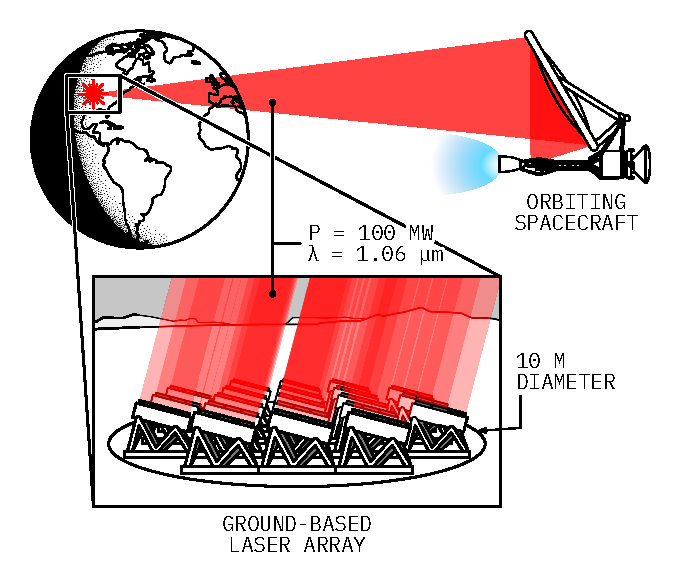
\includegraphics[width=0.4\textwidth]{assets/2 background/ltp_architecture.pdf}
            \caption{LTP architecture (\textcite{duplayArgonLaserPlasmaThruster2024a})}
            \label{fig:LTP architecture}
        \end{figure}

        In the thrust chamber of the vehicle, hydrogen is introduced. The laser is focused inside the chamber and is absorbed by the gas via inverse Bremsstrahlung, creating a Laser-Supported Plasma (LSP) core. Colder hydrogen flows around the LSP core and is heated by it to \qty{10000}{K}. The hot gas is then exhausted though a conventional converging-diverging nozzle at the exhaust velocity, imparting thrust to the vehicle.

        \begin{figure}[!ht]
            \centering
            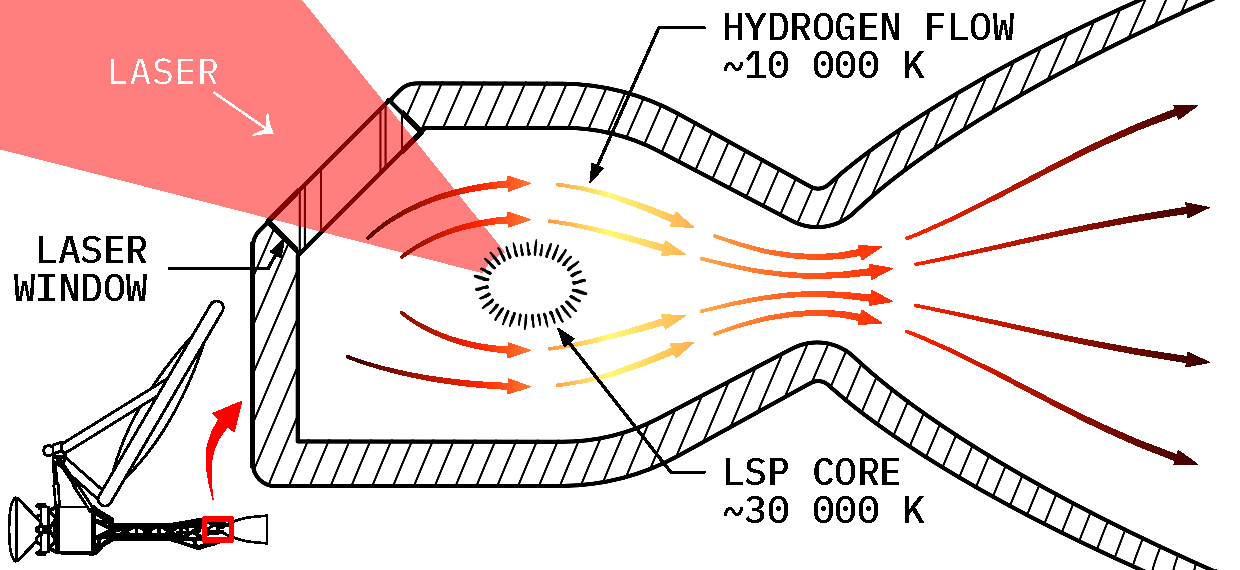
\includegraphics[width=0.6\textwidth]{assets/2 background/chamber.pdf}
            \caption{Overview of LTP system (\textcite{duplayArgonLaserPlasmaThruster2024a})}
            \label{fig:LTP system overview}
        \end{figure}

        In a conventional chemical rocket engine, the energy source is the oxidizer and the fuel, which are reacted together to release energy. They are transported with the rocket and set the temperature of the combustion reaction (typically \qtyrange{2000}{3000}{K}), which is directly related to the exhaust velocity.
        
        Separating the power source used for propulsion (here, the laser) from the spacecraft itself allows crucial weight savings, either increasing the payload mass fraction or decreasing transit time. Using a laser also allows for much greater thrust chamber temperatures than chemical propulsion, as the temperature of these plasmas is typically \qtyrange{15000}{30000}{K}. This gives in turn greater exhaust velocities. This propulsion method could therefore be an order of magnitude more efficient than our current rocket engines if certain engineering problems can be solved.

        Increasing the amount of energy deposited by the laser into the working gas remains a topic of active research and is a significant hurdle for the operational use of LTP. The two main conversion efficiencies are:
        \begin{enumerate}
            \item Absorption of the laser energy by the plasma
            \item Heat transfer from the plasma to the working gas (e.g. propellant)
        \end{enumerate}
        A selection of past LSP experiments will now be presented, with an emphasis on these efficiencies. As the efficiencies chosen are different from source to source, these will be defined where applicable.
    
    \section{Literature review}

        %Russian work: 1960s-2000s?

        The experimental basis of LTP was developed by \textcite{generalovContinuousOpticalDischarge1970} in 1970. For the first time, an LSP was generated with a \qty{150}{W} \ce{CO2} laser operating at \qty{10.6}{μm} wavelength. In this case, the LSP was initiated by a second, \qty{10}{kW} pulsed \ce{CO2} laser.
        
        %American work: 1970s-1990s?

        Work was done in the mid-1970s by \textcite{shojiLaserheatedRocketThruster1977,shojiPerformanceHeatTransfer1976a} to design a small-scale \qty{10}{kW} and full-scale \qty{5000}{kW} LTP engine. Carbon-seeded hydrogen was chosen to capture the plasma's radiation, which was mostly in the UV wavelength. \qty{20}{\%} of the laser power would be lost by convection and radiation to the walls in the \qty{10}{kW} thruster, with an additional \qty{5}{\%} of laser power lost by radiation through the thruster window. However, this was not tested. The \qty{10}{kW} prototype (\autoref{fig:Shoji apparatus}) was built and delivered to NASA at the conclusion of their effort.
        \begin{figure}[!ht]
            \centering
            \begin{subfigure}[t]{0.45\textwidth}
                \centering
                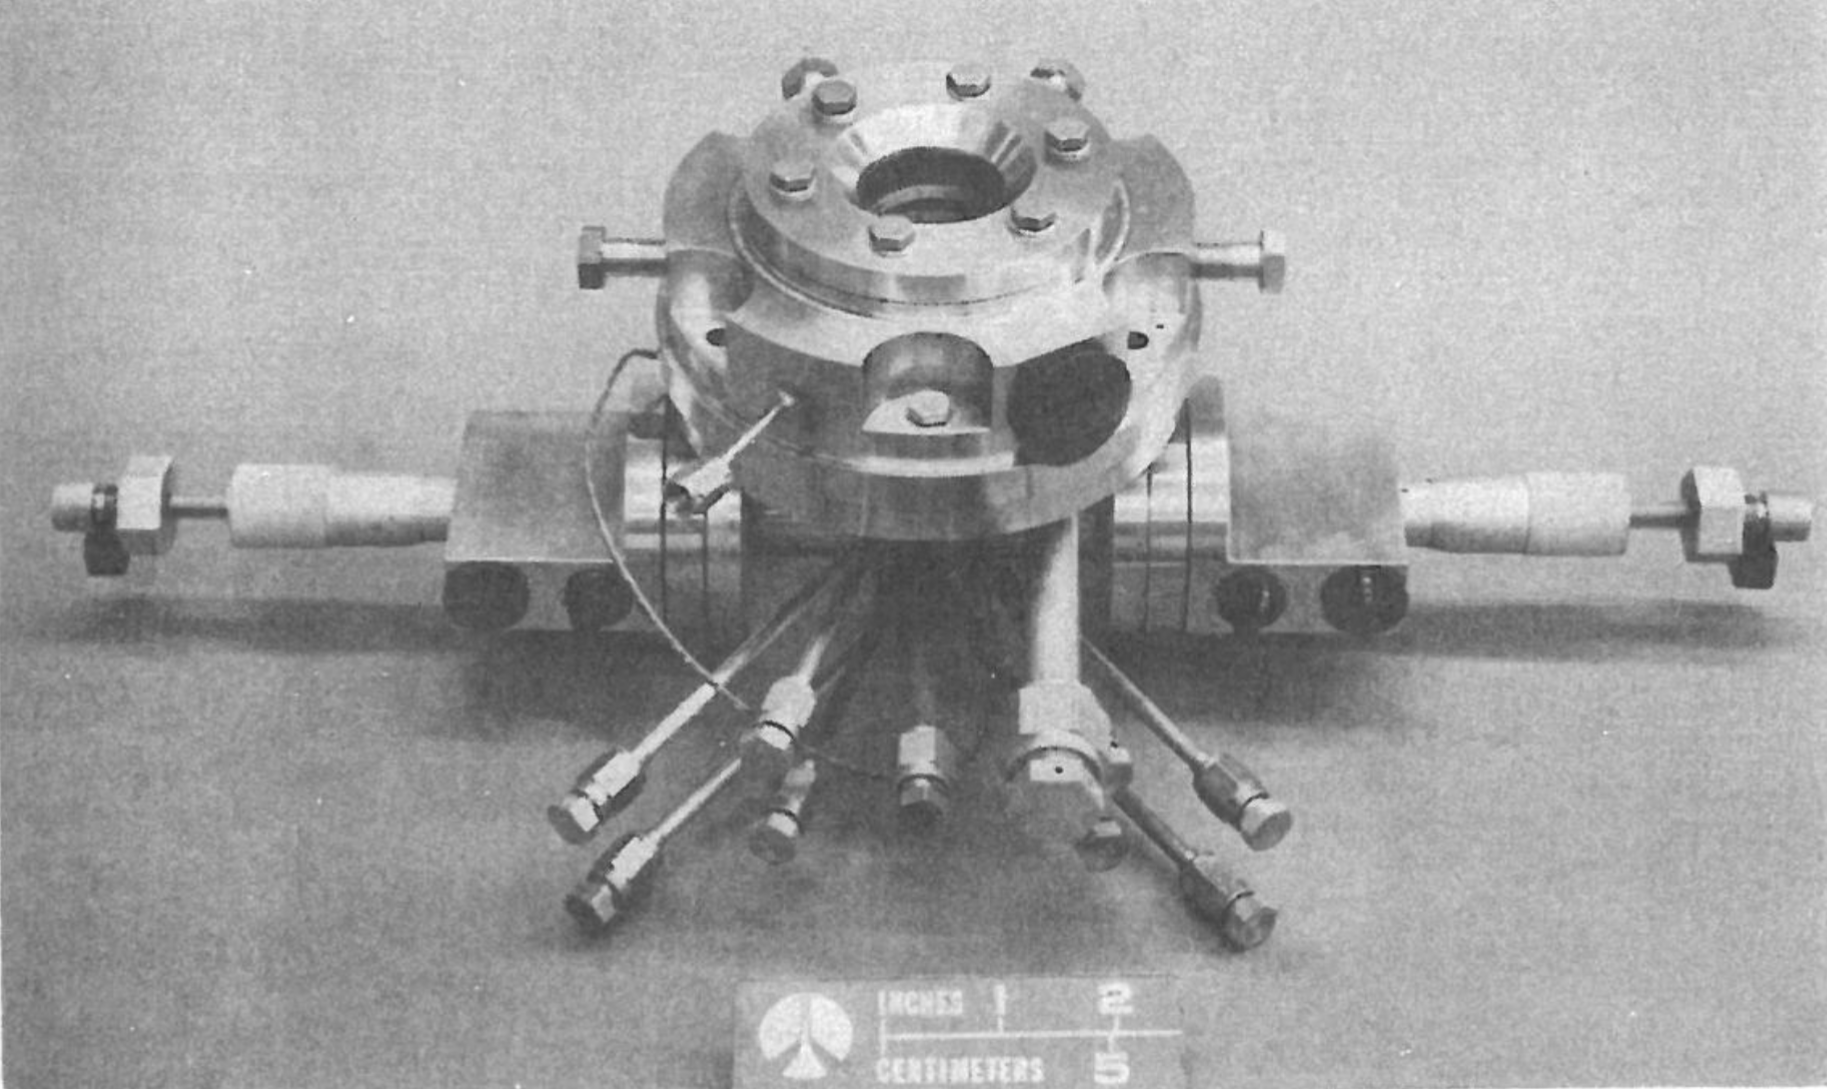
\includegraphics[width=\textwidth]{assets/2 background/Shoji_assy.png}
                \caption{\qty{10}{kW} thruster from \textcite{shojiPerformanceHeatTransfer1976a}}
                \label{fig:Shoji apparatus}
                \end{subfigure}
            \hfill
            \begin{subfigure}[t]{0.45\textwidth}
                \centering
                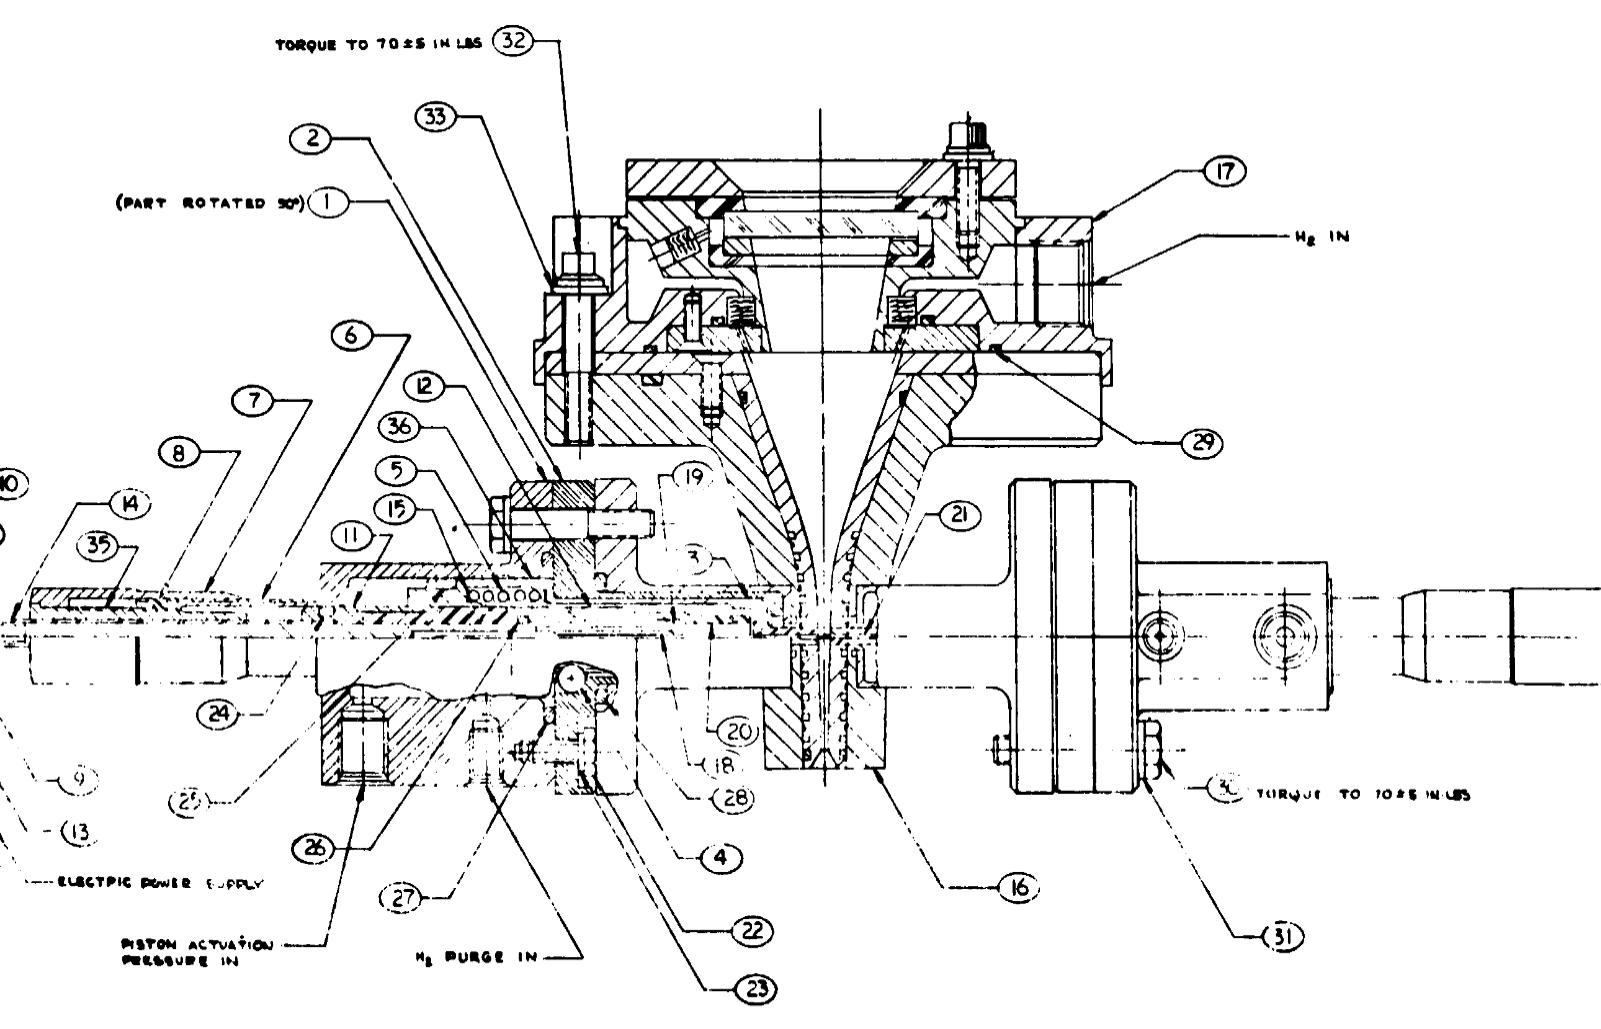
\includegraphics[width=\textwidth]{assets/2 background/Shoji cross-section.png}
                \caption{Cross-section drawing of \qty{10}{kW} thruster from \textcite{shojiLaserheatedRocketThruster1977} (original is of poor quality)}
                \label{fig:Shoji cross-section}
            \end{subfigure}
            \caption{Thruster designed by \textcite{shojiLaserheatedRocketThruster1977}}
            \label{fig:Shoji apparatussies}
        \end{figure}

        In the 1980s, \textcite{keeferPowerAbsorptionLasersustained1986a} studied LSP in a forced convective flow environment. Using a \qty{1.5}{kW} \ce{CO2} laser with power levels of \qtyrange{360}{840}{W} and pressures of \qtyrange{1.3}{2.3}{atm}, with varying argon flow velocities, the temperature field of the plasma was measured. From the temperature field, and assuming local thermodynamic equilibrium, the power absorbed by the plasma and the power radiated from it can be calculated.
        \begin{figure}[!ht]
            \centering
            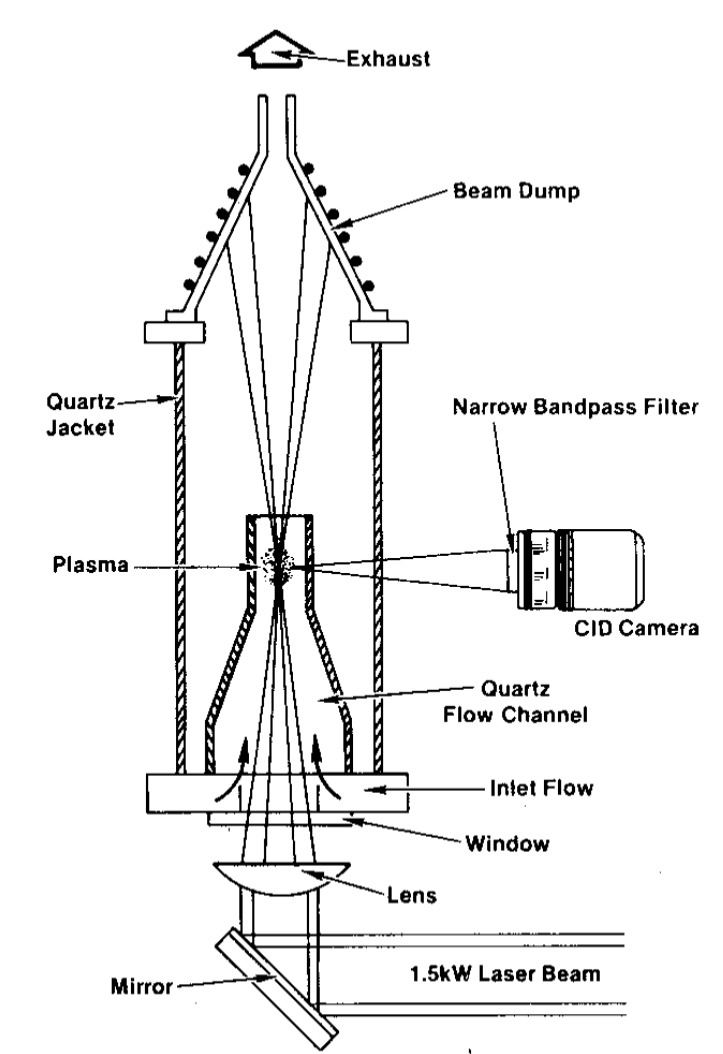
\includegraphics[width=0.4\textwidth]{assets/2 background/UTSI (Keefer) Apparatus.png}
            \caption{Experimental apparatus from \textcite{keeferPowerAbsorptionLasersustained1986a}}
            \label{fig:Keefer apparatus}
        \end{figure}
        \autoref{fig:Keefer apparatus} shows the apparatus used for these measurements. An inner quartz flow channel contained the plasma, while an outer quartz jacket contained the pressure. The plasma was initiated by laser heating of a tungsten rod, which was removed after initiation. Downstream, a water-cooled copper beam dump absorbed the energy of the laser and the heated argon flow, but was not used for measurements. The plasma's temperature was obtained through analyzing digital images. This temperature field was then used to calculate the power absorption and the radiation loss. The power absorbed by the plasma was between \qtyrange{23}{61}{\%} of incident laser power, while radiation loss was between \qtyrange{51}{80}{\%} of the absorbed power.

        Contemporary to \textcite{keeferPowerAbsorptionLasersustained1986a}, Mazumder and Krier headed a group at the University of Illinois that advanced the field of LTP. \textcite{krierContinuousWaveLaser1986a} reported laser absorption in an argon plasma approaching \qty{80}{\%}. \autoref{fig:Krier apparatus} shows the apparatus that was used by \textcite{krierContinuousWaveLaser1986a}, \textcite{zerkleLasersustainedArgonPlasmas1990} and \textcite{chenEmissionSpectroscopyCw1989a}. This vertical cylindrical flow chamber was made of 304 steel and had an internal diameter of 5 inches. A water-cooled calorimeter was used as a beam dump for the \qty{10}{kW} \ce{CO_2} laser. The laser energy not collected by the beam dump was assumed to be absorbed by the plasma, as the radiation reflected off the plasma is less than \qty{2}{\%} at these electron number densities. Moveable thermocouples gave two-dimensional maps of the flow surrounding the plasma core. The direct laser heating of the thermocouples and their carriage was taken into account.
        \begin{figure}[!ht]
            \centering
            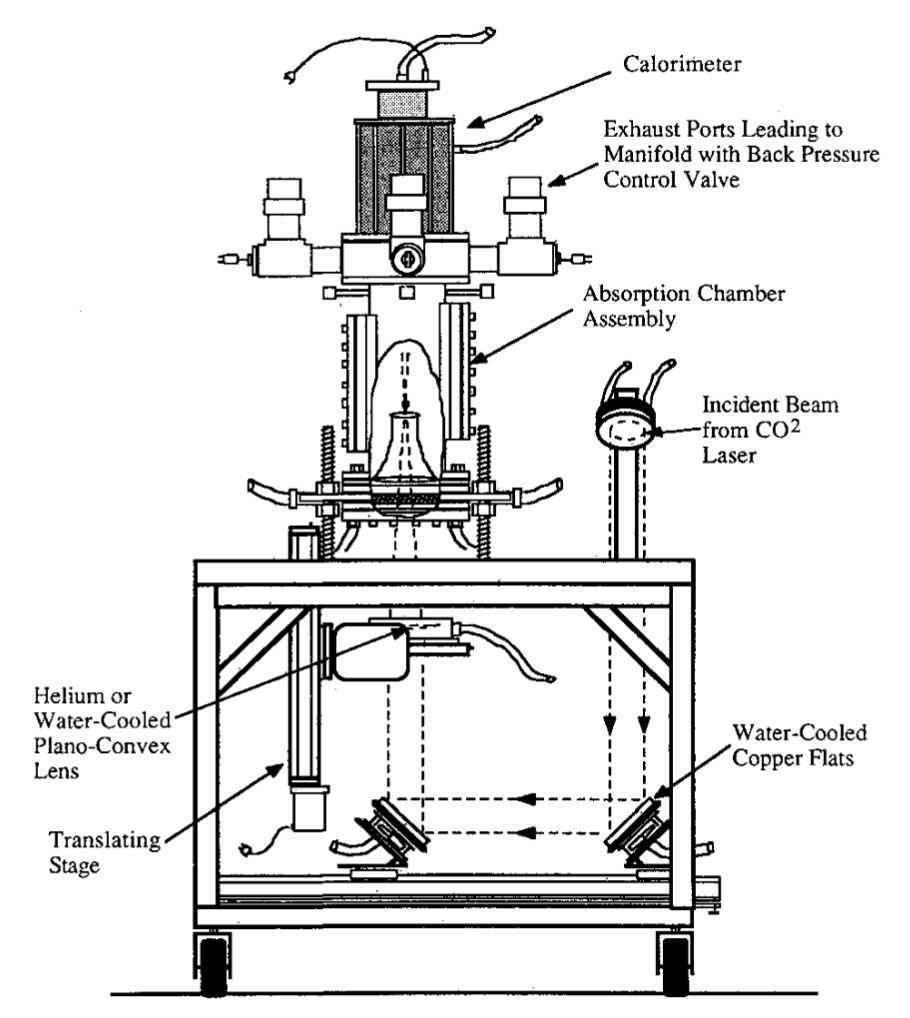
\includegraphics[width=0.5\textwidth]{assets/2 background/Illinois (Krier) Apparatus.png}
            \caption{Experimental apparatus from \textcite{zerkleLasersustainedArgonPlasmas1990}}
            \label{fig:Krier apparatus}
        \end{figure}
        These two-dimensional temperature maps \todo{INSERT EXPLANATION HERE}. Thermal efficiency was between \qtyrange{6}{25}{\%}, with radiative losses of \qty{64}{\%} and \qty{30}{\%}, 
        respectively. Thermal efficiency was defined as:


        \[\eta_\mathrm{th} =  \frac{\text{Power retained by the gas}}{\text{Incident laser power}}\]
        The minimum maintenance intensity of the plasma was also estimated at \qtyrange{0.1}{0.3}{MW/cm^2}.

        Further work by \textcite{zerkleLasersustainedArgonPlasmas1990} with the apparatus shown in \autoref{fig:Krier apparatus} reported absorption from \qtyrange{55}{97}{\%} and thermal efficiency from \qtyrange{11}{46}{\%}. This was done in \qtylist{1 2.5}{atm} of flowing argon, with laser powers up to \qty{7}{kW}. \textcite{chenEmissionSpectroscopyCw1989a} again increased the thermal efficiency of this apparatus, with \qtyrange{41}{62}{\%} of the laser energy being retained by the gas as thermal energy. This was among the highest thermal efficiencies measured by an LSP experiment. Here, \qty{86}{\%} of the laser's energy is absorbed by the LSP. This was attained with a \qty{5}{kW} \ce{CO2} laser, with flow speeds between \qtyrange{2}{10}{m/s}. They discuss that greater thermal efficiency is due to greater laser power, a high enough flow speed and a greater laser focusing $f$ number.

        Based on work by the Illinois group, an LTP engine demonstrator was tested in 1995 by \textcite{blackLaserPropulsion10kW1995} with a \qty{10}{kW} \ce{CO2} laser. This was planned to be a step towards a full-scale thruster. More than 100 thruster firings were completed, lasting 1 to 2 minutes each. The \qty{10}{kW} thruster is presented in \autoref{fig:Black apparatus}. It is mounted in a vacuum chamber to a thrust measurement assembly. Efficiency was calculated from:
        \[ \eta = \frac{F^2}{2 \dot{m} P_\mathrm{L}} \]
        with $P_\mathrm{L}$ the input laser power at the thruster window. Both argon and hydrogen were used. Argon propellant produced \qty{200}{s} of $I_\mathrm{sp}$ and a peak efficiency of 0.24. With hydrogen propellant, an $I_\mathrm{sp}$ of \qty{350}{s} and a peak efficiency of 0.37 were reported.
        \begin{figure}[!ht]
            \centering
            \begin{subfigure}[t]{0.3\textwidth}
                \centering
                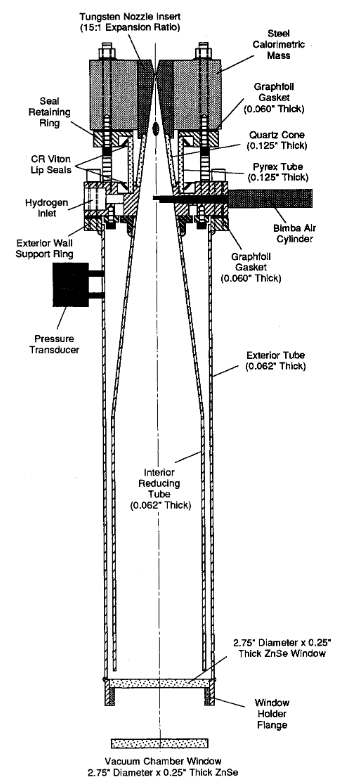
\includegraphics[width=\textwidth]{assets/2 background/BlackKrier thruster.png}
                \caption{\qty{10}{kW} thruster}
                \label{fig:Black apparatus}
            \end{subfigure}
            \hfill
            \begin{subfigure}[t]{0.45\textwidth}
                \centering
                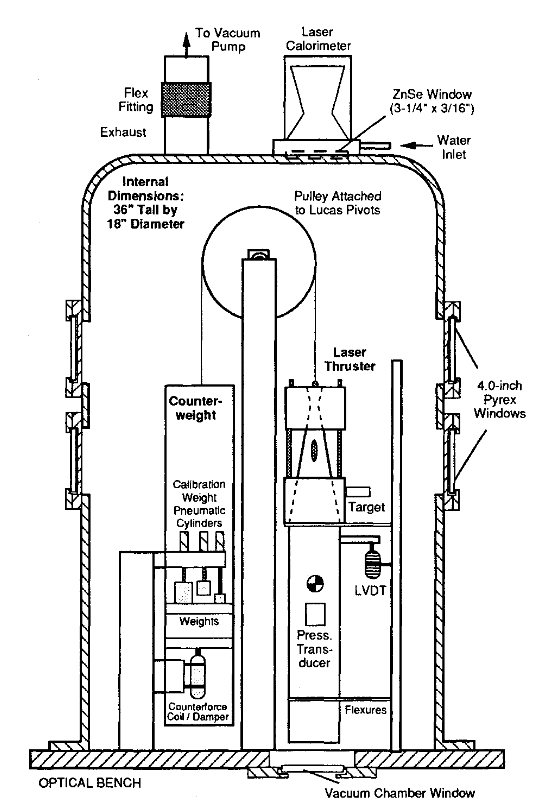
\includegraphics[width=\textwidth]{assets/2 background/Black thrust measurement assy.png}
                \caption{Thrust measurement assembly}
                \label{fig:Black thrust measurement}
            \end{subfigure}
            \caption{Apparatus used in \textcite{blackLaserPropulsion10kW1995}}
            \label{fig:Black apparatussies}
        \end{figure}
        A preliminary design for the full-scale \qty{100}{kW} thruster was also presented, with a predicted specific impulse of \qty{1000}{s}, thrust of \qty{4.5}{N} and a conversion efficiency of \qty{80}{\%}.

        %Chinese and Japanese work: 1980s-2020s

        In the early 2000s, \textcite{toyodaThrustPerformanceCW2002} built and tested two different thruster models, presented in \autoref{fig:Toyoda apparatussies}. These thrusters, using argon or nitrogen heated by LSP, were powered by a \qty{2}{kW} \ce{CO2} laser. The LSPs were initiated by a retractable tungsten rod at the laser's focus. Thrust measurements were done both in atmospheric pressure and in vacuum. This comparative study showed that confining the plasma into a smaller chamber increased heat transfer and therefore, efficiency. \textcite{toyodaThrustPerformanceCW2002} defined the energy conversion efficiency as the amount of laser power that is converted into usable kinetic energy for thrust. It is calculated as\footnote{As mentioned by \textcite{duplayArgonLaserPlasmaThruster2024a}, there appears to be a typographical error in the reference as the units are inconsistent. The corrected equation is presented here.}:
        \[ \eta_\mathrm{e} =  \frac{F^2_\mathrm{hot} -F^2_\mathrm{cold}}{2 \dot{m} P}\]
        Where $F_\mathrm{hot}$ is the thrust with laser on, $F_\mathrm{cold}$ is the cold flow thrust (laser off) and $P$ is incident laser power. An energy conversion efficiency of 37\% and an $I_\mathrm{sp}$ of \qty{113}{s} were measured with the second model \autoref{fig:Toyoda apparatus 2} in vacuum with argon propellant. The pressure ratio, defined as the chamber pressure divided by the nozzle exit pressure, was 420. A water cooling system measured the heat loss to the walls to be 55\% of incident laser power, with a final 8\% being ``other loss". Heat loss to the walls was expected to be recycled with regenerative cooling in a real-world application.

        \begin{figure}[!ht]
            \centering
            \begin{subfigure}[t]{0.45\textwidth}
                \centering
                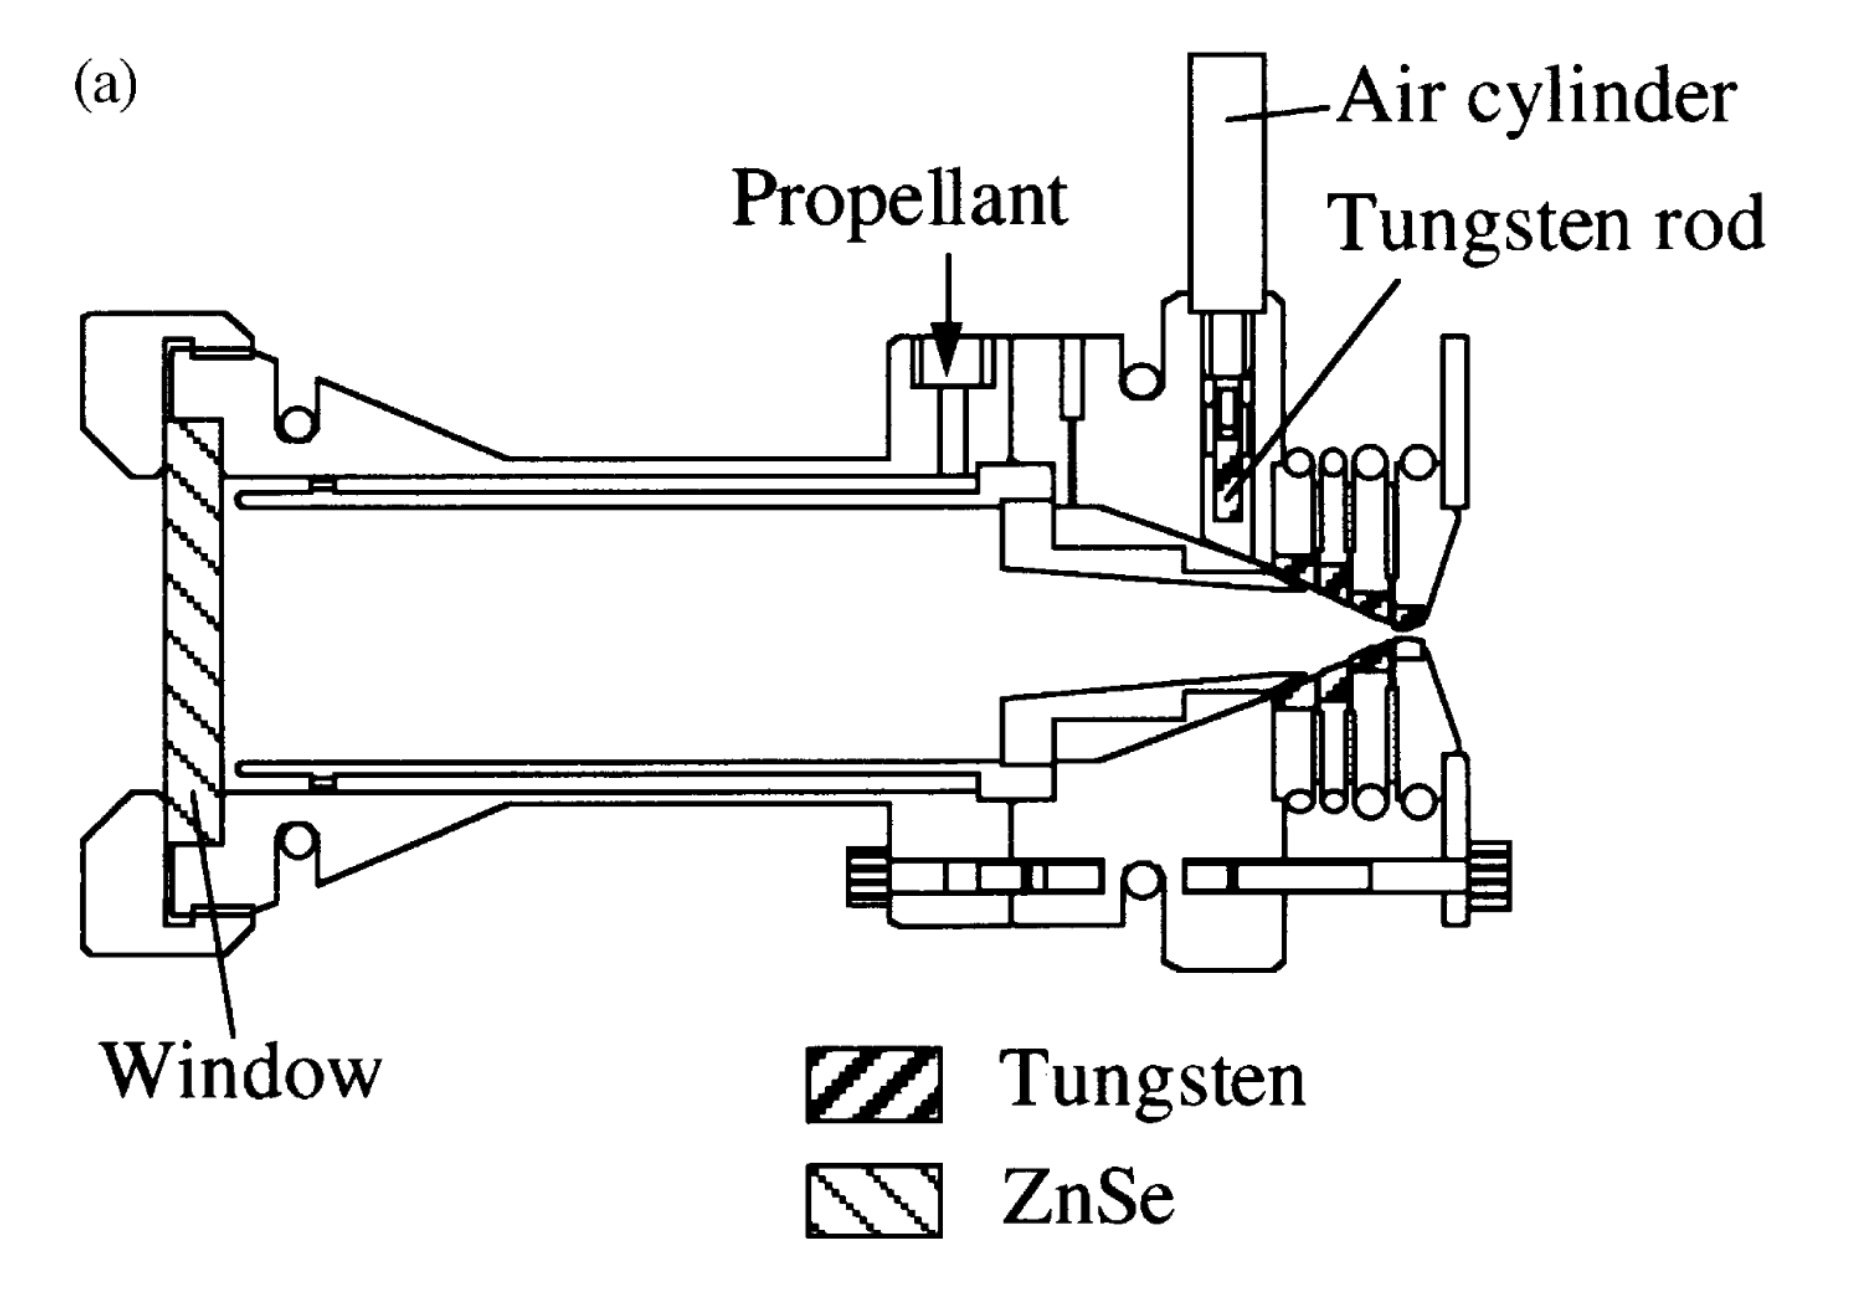
\includegraphics[width=\textwidth]{assets/2 background/Toyoda apparatus model 1.jpg}
                \caption{Model I}
                \label{fig:Toyoda apparatus 1}
            \end{subfigure}
            \hfill
            \begin{subfigure}[t]{0.45\textwidth}
                \centering
                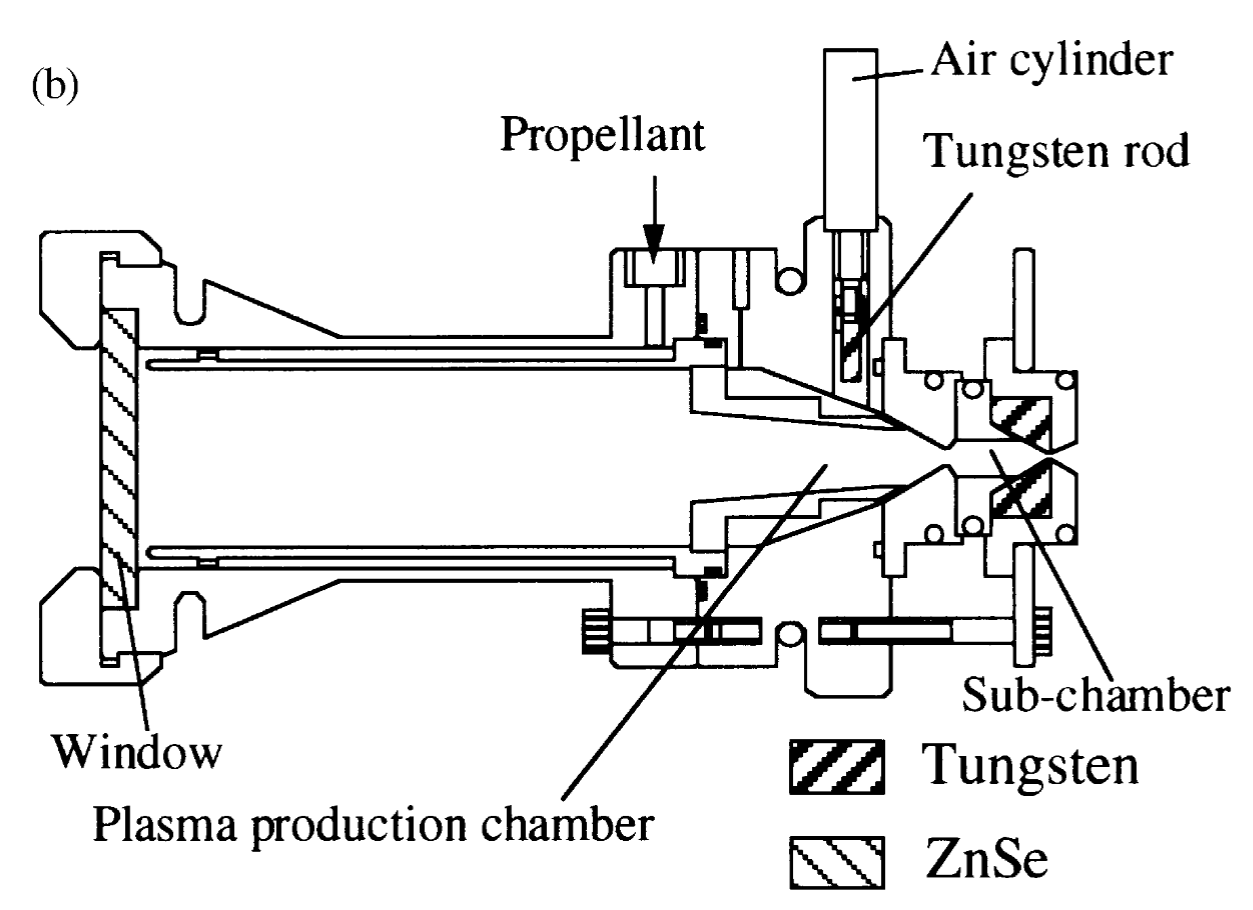
\includegraphics[width=\textwidth]{assets/2 background/Toyoda Apparatus model 2.png}
                \caption{Model II}
                \label{fig:Toyoda apparatus 2}
            \end{subfigure}
            \caption{Two thruster models from \textcite{toyodaThrustPerformanceCW2002}}
            \label{fig:Toyoda apparatussies}
        \end{figure}

        \textcite{luCharacteristicDiagnosticsLaserStabilized2022a} investigated LSP for lighting applications instead of propulsion. Therefore, an emphasis was made on spectroscopy measurements. A \qty{300}{W} fiber laser at a wavelength of \qty{1080}{nm} was focused to a \qty{50}{μm} diameter spot in a high pressure chamber.
        \begin{figure}[!ht]
            \centering
            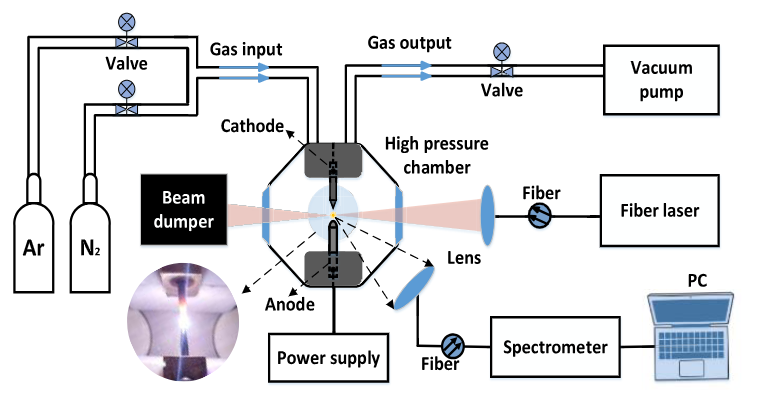
\includegraphics[width=0.7\textwidth]{assets/2 background/Lu apparatus.png}
            \caption{Experimental setup from \textcite{luCharacteristicDiagnosticsLaserStabilized2022a}}
            \label{fig:Lu apparatus}
        \end{figure}
        Argon was used, with pressures between \qtyrange{10}{20}{bar}. A lower initiation power (\qty{117}{W}) than other studies was achieved at \qty{20}{bar}. This was attributed to the smaller focus delivering a greater photon flux. \ce{N2} was later added between \qtyrange{0.1}{1.0}{\%}. As expected, increasing the laser power or the gas pressure was found to increase the radiation intensity of the LSP. However, adding \ce{N2} reduced both the electron temperature and electron density of the LSP, reducing its radiation intensity.

        Seeding the working gas with another species has been discussed as a way to increase the energy absorption into the working fluid of an LTP engine. LSPs in pure methane and methane-seeded gasses have been investigated by \textcite{kameiMethaneMethaneXenon2020}. Methane dissociates into hydrogen and carbon with the high temperature of the LSP. As mentioned with \textcite{shojiLaserheatedRocketThruster1977}, carbon particles would absorb the LSP's UV radiation.  A \qty{1.1}{kW} diode laser at a wavelength of \qty{940}{nm} was beamed into a high-pressure chamber fitted with arc initiation electrodes. The gap between these electrodes was \qty{1}{mm}. A CCD type spectrometer recorded emission spectra of the initiation arc discharge and of the LSP. LSPs in three different gasses were attempted: pure methane, methane-argon, and methane-xenon.
        
        In methane at \qty{0.1}{MPa}, soot formation between the electrodes prevented LSP initiation. The spectrometer confirmed the dissociation of methane, as line spectra of carbon and hydrogen were observed at the initiation arc. Initiation was also unsuccessful in argon-methane with a pressure between \qtyrange{0.1}{0.3}{MPa} and a methane volume fraction between \qtyrange{20}{60}{\%}. LSP was successfully generated in methane-xenon, with a lower threshold power (\qty{850}{W}) than in pure xenon. The partial pressure of methane was between \qtyrange{0.02}{0.6}{MPa}, with a partial pressure of xenon of \qty{0.10}{MPa}.

        \textcite{takanoDemonstrationDiodeLasersustained} used a diode laser emitting simultaneously at \qty{927}{nm} and \qty{951}{nm} to generate LSPs in argon. This resulted in an $I_\mathrm{sp}$ of \qty{105}{s} and a thrust efficiency of \qty{8}{\%}. This $I_\mathrm{sp}$ was calculated from the plenum pressure when the laser was on. They define thrust efficiency as:
        \[
        \eta = \frac{g_0 I_\mathrm{sp} (F_\mathrm{hot}-F_\mathrm{cold})}{2 P_\mathrm{laser}}
        \]
        Two setups were used: the LSP generation chamber previously used by \textcite{kameiMethaneMethaneXenon2020} (\autoref{fig:Takano LSP generation chamber}) and an LSP thruster (\autoref{fig:Takano LSP thruster}).
        \begin{figure}[!ht]
            \centering
            \begin{subfigure}[t]{0.45\textwidth}
                \centering
                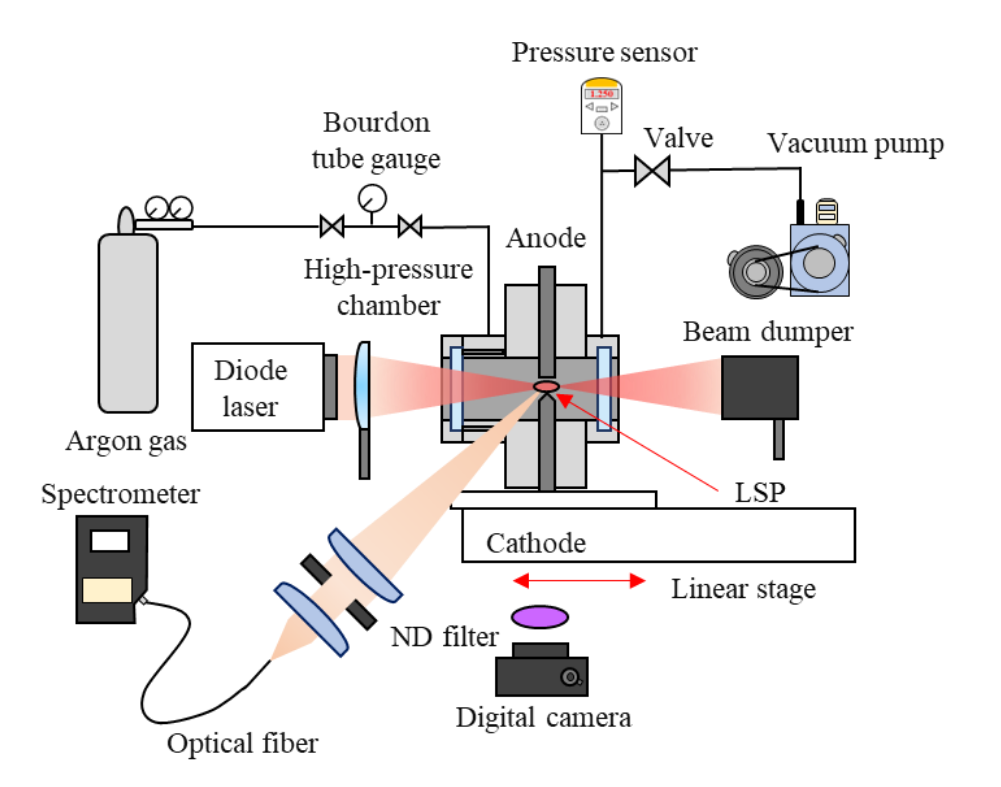
\includegraphics[width=\textwidth]{assets/2 background/Takano LSP chamber.png}
                \caption{LSP generation chamber and systems}
                \label{fig:Takano LSP generation chamber}
            \end{subfigure}
            \hfill
            \begin{subfigure}[t]{0.45\textwidth}
                \centering
                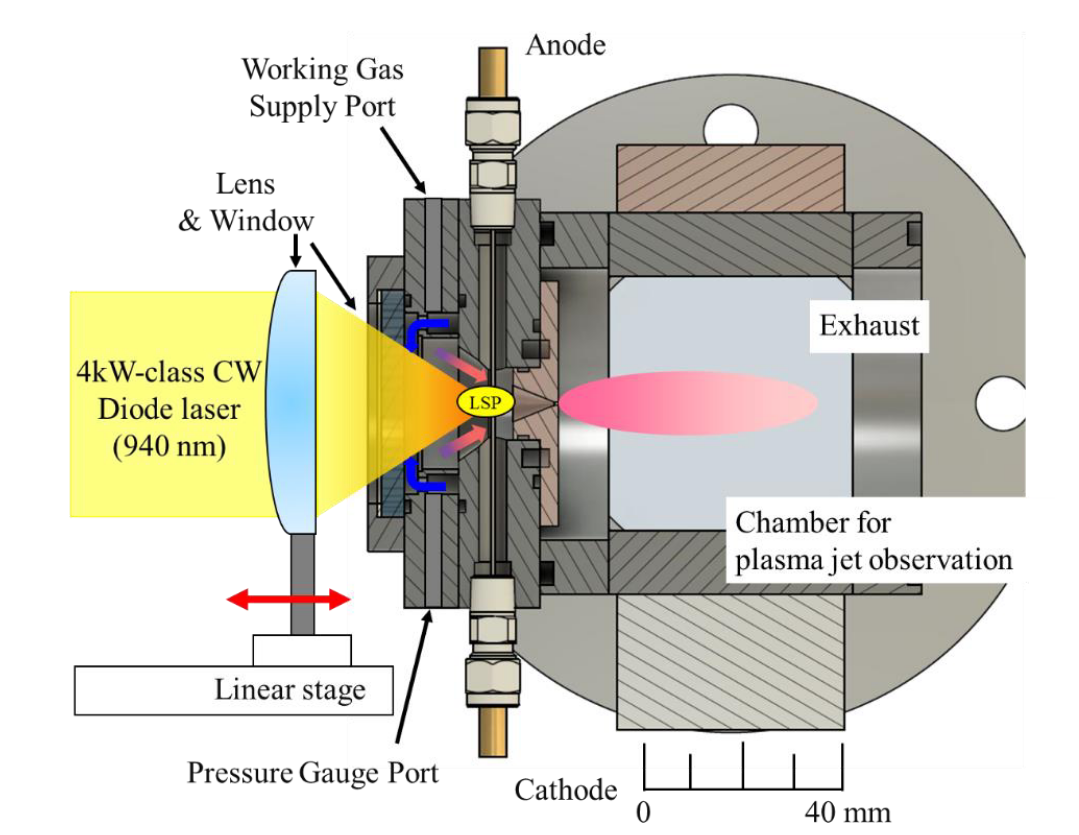
\includegraphics[width=\textwidth]{assets/2 background/Takano LSP thruster.png}
                \caption{LSP thruster}
                \label{fig:Takano LSP thruster}
            \end{subfigure}
            \caption{LSP setups from \textcite{takanoDemonstrationDiodeLasersustained}}
            \label{fig:Takano apparatussies}
        \end{figure}
        The LSP chamber was used to determine the effect of various F-numbers on the argon LSP. The thruster has an interchangeable copper throat, with diameters of \qty{0.7}{mm} and \qty{1.0}{mm}. In both setups, electric arc initiation was used. Once initiated in the thruster, the LSP is moved toward the nozzle with the lens mounted on a motorized stage. It was found that moving the LSP this way increased the heat exchange with the working gas. Thrust was calculated by using the pressure measurements inside the thruster's heating chamber.

        %Canadian work: 2020s  

        \textcite{duplayArgonLaserPlasmaThruster2024a} used a \qty{3}{kW} pulsed fiber laser to create LSPs in static and flowing argon. In static argon, about \qty{80}{\%} of the laser energy was being absorbed by the plasma, with approximately \qty{15}{\%} of the laser energy heating the bulk gas. This was done between \qtyrange{5}{20}{bar}.
        \begin{figure}[!ht]
            \centering
            \includegraphics[width=0.7\textwidth]{assets/2 background/finalsetup_static.pdf}
            \caption{Static LSP apparatus from \textcite{duplayArgonLaserPlasmaThruster2024a}}
            \label{fig:Duplay apparatus}
        \end{figure}

    \section{Summary and direction of work in this thesis}
        
        From the literature review, \autoref{tab:lit review summary} and \autoref{tab:efficiencies} were compiled. Most studies have used \ce{CO2} lasers with a wavelength of \qty{10.6}{μm}. Use of a \ce{CO2} laser for power beaming to a remote target for propulsion applications is limited by the range over which the laser can be focused due to their long laser wavelength. 
    
        Indeed, the diffraction limit of a laser, which is the theoretical lower limit on beam divergence, equals the wavelength ($\lambda$) divided by the diameter $D$ of the output beam \cite{hechtUnderstandingLasersEntry2019}.
        \[
        \text{Diffraction limit (radians)} = \lambda/D
        \]
        This relegated \ce{CO2} lasers to ground-to-orbit launch. Recently, high power fiber lasers emitting near \qty{1}{μm} have become readily available. Being able to beam energy to low earth orbit, fiber lasers make laser propulsion more feasible.

        \begin{table}[!ht]
            \centering
            \caption{Summary of a selection of past LSP experiments. $\lambda$: wavelength, $P$: maximum laser power, $p$: pressure, $\dot m$: mass flow rate, $I_\mathrm{sp}$: maximum specific impulse, $F_\mathrm{T}$: maximum thrust}
            \label{tab:lit review summary}
            \begin{tabularx}{\textwidth}{@{}>{\small}X<{\raggedright}lXXrXXXrr<{\raggedright}@{}}
            \toprule
            {\normalsize LSP   Facility} & Year & Laser & $\lambda$ [\unit{\um}] & $P$ [kW] & Gas & $p$ [atm] & $\dot m$ [g/s] & $I_\mathrm{sp}$ [s] & $F_\mathrm{T}$ [N]  \\ \midrule
            \textcite{generalovContinuousOpticalDischarge1970}        &1970&\ce{CO_2}&10.60&0.15 &\ce{Xe}           & 3.0-4.0  &  -  & -   &  -   \\
            \textcite{keeferPowerAbsorptionLasersustained1986a}       &1986&\ce{CO_2}&10.60&0.84 &\ce{Ar}           & 1.3-2.3  & 0.01-0.19   & -   &  -   \\
            \textcite{krierContinuousWaveLaser1986a}                  &1986&\ce{CO_2}&10.60&10  &\ce{Ar}           &     -       & 2.3-4.6 & -& -\\
            \textcite{zerkleLasersustainedArgonPlasmas1990}           &1988&\ce{CO_2}&10.60&7   &\ce{Ar}           &      -      &     -     & -&- \\
            \textcite{chenEmissionSpectroscopyCw1989a}                &1989&\ce{CO_2}&10.60&5   &\ce{Ar}           &      -      &  -  & -   & -    \\
            \textcite{blackLaserPropulsion10kW1995}                   &1995&\ce{CO_2}&10.60&10  &\ce{Ar}           & 1.4-2.4  & 5.1-9.4 & 200 & 7 \\
                                                                      &    &\ce{CO_2}&10.60&10  &\ce{H_2}          &    3.4        & 1.1&  350   & 3 \\
            \textcite{toyodaThrustPerformanceCW2002}                  &2002&\ce{CO_2}&10.60&2   &\ce{Ar}, \ce{N_2} & 2.0-5.5  &  -  & 113 & 0.44 \\
            \textcite{luCharacteristicDiagnosticsLaserStabilized2022a}&2022&Fiber    &1.08 &0.30 &\ce{Ar}, \ce{N_2} & 9.9-19.7 &  -  & -   & -    \\ 
            \textcite{takanoDemonstrationDiodeLasersustained}         &2024&Diode    &0.927 and 0.951 &4.4 &\ce{Ar}   & 10-15 &   - & 105   & -    \\
            \textcite{duplayArgonLaserPlasmaThruster2024a}            &2024&Fiber    &1.07  & 3 &\ce{Ar}            &   5-20  & 0 & - & - \\
            \bottomrule
            \end{tabularx}
        \end{table}

        \begin{table}[!ht]
            \centering
            \caption{Comparative table of experimental LTP thruster efficiencies}
            \label{tab:efficiencies}
            \begin{tabularx}{\textwidth}{@{}>{\small}X<{\raggedright} r l r@{}}
            \toprule
            {\normalsize LSP   Facility}   & Laser absorption  & Efficiency & Value of efficiency \\ \midrule
            \textcite{keeferPowerAbsorptionLasersustained1986a}   & 0.23 - 0.61      &          -        &                 -          \\
            \textcite{krierContinuousWaveLaser1986a}       & 0.50 - 0.80         & $\eta_\mathrm{th} =  \frac{\text{Power retained by the gas}}{\text{Incident laser power}}$ &  0.06 - 0.25 \\
            \textcite{zerkleLasersustainedArgonPlasmas1990}       & 0.55 - 0.97   &         $\eta_\mathrm{th} =  \frac{\text{Power retained by the gas}}{\text{Incident laser power}}$ &  0.11 - 0.46 \\
            \textcite{chenEmissionSpectroscopyCw1989a}          & 0.86                      &  $\eta_\mathrm{th} =  \frac{\text{Power retained by the gas}}{\text{Incident laser power}}$  &  0.41-0.62  \\
            \textcite{blackLaserPropulsion10kW1995}       &  -  & $ \eta = \frac{F_\mathrm{hot}^2}{2 \dot{m} P_\mathrm{L}} $& 0.20 - 0.25 (Ar), 0.25 - 0.40 (H)     \\
            \textcite{toyodaThrustPerformanceCW2002}    & -                      & $ \eta_\mathrm{e} =  \frac{F^2_\mathrm{hot} -F^2_\mathrm{cold}}{2 \dot{m} P} $     &   0.37 \\
            \textcite{takanoDemonstrationDiodeLasersustained}  &       -       & $ \eta = \frac{g_0 I_\mathrm{sp} (F_\mathrm{hot}-F_\mathrm{cold})}{2 P_\mathrm{laser}} $ & 0.08 \\ 
            \textcite{duplayArgonLaserPlasmaThruster2024a}  &  0.80&  $\eta_\mathrm{th} =  \frac{\text{Power retained by the gas}}{\text{Incident laser power}}$ & 0.15 \\
            \bottomrule
            \end{tabularx}
        \end{table}
        

        To increase thermal efficiency, \textcite{chenEmissionSpectroscopyCw1989a} suggest:
        \begin{enumerate}
            \item A greater laser power, which gives greater inverse bremsstrahlung absorption coefficient and longer absorption path length;
            \item A high enough flow speed to push the LSP back to the laser focus, but not too fast as to blow the plasma out;
            \item A greater laser focusing $f$ number, creating a longer and narrower plasma. This increases the probability a photon will be absorbed by the plasma and reduces the radiation loss.
        \end{enumerate}

        For a small-scale demonstration thruster, $I_\mathrm{sp}$ values near \qty{100}{s} can be expected, with thrust values under \qty{1}{N}, as was found by \textcite{toyodaThrustPerformanceCW2002} and \textcite{takanoDemonstrationDiodeLasersustained}.

        % Previous objective: The objective of this research project will be to test a lab-scale proof-of-concept LTP thruster for interplanetary space flight, using a \qty{1.07}{μm} fiber laser. Key performance parameters of this thruster such as thrust and specific impulse will be measured, and the LSP heating core inside the thruster will be characterized. 
        
        
        The objective of this research project will be to test a lab-scale proof-of-concept LTP thruster for interplanetary space flight, using a \qty{1.07}{μm} fiber laser \todo{add to this}. This project will mainly build upon the experimental research started by \textcite{duplayArgonLaserPlasmaThruster2024a}.
        
        % Link to next chapter, modelling c_p
        Before going into experiments, it is important to characterize certain thermodynamic properties of the gasses used. Notably, the modelling of heat capacity will be presented in the next chapter.

    \chapter{Background} \label{chp:background}
    \section{Russian work: 1960s-2000s?}
    \section{American work: 1970s-1990s?}
    \section{Japanese work: 1980s-2020s?}
    \section{Chinese work: 2020s?}
    \section{Canadian work: 2020s}
    \section{Summary and direction of work in this thesis}

        \begin{table}[ht]
            \small
            \centering
            \caption{Summary of a selection of past LSP experiments. $\lambda$: wavelength, $P$: maximum laser power, $p$: pressure, $I_\mathrm{sp}$: maximum specific impulse, $F_\mathrm{T}$: maximum thrust}
            \label{tab:pastexp}
            \begin{tabularx}{\textwidth}{@{}>{\small}X<{\raggedright}llrrlrrr>{\footnotesize}X<{\raggedright}@{}}
            \toprule
            {LSP   Facility}                                                           & Year & Laser         & $\lambda$   [\unit{\um}] & $P$ [kW] & Gas                 & $p$   [atm] & $I_\mathrm{sp}$ [s] & $F_\mathrm{T}$   [N] & {Comments}                                                                   \\ \midrule
            \textcite{generalovContinuousOpticalDischarge1970}                                                         & 1970 & \ce{CO_2}                  & 10.60             & 0.15               & \ce{Xe}              & 3.0 - 4.0        &           -             &       -       & First   LSP                                                                \\
            \textcite{keeferPowerAbsorptionLasersustained1986}         & 1986 & \ce{CO_2}                  & 10.60             & 0.84        & \ce{Ar}              & 1.3   - 2.3      &            -            &       -       & Specialized   laser beam dump integrated within the converging exit nozzle \\
            \textcite{blackLaserPropulsion10kW1995}          & 1995 & \ce{CO_2}                  & 10.60             & 10.00              & \ce{Ar},   \ce{H_2}    & 1.0   - 2.7      & 350                    & 3.00         & 15:1   expansion ratio nozzle                                              \\
            \\
            \textcite{toyodaThrustPerformanceCW2002} & 2002 & \ce{CO_2}                  & 10.60             & 2.00               & \ce{Ar},   \ce{N_2}    & 2.0   - 5.5      & 113             & 0.44         & Tungsten   rod ignition                                                    \\
            \textcite{zimakovInteractionNearIRLaser2016}                                                        & 2016 & Fiber                & 1.07              & 1.50        & \ce{Ar},   \ce{Xe}   & 3.0   - 24.7     & -                      & -            & Arc   discharge ignition                                                   \\
            \textcite{matsuiGeneratingConditionsArgon2019}                                                          & 2019 & Fiber &      1.07             &        2.00            &           \ce{Ar}           &          1.0 - 64.2        &            -            &       -       & Arc   discharge ignition                                                   \\
            \textcite{luCharacteristicDiagnosticsLaserStabilized2022a}                                                             & 2022 & Fiber                & 1.08              & 0.30      & \ce{Ar},   \ce{Ar + N_2} & 9.9   - 19.7     & -                      & -            & Arc   discharge ignition                                                   \\ \bottomrule
            \end{tabularx}
        \end{table}

        The original contribution of this work 


        % Higgins text from email to Mark Wolverton: Laser thermal propulsion originated with Arthur Kantrowitz, who was involved in developing the first gas dynamic lasers that would be able to reach MW-class power in the 1960s. (Interesting connection to Jordin Kare: Jordin was also a filk-singer, which is a science-fiction themed version of folk singing. He actually wrote a song about laser thermal propulsion called “Kantrowitz 1972”. Put your coffee cup down before listening to this…) 
        %The laser-thermal rocket kind of died with the demise of high-power laser weapon research in the early 1990s. Now with Phil Lubin’s work, I think it is worthwhile looking at again. Even with a gigawatt-class laser, laser propulsion is not well suited for ground-to-orbit launch vehicles, unless they are very small (this is what Jordin’s filk song is about—rapid turn around of launching many microlaunchers using a laser).  Here’s the clip of Elon Musk making the same point: https://youtu.be/viRylmoFAj0?si=MzzsBkhHF71FLCRG
        %However, with Philip Lubin’s demonstration that phased array lasers can be made arbitrarily large, we can now reach much deeper into space and perform propulsive maneuvers more leisurely (say, over hours), so the power requirements now drop to the 100s of MW (rather than 10s of gigawatts!). This was the basis of our 45-days-to-Mars study, which I think you have already seen. Here is an un-paywalled version of it: [2201.00244] Design of a rapid transit to Mars mission using laser-thermal propulsion (arxiv.org)
        %The other approach is to provide laser power onto a solar panel (although one tuned to the laser wavelength) that then powers electric propulsion like an ion engine or Hall effect thruster: Laser-electric propulsion. Lubin’s group published a similar study to ours, trying to hit similar objectives (the usual “Mars in a month” metrics). I’ve attached their paper here: SheerinLubinEtAl_FastTransporationElectricPropulsionDirectedEnergy_ActaAstro2021
        %Their paper and ours make for a nice “compare and contrast” of the pluses and minuses of the laser-electric and laser-thermal approaches.

    \chapter{Facility design}

    \section{Version 1 test section} \label{sec:design_v1}

        The design process of the first generation thruster, called Version 1 (V1), can be found in \textcite{duplayArgonLaserPlasmaThruster2024a}. It proved to be a dependable prototype, repurposed from a previous unrelated experiment. However, it presented problems that required a second generation prototype to be designed and manufactured.

        \begin{figure}[!ht]
            \centering
            \begin{subfigure}[t]{\textwidth}
                \includegraphics[width=0.85\textwidth]{assets/3 design/finalsetup_static.pdf}
                \caption{Static setup}
            \end{subfigure}
            \hfill
            \begin{subfigure}[t]{\textwidth}
                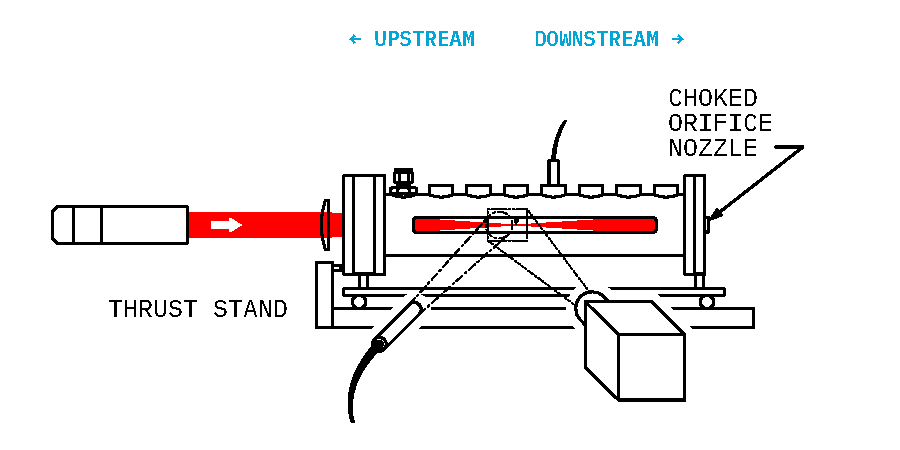
\includegraphics[width=0.85\textwidth]{assets/3 design/finalsetup_flowing.pdf}
                \caption{Flowing setup}
            \end{subfigure}
            \caption{V1 LTP thruster}
            \label{fig:V1 setup}
        \end{figure}

        298 recorded pulsed laser shots were conducted with V1, exploring the power-pressure threshold, wire initiation and spark initiation. A side window permitted direct visualization of the LSP with a high speed camera (Photron Fastcam SA5).

        % Adding holes on bottom for wire ignition

        However, this test section was made of steel, creating too much friction on its rails during thrust tests. This was mitigated in part by a rope system mentioned in \textcite{duplayArgonLaserPlasmaThruster2024a}, but was not found to be repeatable. Having the LSP heat a smaller internal volume than the \qty{0.4}{L} of V1 was also desirable, as a greater effect on internal pressure and thrust would be seen.

        Critically, rubber seals were exposed to the laser path during continuous (CW) lasing with a lower focal length lens (picture), severely burning them in the only CW test conducted. A shorter test section designed for a \qty{100}{mm} focal length lens would solve this.

    \section{Version 2} \label{sec:design_v2}

        To improve upon the V1 facility, an entire LTP thruster redesign was done. This resulted in the much smaller Version 2 (V2) purpose-built LTP thruster at the end of April 2024.

        \subsection{Requirements}

            The following requirements were developed for the design of the V2 thruster. The objective was to detect a measurable difference in thrust between an argon cold gas thruster and an argon “hot gas” thruster, heated by a laser supported plasma (LSP).

            \begin{enumerate}
                \item Laser thruster
                \begin{enumerate}
                    \item A \qty{300}{W} Continuous Wave (CW) \qty{1070}{nm} laser shall sustain the plasma (Nominal power \qty{300}{W}, actual max power \qty{350}{W})
                    \item The thruster shall have a minimum safe “hot” operation time of \qty{30}{s}
                    \begin{enumerate}
                        \item In the event of failed LSP initiation, the thruster shall safely absorb the total laser power for at least \qty{10}{s}
                    \end{enumerate}
                    \item An optical path shall be present to let the laser into the thruster, utilizing a \qty{100}{mm} focal length lens at minimum and a collimated beam with a maximum diameter of \qty{30}{mm}
                    \begin{enumerate}
                        \item The optical components shall not be damaged by the laser flux
                    \end{enumerate}
                    \item Argon shall be used as the working fluid
                    \begin{enumerate}
                        \item The argon feed gas shall be at room temperature
                    \end{enumerate}
                    \item A gas feed path shall bring argon gas into the thruster
                    \begin{enumerate}
                        \item The gas feed shall be choked at the thruster inlet
                        \item The gas feed shall be evenly distributed in the thruster
                    \end{enumerate}
                    \item The mass flow rate of the argon gas shall be measured and controlled by interchangeable upstream choked orifices
                    \item The maximum allowable operating pressure (MAOP) of the thruster shall be 50 bar
                    \begin{enumerate}
                        \item The nominal pressure of the thruster shall be 25 bar
                    \end{enumerate}
                    \item A converging-diverging exhaust nozzle shall be designed to accelerate the gas to a supersonic speed
                    \begin{enumerate}
                        \item The nozzle shall be easily changeable
                    \end{enumerate}
                    \item A 1/8" NPT port for a pressure transducer shall be present along the thruster
                    \item An optical port shall be present for spectrometry measurements of the plasma
                    \item The thruster shall be installed on a thrust stand (See section 3. Thrust stand)
                \end{enumerate}
                \item Initiation system/electrical
                \begin{enumerate}
                    \item The LSP shall be ignited by an electrical spark
                    \item The spark gap shall be measurable, controllable, and repeatable
                    \item The spark shall be generated by an AEM 30-2853 High Output Smart Coil, supplying \qty{41}{kV} with up to \qty{118}{mJ}
                    \item All parts of the thruster and thrust stand shall be directly or indirectly connected to a common electrical ground
                \end{enumerate}
                \item Thrust stand
                \begin{enumerate}
                    \item The thrust stand shall measure thrust on the order of \qtyrange{0.1}{5}{N}
                    \item The thrust stand shall minimize friction losses
                    \item The thrust stand shall be securely fixed using standard optical breadboard mounting hardware
                \end{enumerate}
            \end{enumerate}

            With these requirements, preliminary geometric dimensions of the V2 thruster could commence. It was expected to be much smaller than V1, as the goal was to isolate the LSP region and increase heat flux to the gas.
        
        \subsection{Test section and thrust stand}

            \begin{figure}[!ht]
                \centering
                \begin{subfigure}[t]{0.45\textwidth}
                    \centering
                    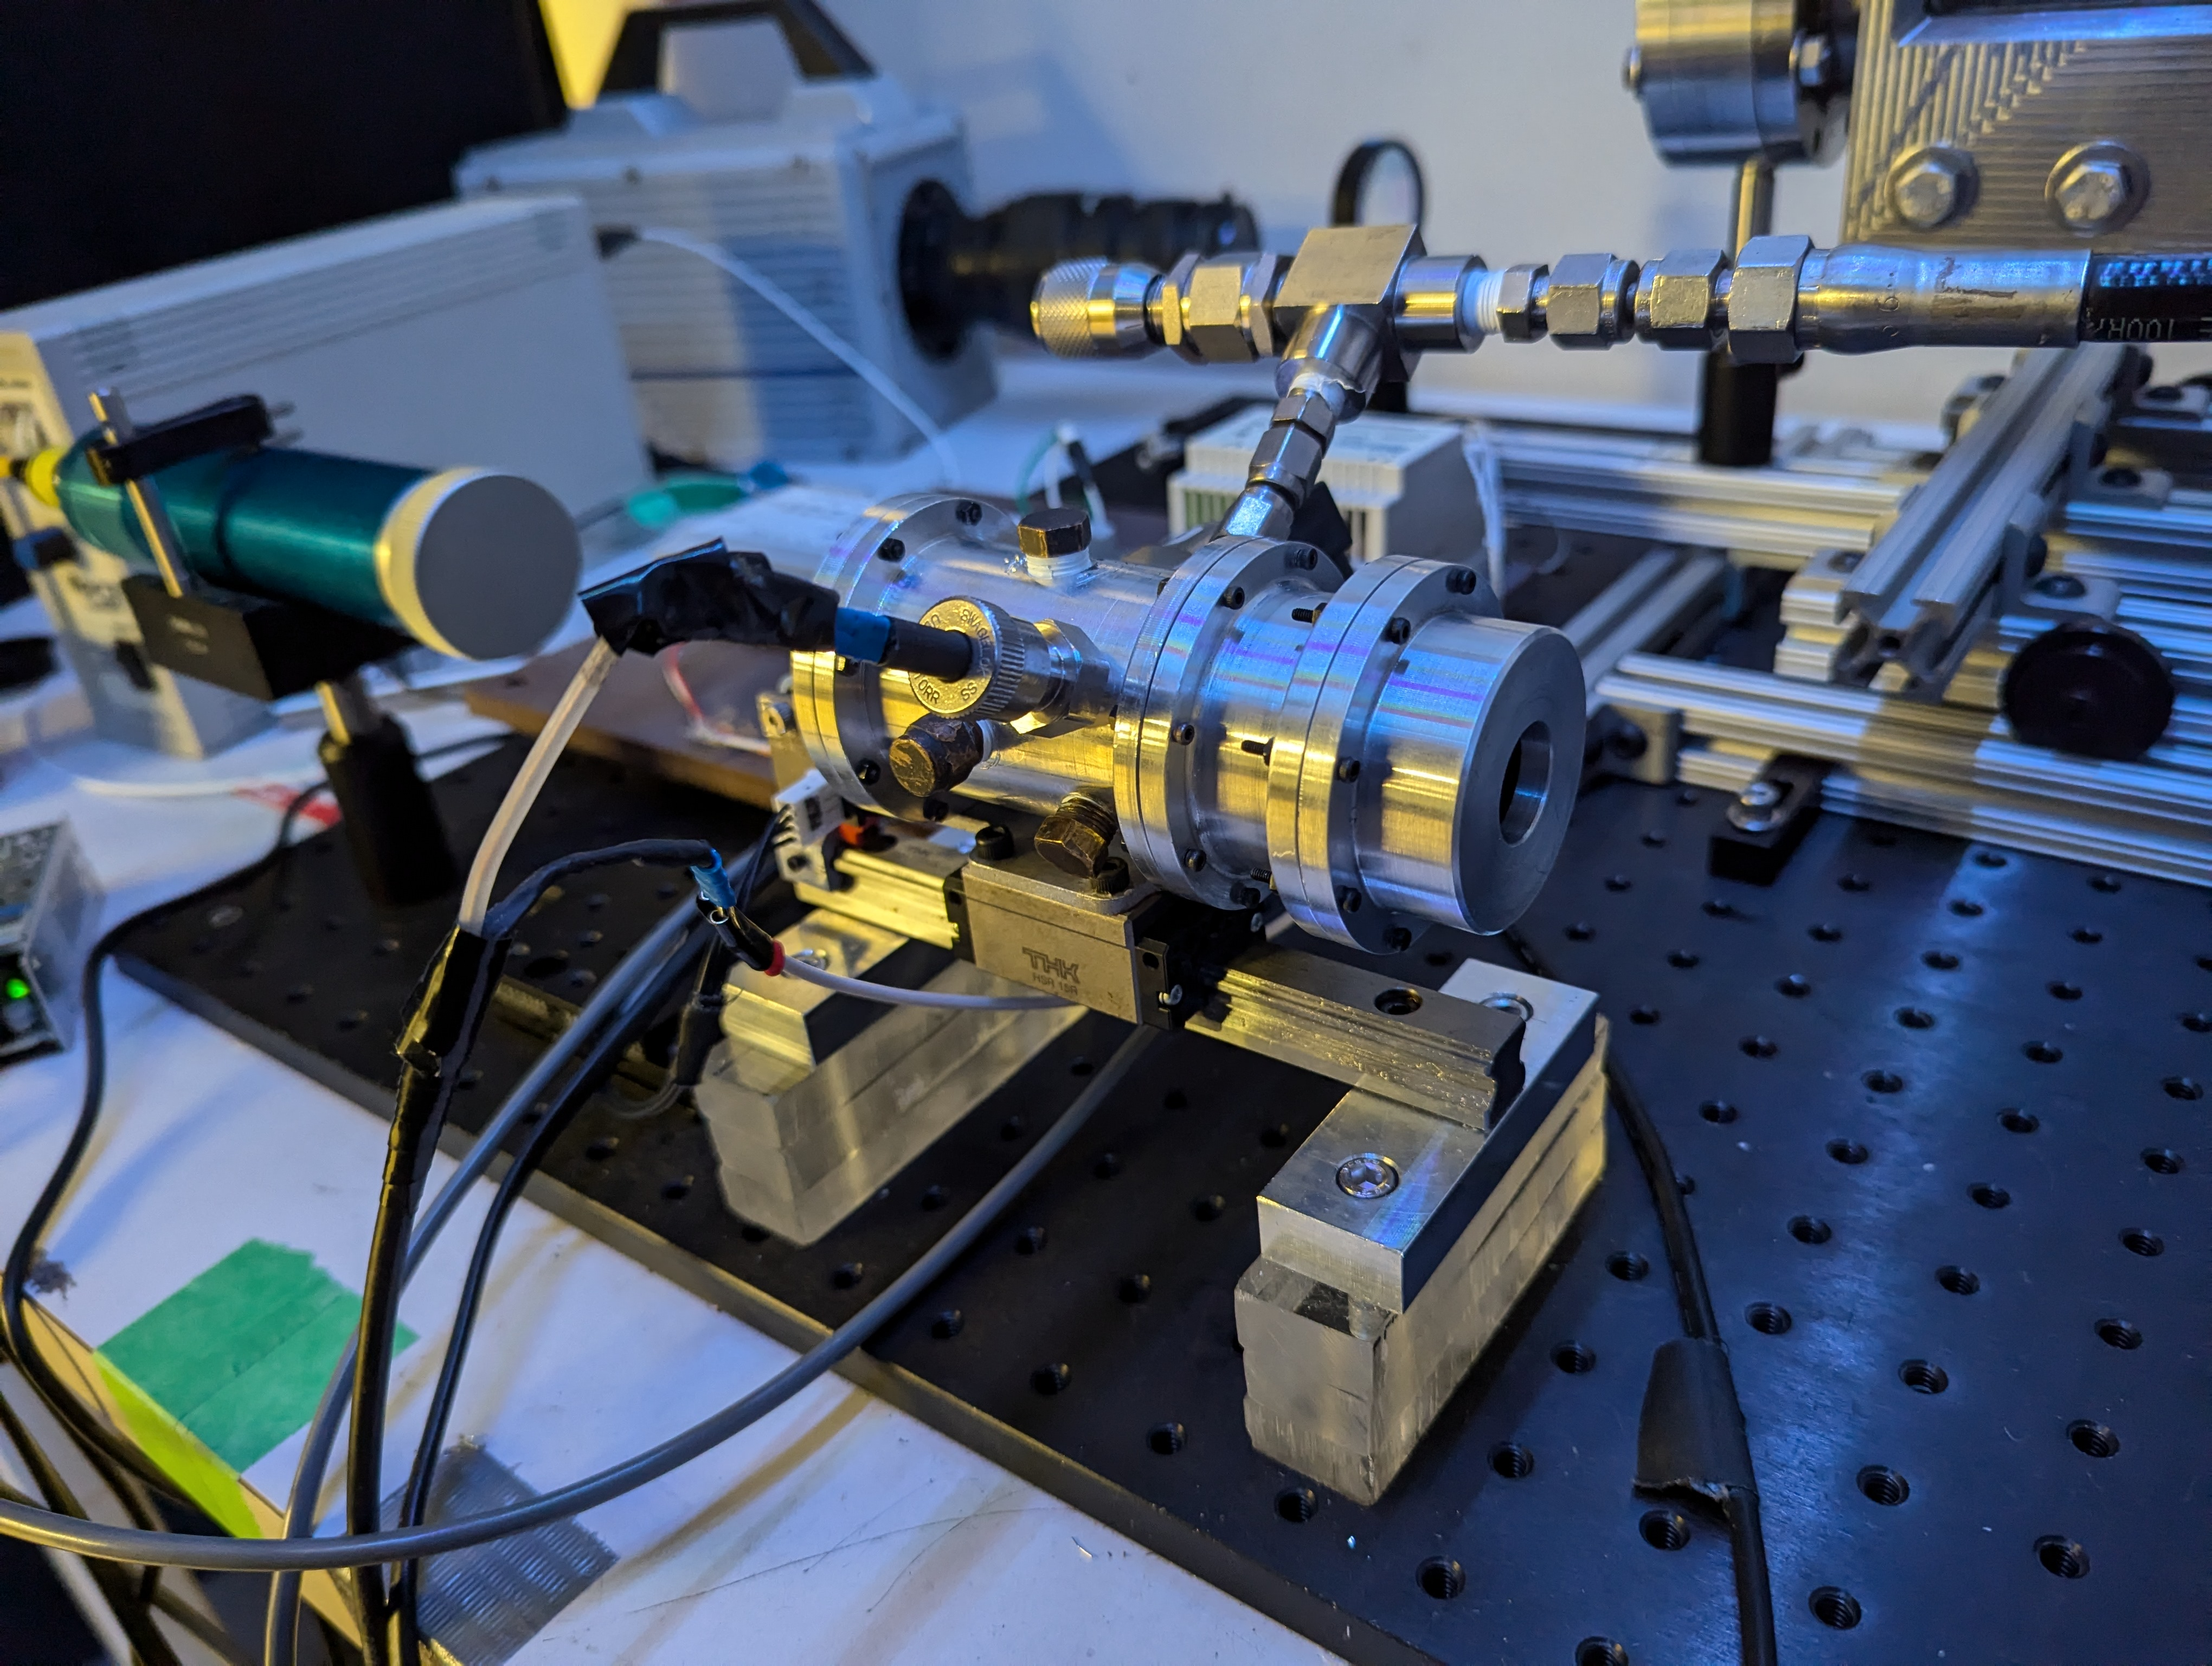
\includegraphics[width=\textwidth]{assets/3 design/V2 Static configuration.jpg}
                    \caption{Static configuration. Note the extension part and window mount.}
                \end{subfigure}
                \hfill
                \begin{subfigure}[t]{0.45\textwidth}
                    \centering
                    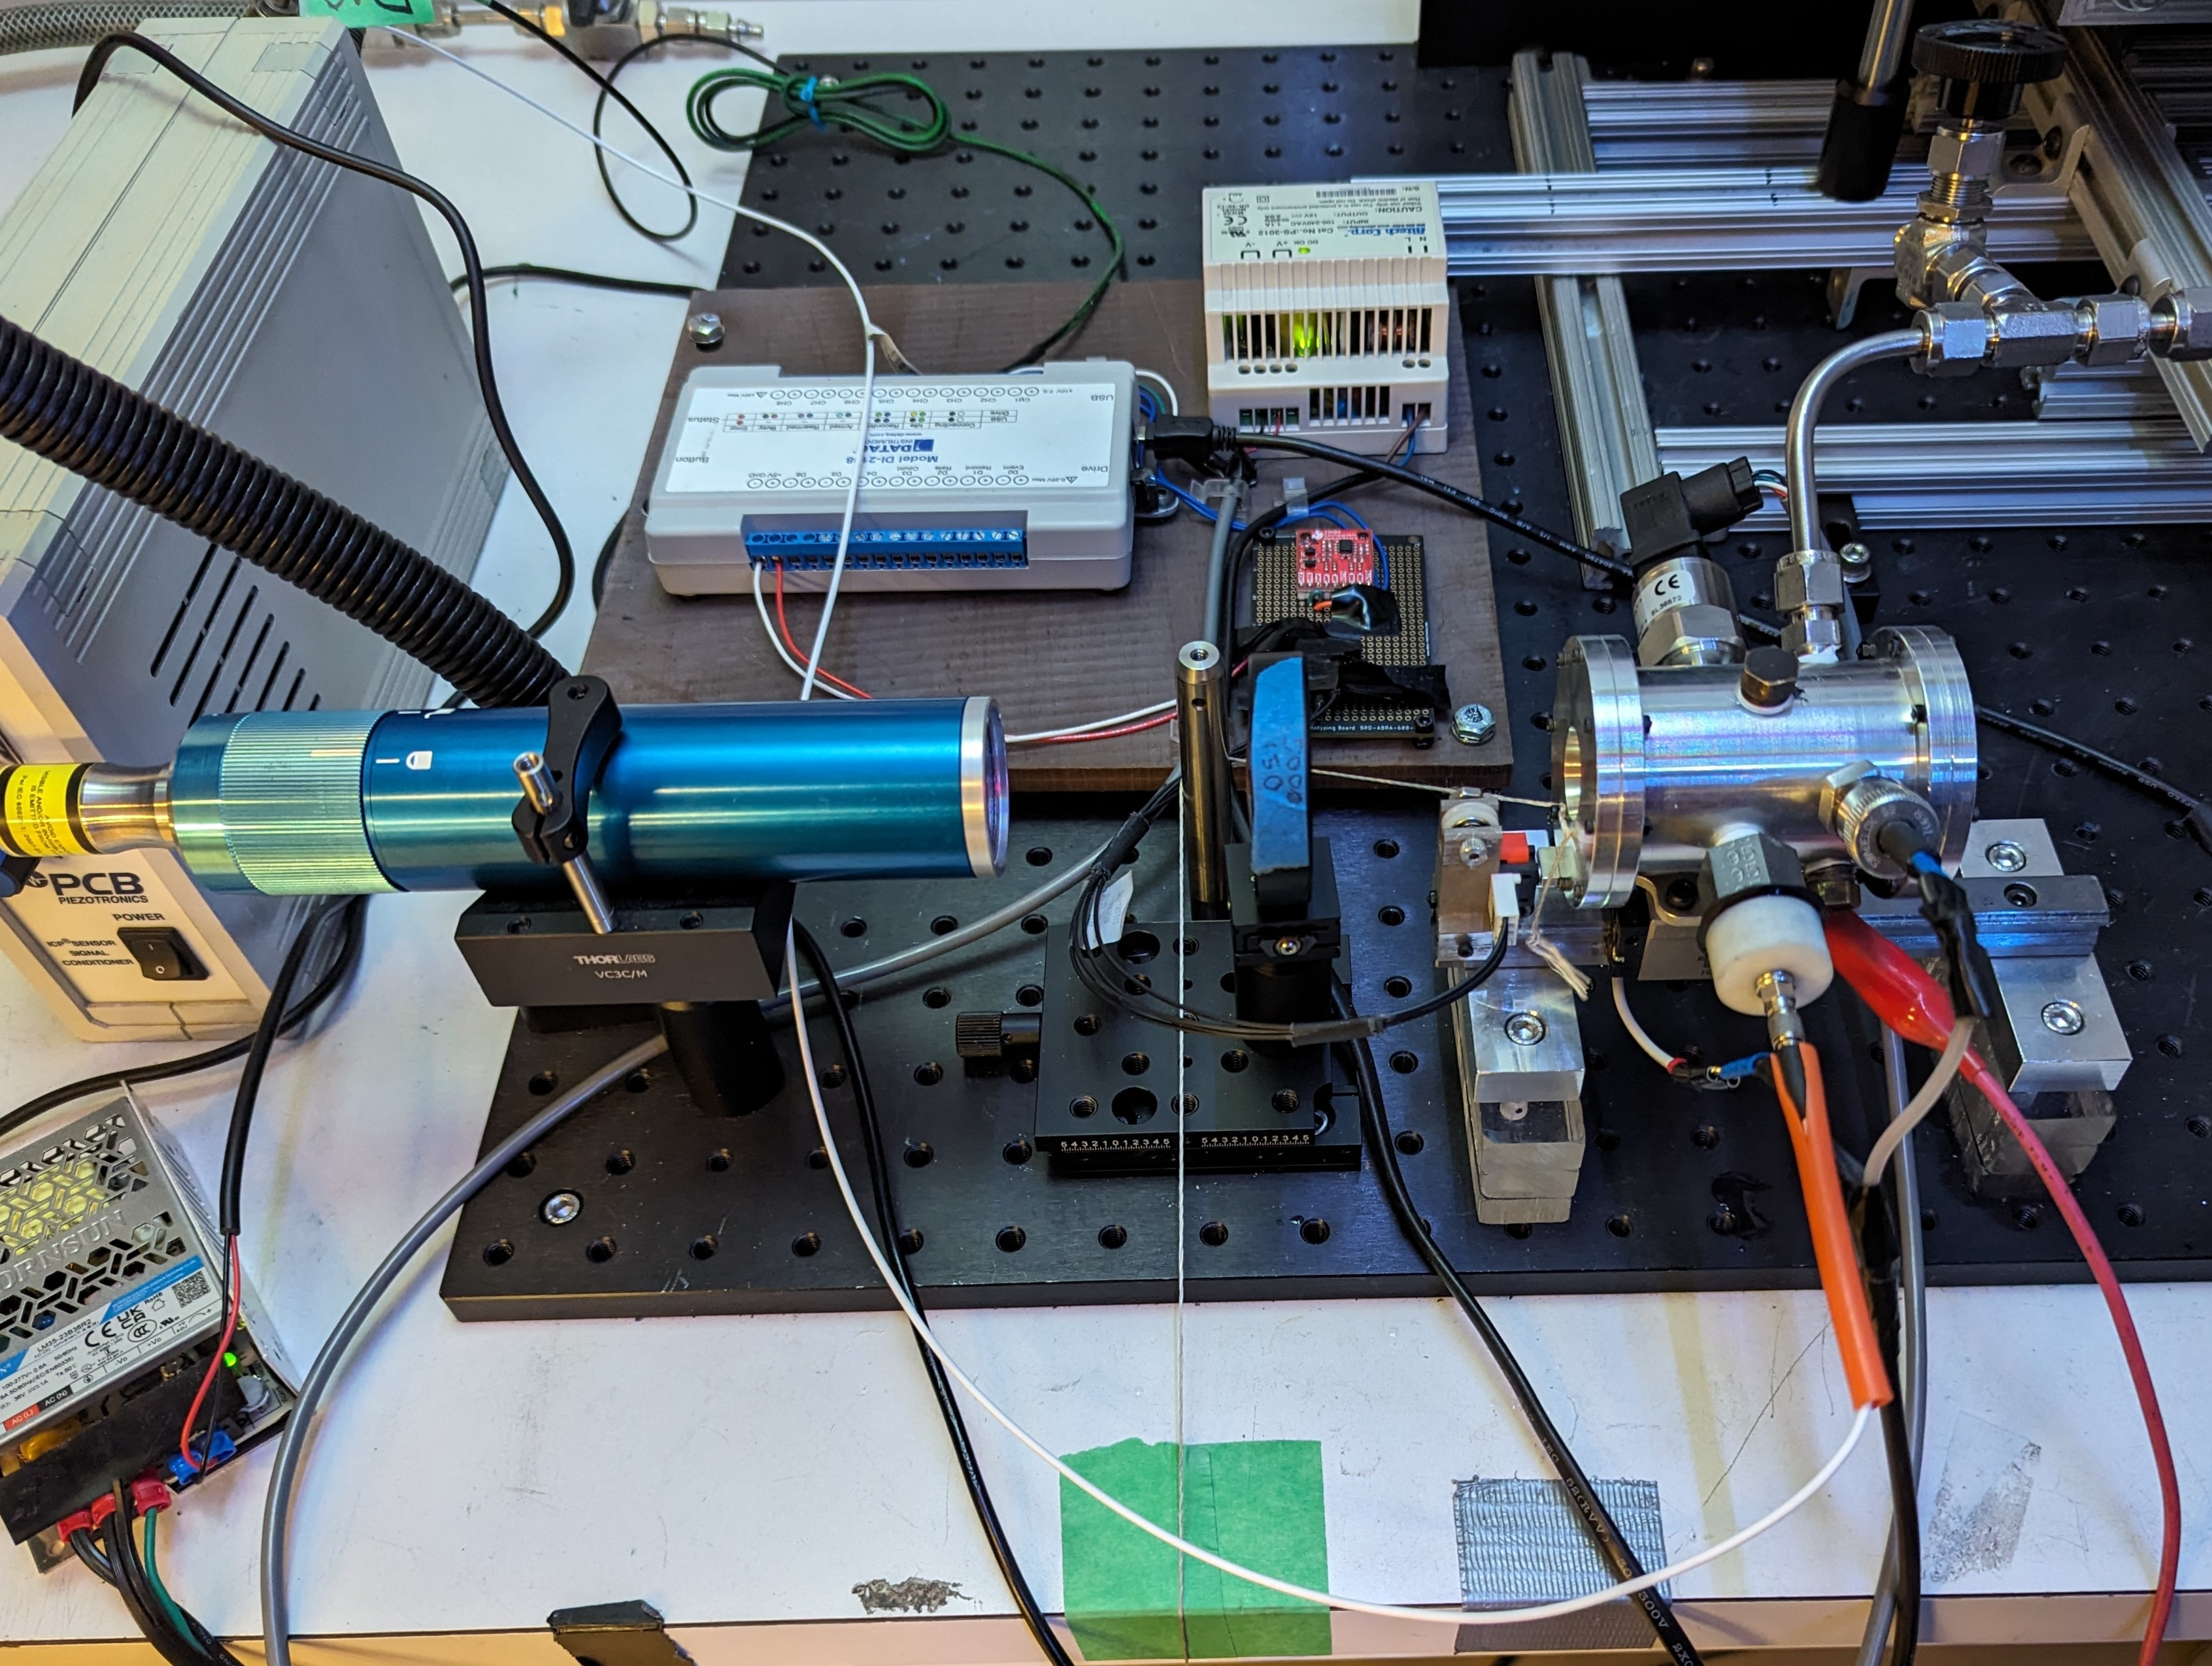
\includegraphics[width=\textwidth]{assets/3 design/V2 flowing setup.jpg}
                    \caption{Flowing configuration. The nozzle is held by the rear plate.}
                \end{subfigure}
                \caption{V2 LTP thruster}
                \label{fig:V2 setup}
            \end{figure}

            The thrust stand is a ball bearing carriage (McMaster-Carr 6709K12) mounted on a \qty{15}{mm} wide rail (McMaster-Carr 6709K33). A string through a pulley holds a variable weight, adding a preload to the test section. This ensures adequate contact between the test section and the load cell. Two load cells are used with different force sensing range: Honeywell FSG020WNPB (\qtyrange{0}{20}{N}) and Honeywell FSG005WNPB (\qtyrange{0}{5}{N}).

        \subsection{Laser}

            The laser used as the plasma's power source is an IPG Photonics YLR-300/3000-QCW-MM-AC Ytterbium fiber laser. The wavelength of the emitted light is \qty{1070}{nm}. Its nominal maximum power is \qty{3}{kW} quasi-continuous wave (QCW) or \qty{300}{W} continuous wave (CW). At \qty{3}{kW}, a QCW pulse has a maximum duration of \qty{10}{ms}. The maximum duration of a \qty{300}{W} QCW pulse is \qty{50}{ms} The laser light exits through an IPG Photonics P30-001736 collimator. The output beam is \qty{30}{mm} in diameter.

            \begin{figure}[!ht]
                \centering
                \begin{subfigure}[t]{0.45\textwidth}
                    \centering
                    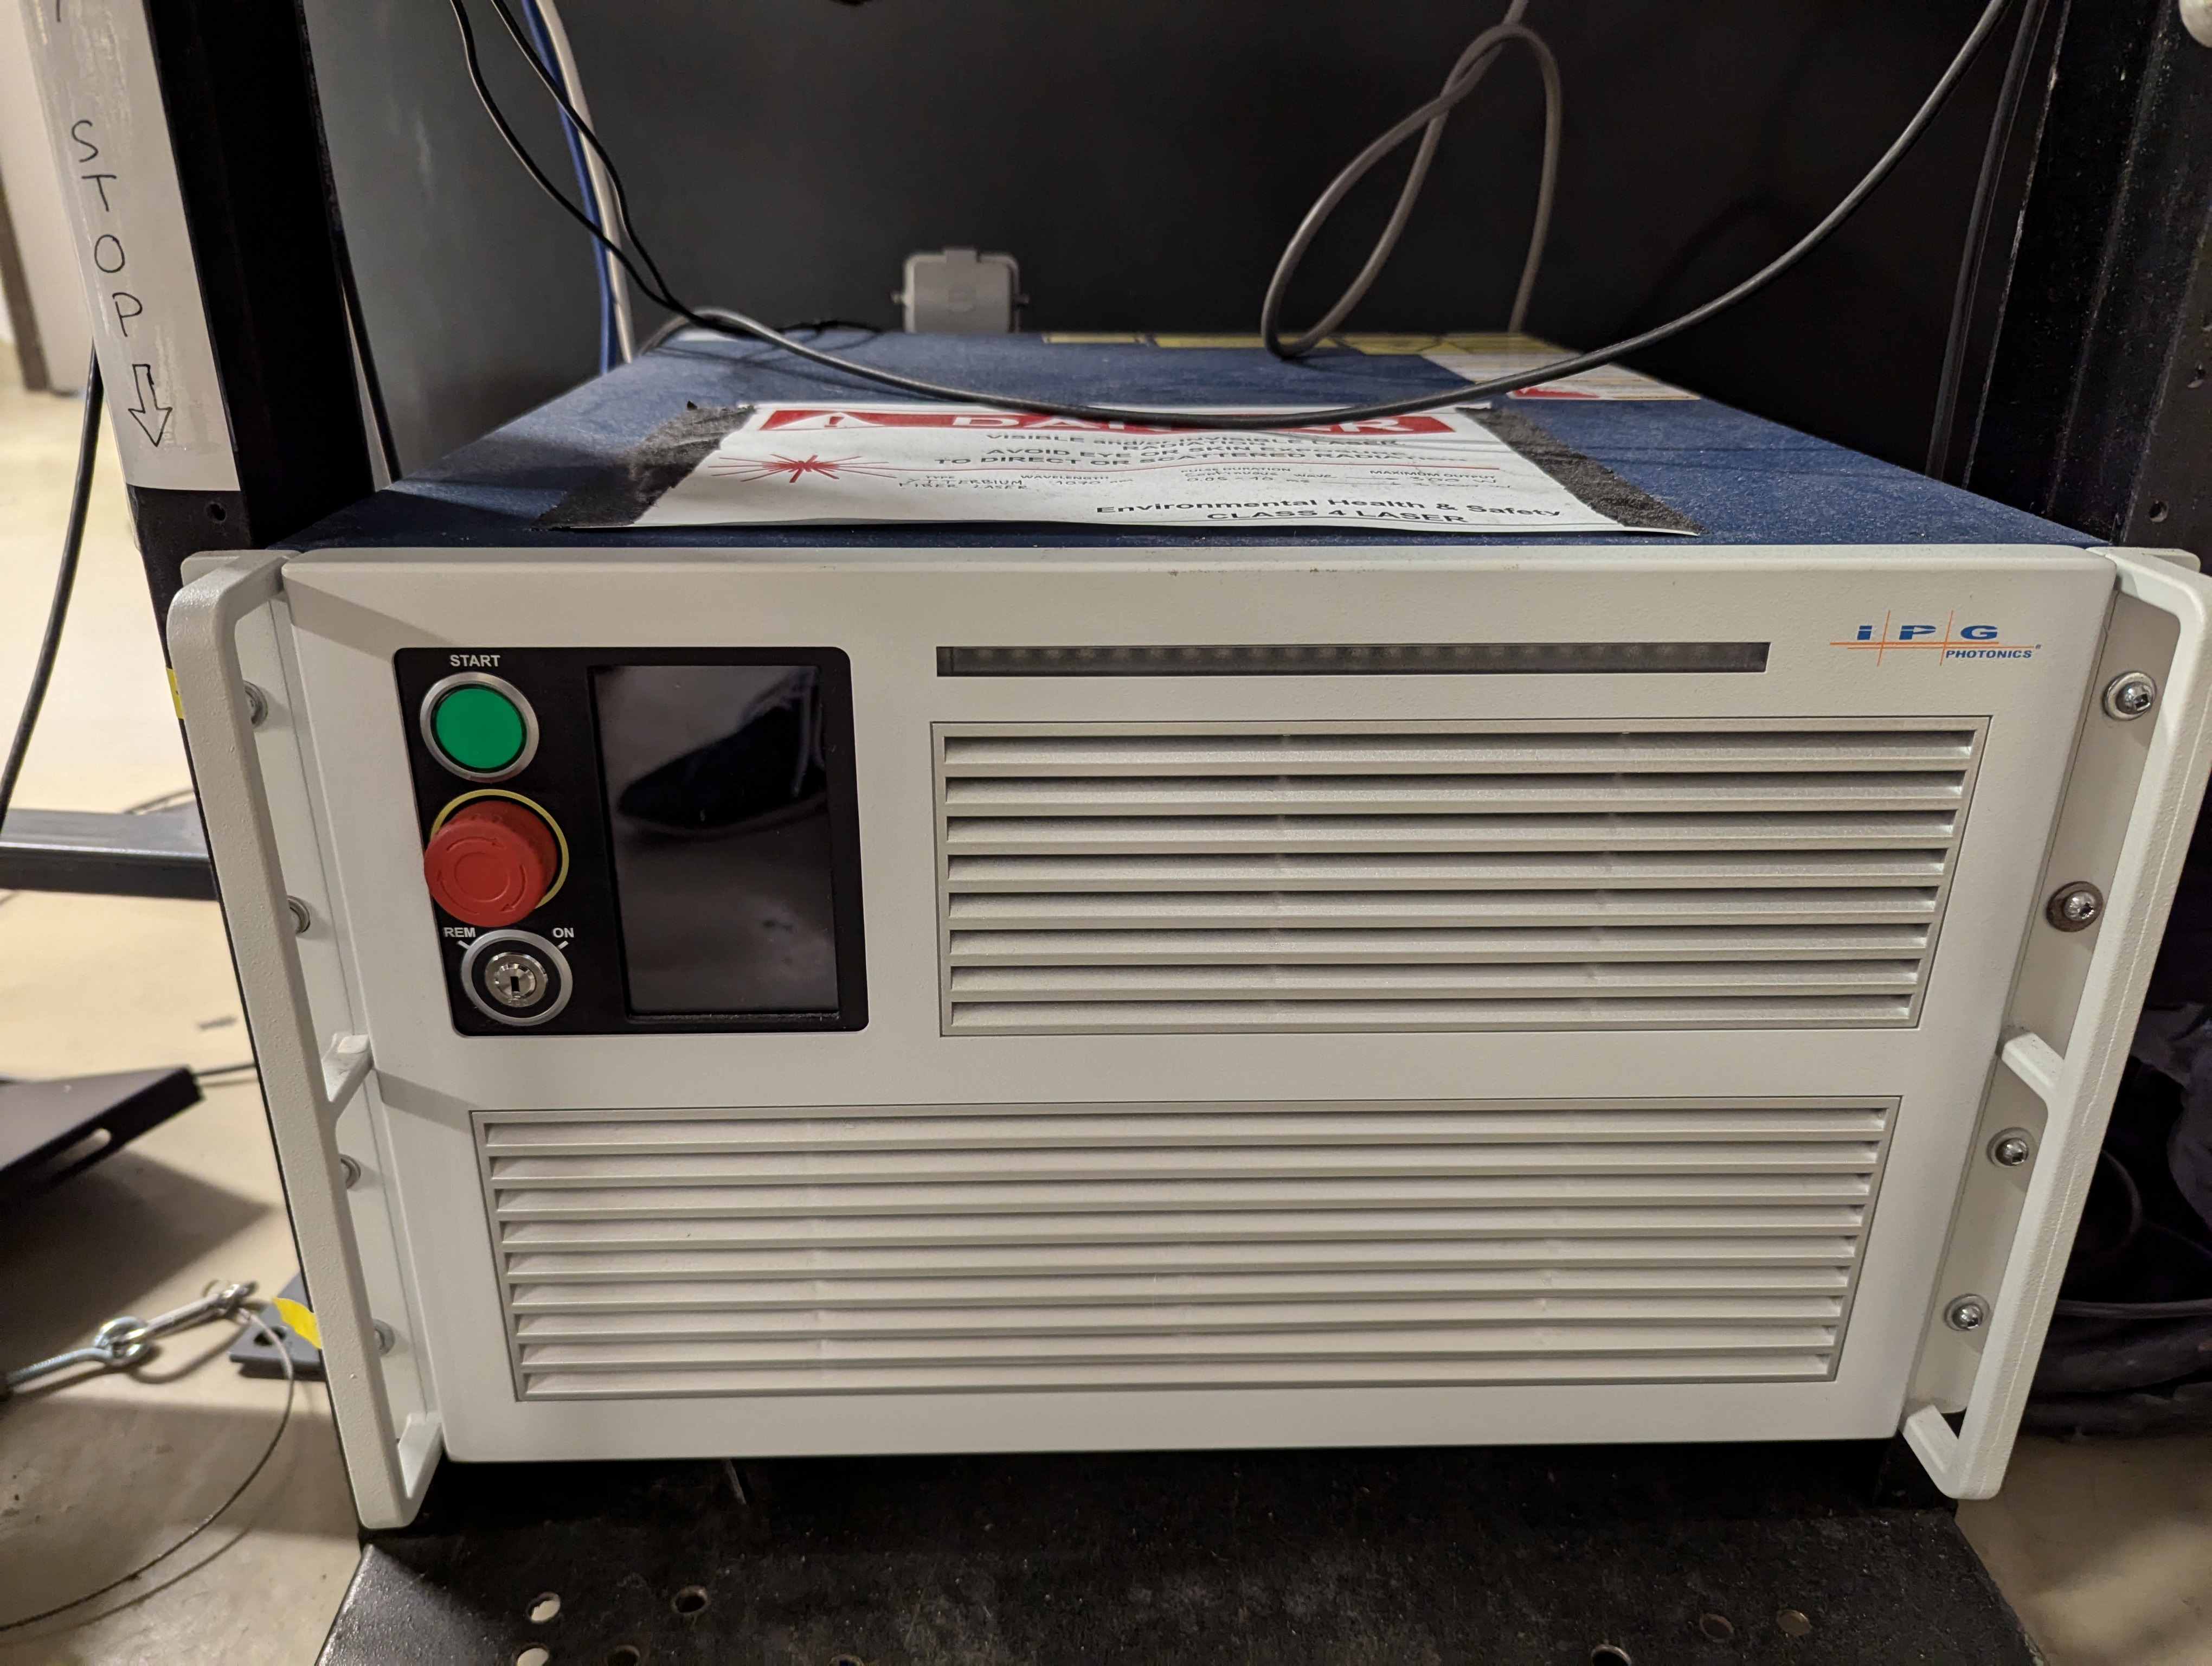
\includegraphics[width=\textwidth]{assets/3 design/Laser box.jpg}
                    \caption{IPG Photonics YLR-300/3000-QCW-MM-AC laser}
                \end{subfigure}
                \hfill
                \begin{subfigure}[t]{0.45\textwidth}
                    \centering
                    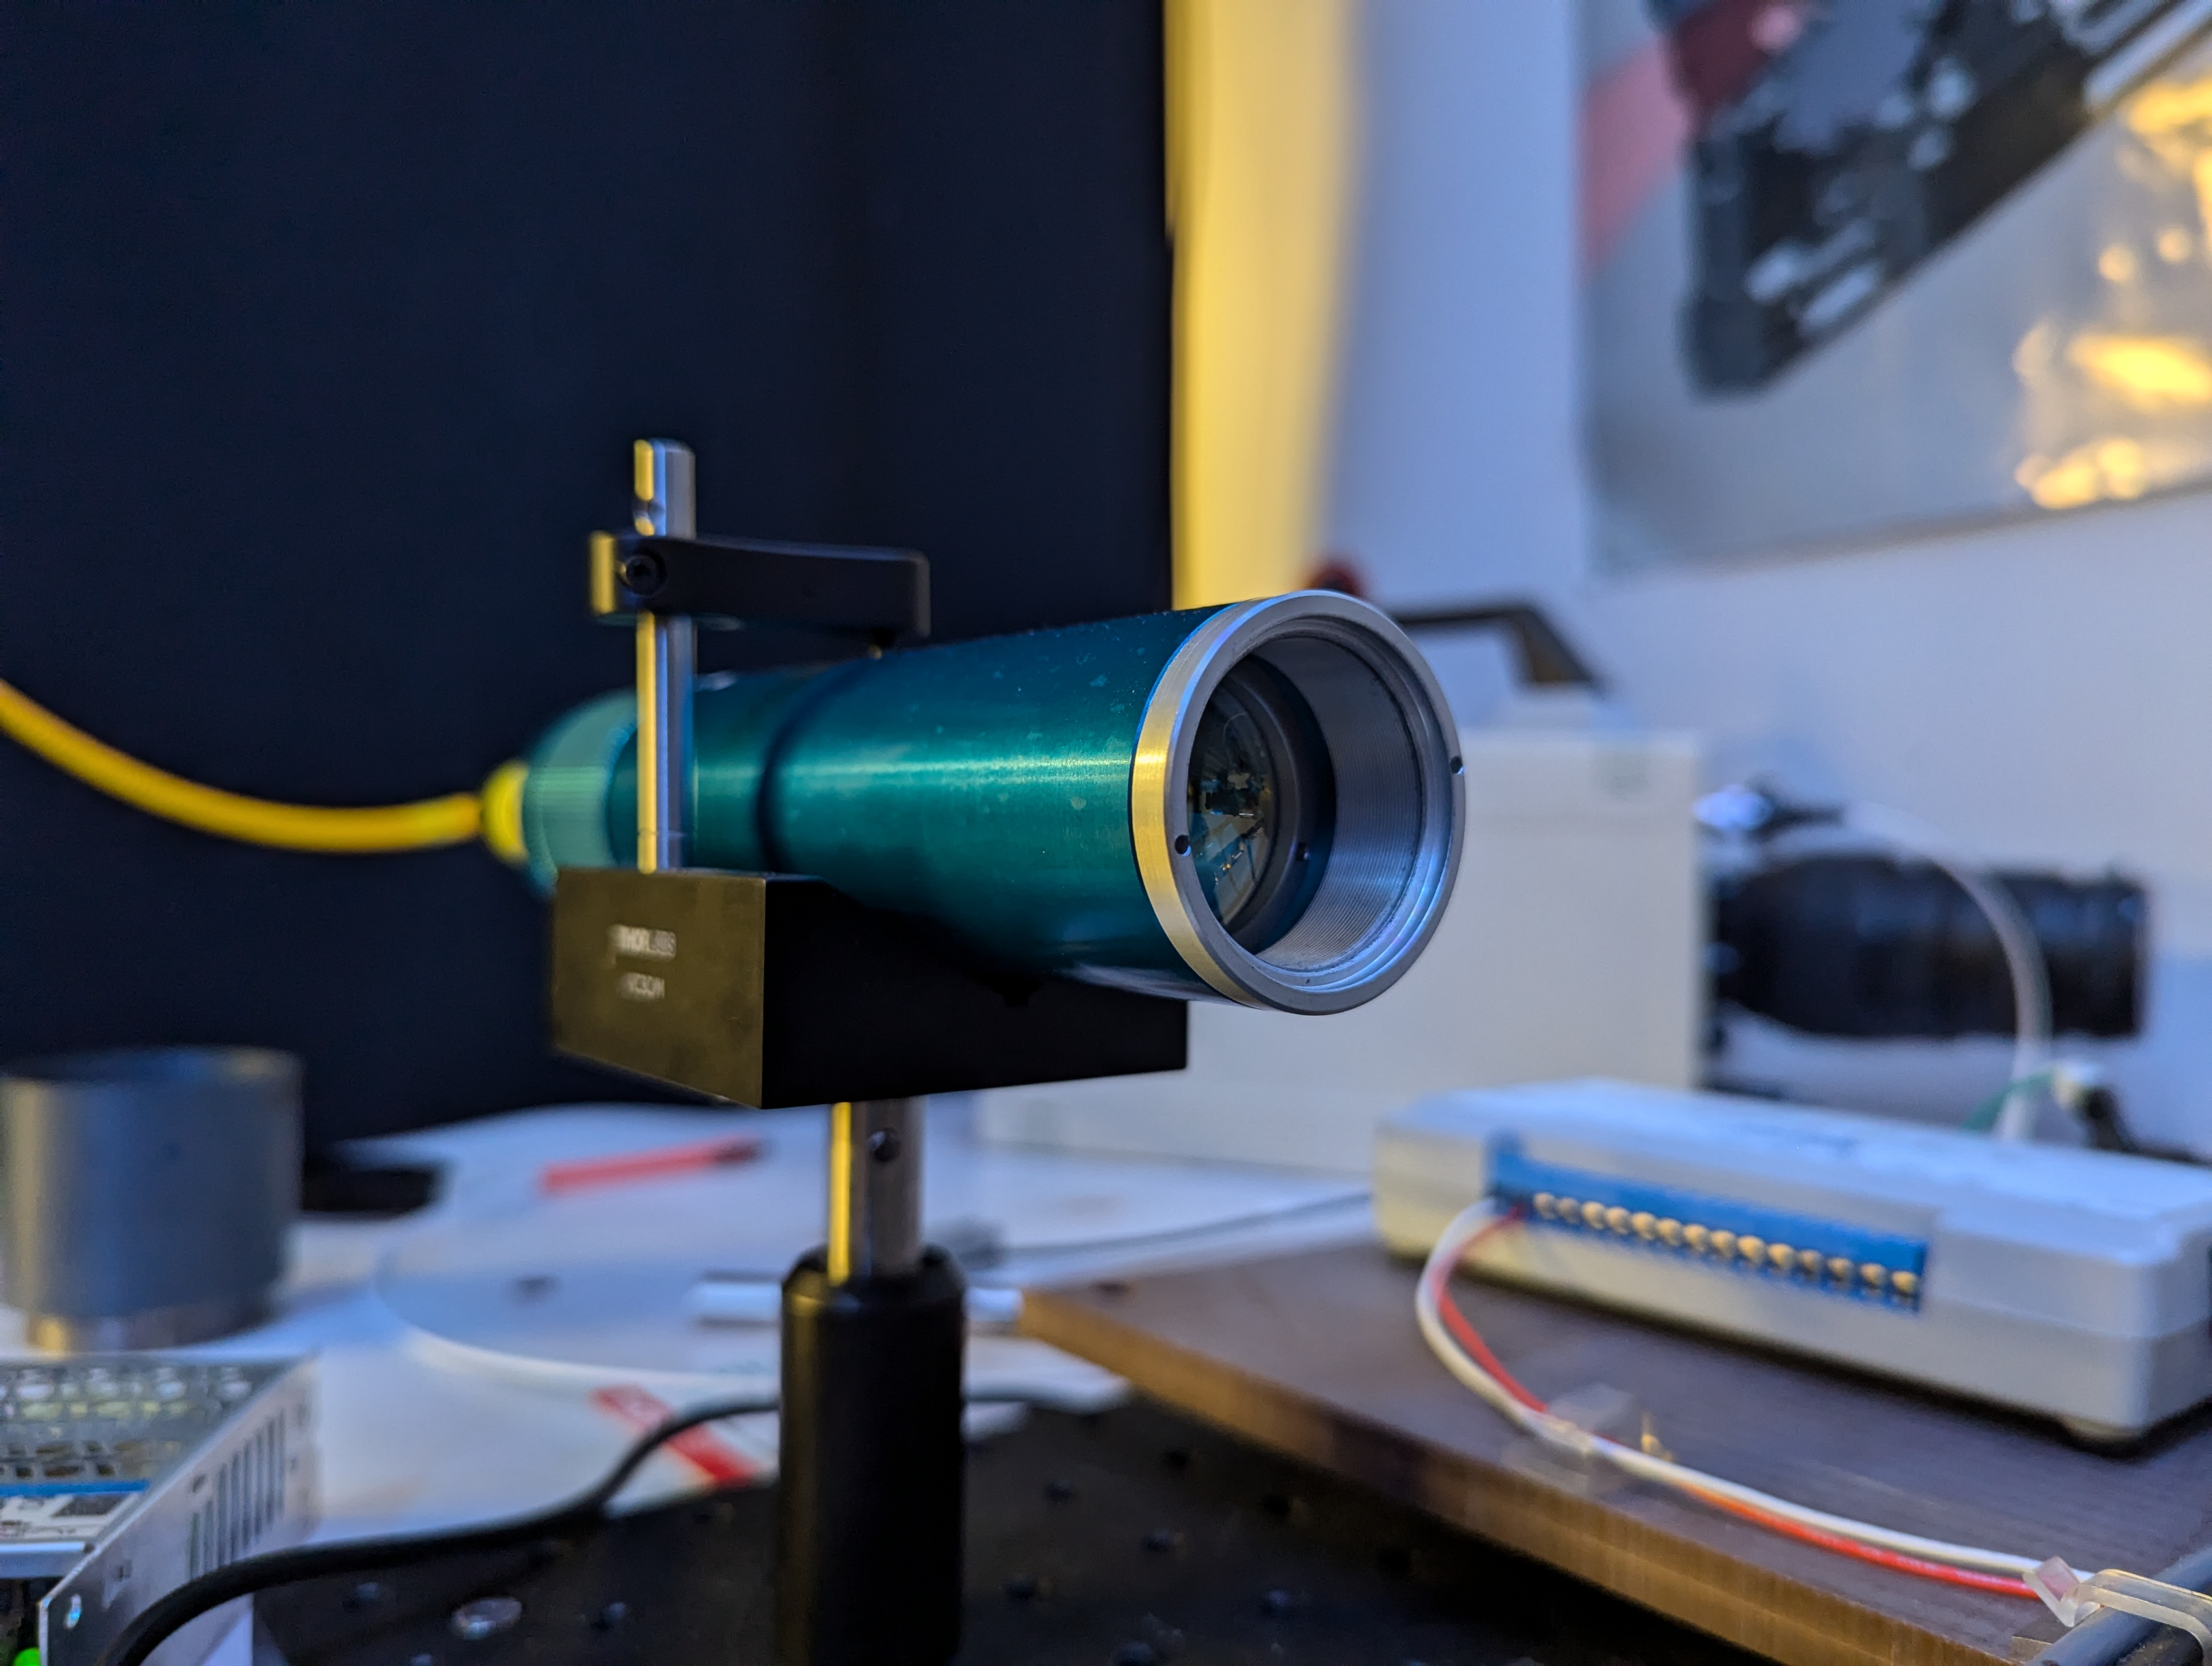
\includegraphics[width=\textwidth]{assets/3 design/Laser aperture.jpg}
                    \caption{IPG Photonics P30-001736 collimator}
                \end{subfigure}
                \caption{Laser system}
            \end{figure}

            Calibration reports for the laser and the collimator can be found in the appendix. [ADD TO APPENDIX]

        \subsection{Spark initiation system}

            AEM coil and electronics box.

        \subsection{Timing control}

            Correct timing of the laser and spark initiation is necessary to initiate LSP when the laser is in QCW mode, and to minimize damage to V2's nozzle in CW mode. To this end, delay generators are used (BNC models 7010 and 7055).

        \subsection{Data acquisition (DAQ) system and oscilloscope}

            Load cell and pressure transducer voltage is sent to a DATAQ Instruments DI-2018. This data is streamed to a personal computer by USB, where the thrust and pressure traces can be saved for analysis. Two pressure sensors were used: [PCB and OMEGA]

            \begin{figure}[!ht]
                \centering
                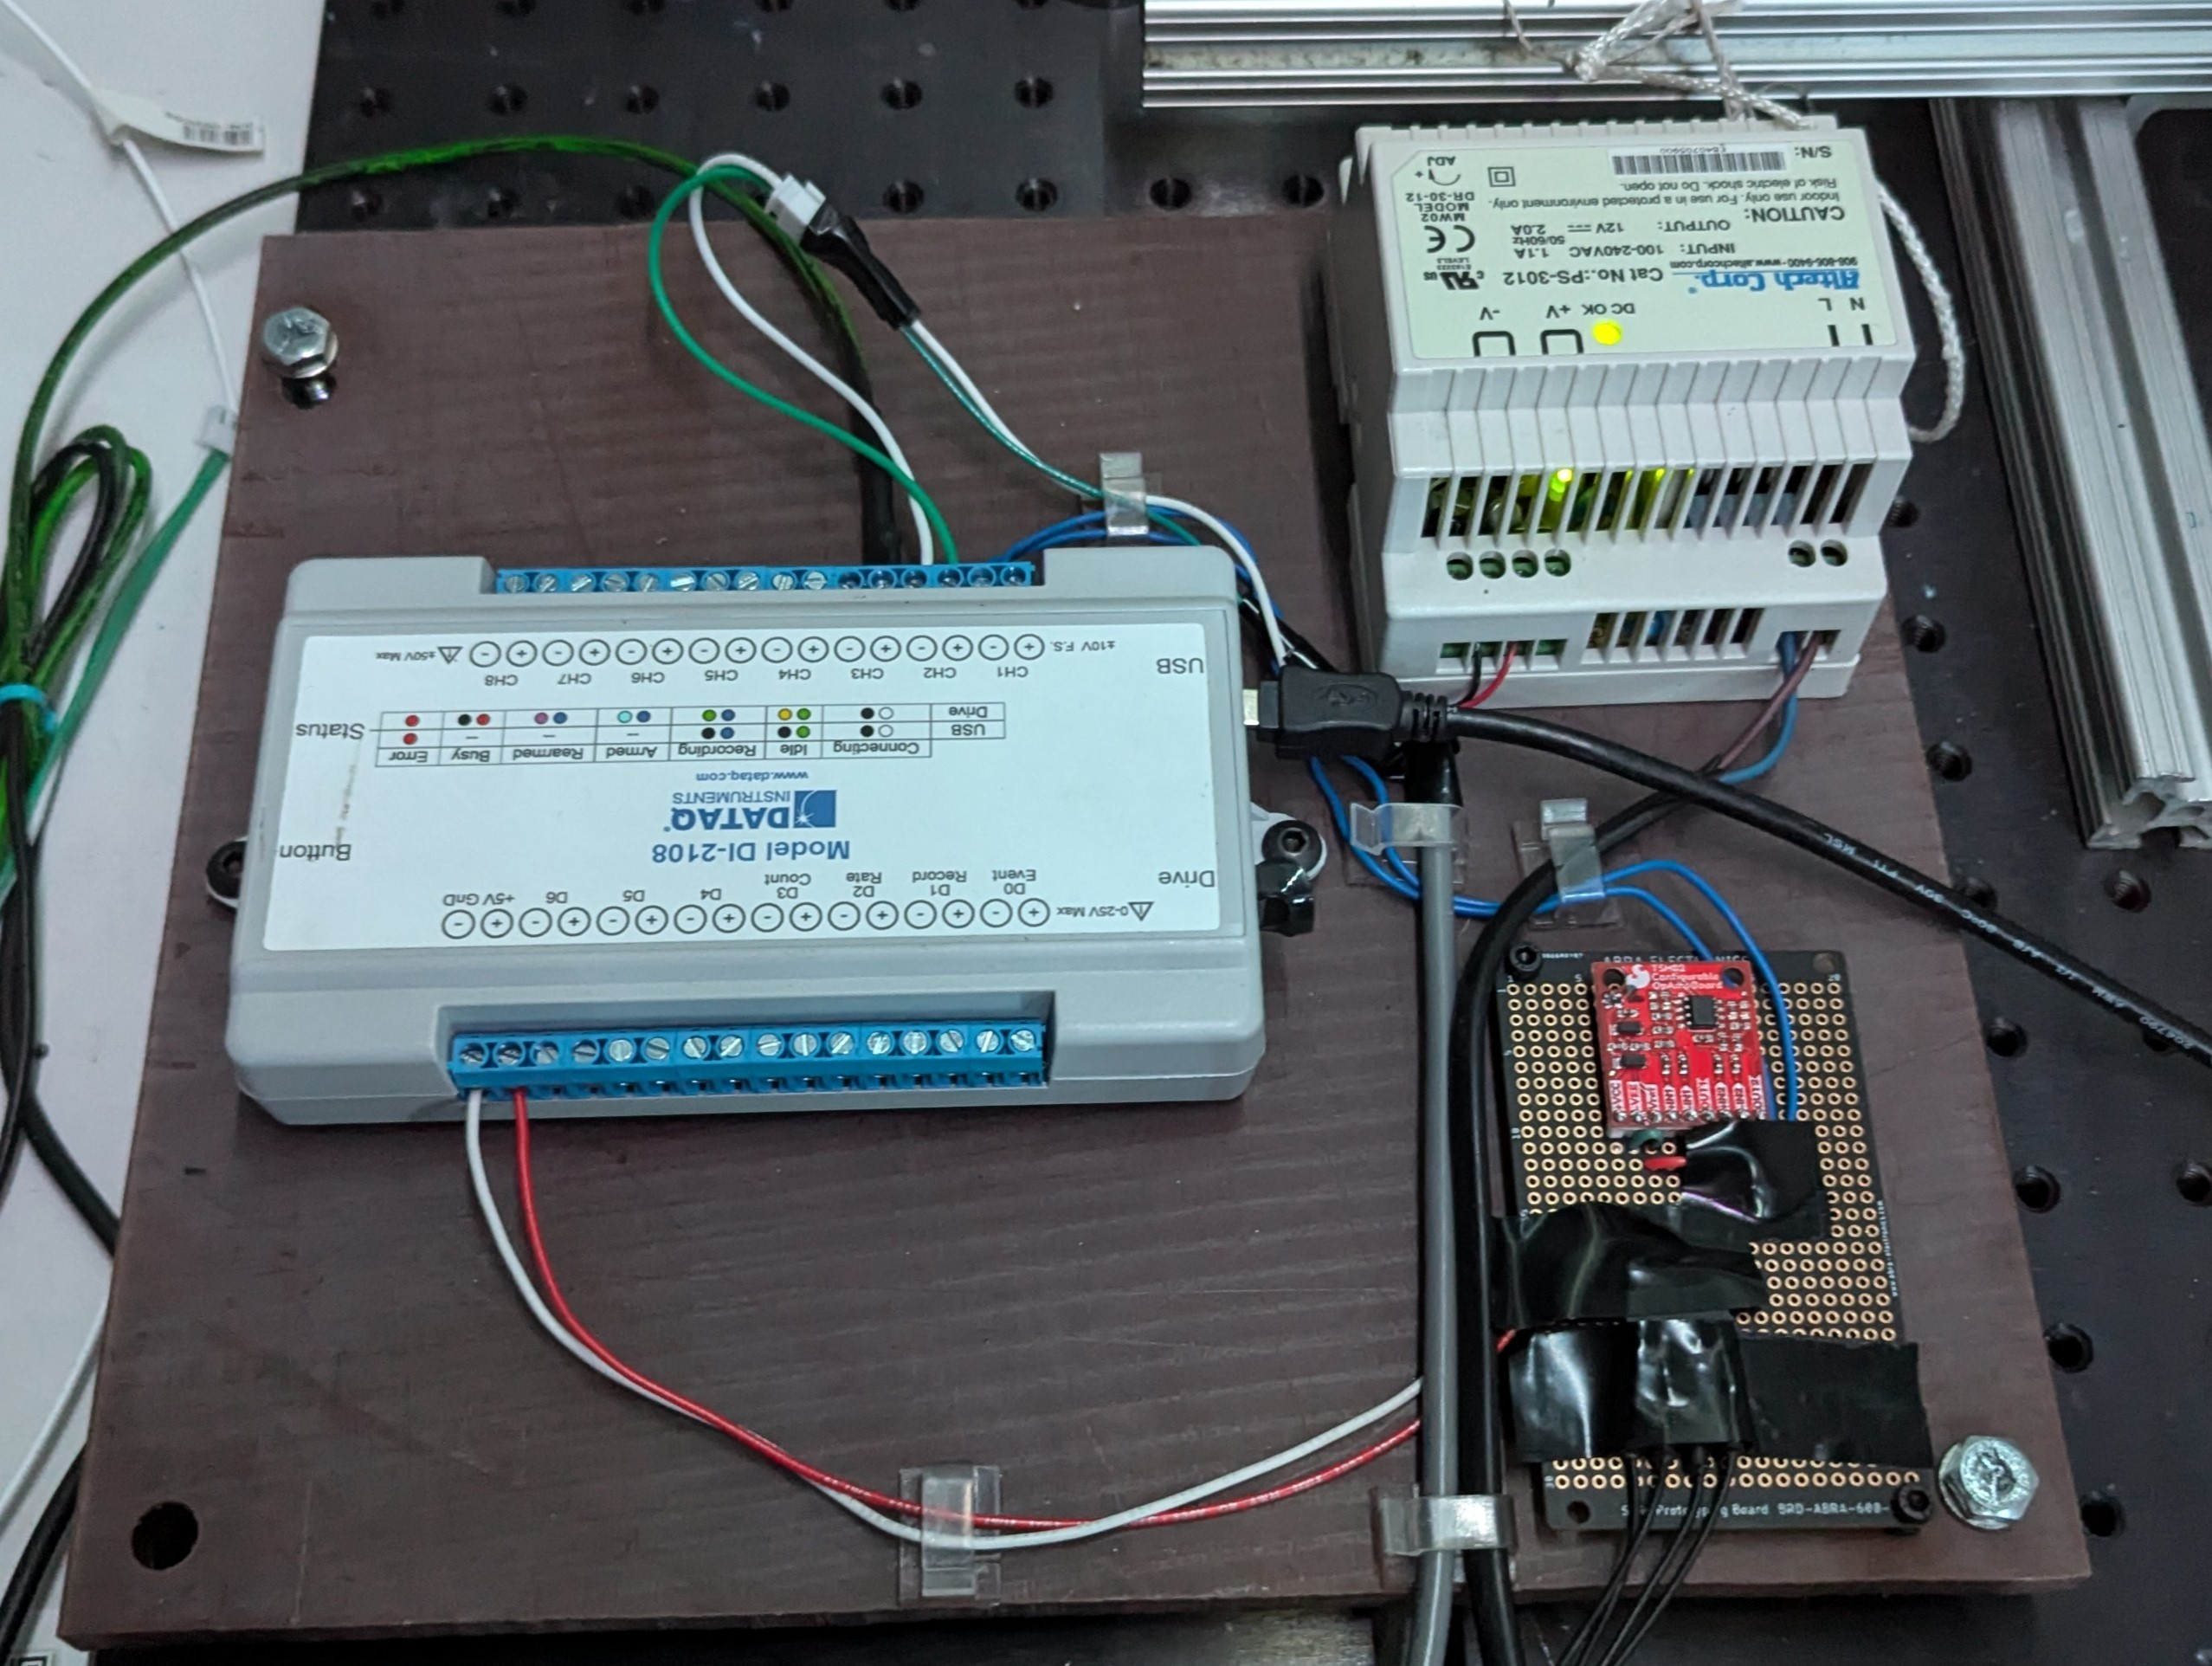
\includegraphics[width=0.50\textwidth]{assets/3 design/DAQ electronics.jpg}
                \caption{DAQ system}
                \label{fig:DAQ}
            \end{figure}

            [Photos of pressure sensor and PCB assembly]

        \subsection{High speed camera}

            A Photron SA5 high speed camera was used on certain LSP shots to validate 
            
            Due to the fact that no side window was present on V2, the Photron SA 5 high speed camera looking into the core of the thruster was used to validate.

            [Photo of Photron looking into thruster]
    \chapter{Modelling} \label{chp:models}
    Although the work of this project was primarily experimental, some modelling work was performed in order to better understand the physics of LSP and aid in the experimental design. One major area of interest is in determining the absorption properties of LSP. High laser absorption is desirable to maximize power conversion efficiency. Furthermore, the IB absorption coefficient typically reaches a maximum at a specific temperature. According to \textcite{keeferLaserSustainedPlasmas1989}, this peak absorption temperature was found to closely correlate with LSP peak temperature. The measurement of absorption coefficient can thus be used to support LSP temperature estimates.

    \section{Absorption} \label{sec:models_absorption}
        A critical property of LSP is its ability to absorb laser radiation. As stated in \autoref{sec:background_lsp}, the primary mechanism for radiation absorption in LSP is inverse bremsstrahlung. Calculation of the absorption coefficient of this process is critical for modelling LSP behavior and estimating its laser absorption efficiency. The calculation method presented here aims to adapt the work of \textcite{akarapuNumericalModelLasersustained2009,nassarInvestigationLasersustainedPlasma2012}, who have developed CFD models for the use of Argon LSP in surface-treatment applications. Although their work considered \ce{CO_2} lasers, adapting the method to the fiber laser of this study is a matter of using the appropriate laser frequency in \autoref{eq:ib_absorption}. Their work was thus used to validate each calculation step, and their results will be plotted alongside this study's computations when relevant.
        
        The absorption coefficient can be calculated using \autoref{eq:ib_absorption} and is heavily dependent on electron density $n_\mathrm{e}$ and radiation frequency $\nu$. The first step of absorption modelling is thus to determine electron density, which is variable with temperature $T$ according to the Saha ionization equation, developed by \textcite{sahaPhysicalTheoryStellar1997}. It is reproduced here for the single ionization case as \autoref{eq:saha}:
        \begin{equation}
            \frac{n_\mathrm{e}^2}{n_0-n_\mathrm{e}} = \frac{n_\mathrm{e}^2}{n_\mathrm{Ar}} = \frac{2}{\Lambda_\mathrm{th}^3}\frac{\mathcal{Z}_{\mathrm{Ar}^+}}{\mathcal{Z}_\mathrm{Ar}}\exp{\left(-\frac{E_\text{ion, Ar}}{k_\mathrm{B}T}\right)}
            \label{eq:saha}
        \end{equation}
        Where $n_0$ is the initial number density of neutral atoms, $n_\mathrm{Ar}$ is the number density of un-ionized atoms at a given temperature, $E_\text{ion, Ar}$ is Argon's first ionization energy (\qty{15.76}{eV}), and $k_\mathrm{B}$ is the Boltzmann constant. The thermal DeBroglie wavelength $\Lambda_\mathrm{th}$ is a function of temperature as follows, where $\hbar$ is the reduced Planck constant and $m_\mathrm{e}$ is the mass of an electron:
        \begin{equation*}
            \Lambda_\mathrm{th} = \sqrt{\frac{2\pi \hbar^2}{m_\mathrm{e}k_\mathrm{B}T}}
        \end{equation*}
        The ratio $\mathcal{Z}_{\mathrm{Ar}^+}/\mathcal{Z}_\mathrm{Ar}$ is the ratio of the partition function values for Ar$^+$ and Ar (also designated Ar II and Ar I, respectively). These values are also dependent on temperature and can be queried in the NIST Atomic Spectra Database (\textcite{kramidaNISTAtomicSpectra2022}) for a given spectrum (e.g., Ar I) and electron temperature $T_\mathrm{e}$. This ratio is plotted in \autoref{fig:e_density_partition}. \citeauthor{nassarInvestigationLasersustainedPlasma2012} fitted a seventh-order polynomial to approximate this ratio across temperature, which is also plotted for comparison.

        It is important to note that $n_0$ in \autoref{eq:saha} is not constant across temperatures. In the case of LSP, the ionization process occurs at constant pressure, even if the experiment occurs in a closed container, as only a small fraction of the test section volume undergoes ionization. The hotter Argon is free to expand into the cooler surroundings, locally reducing the number density and maintaining a constant pressure. Therefore, $n_0$ must be calculated based on a given pressure $p$ and the varying temperature. This can be done with the ideal gas equation, where $V$ is volume, $N$ is the number of atoms in moles, $R_\mathrm{u}$ is the universal gas constant, and $N_\mathrm{A}$ is Avogadro's number:
        \begin{align*}
            pV&= NR_\mathrm{u}T \\
            p&= \frac{N}{V}R_\mathrm{u}T \\
            \frac{N_\mathrm{A}p}{R_\mathrm{u}T}&= n_0
        \end{align*}

        The electron density $n_\mathrm{e}$ is plotted against temperature in \autoref{fig:e_density_curves}, for a pressure of \qty{1}{bar}. The calculation by \citeauthor{nassarInvestigationLasersustainedPlasma2012} is plotted alongside it, and their relative value is compared. While the electron density plots appear to agree, there remains a difference in density of a factor of two. This appears to be due to the use of lower precision physical constants in \citeauthor{akarapuNumericalModelLasersustained2009} and \citeauthor{nassarInvestigationLasersustainedPlasma2012}'s work.

        \begin{figure}[h]
            \centering
            \begin{subfigure}[t]{2.6in}
                \centering
                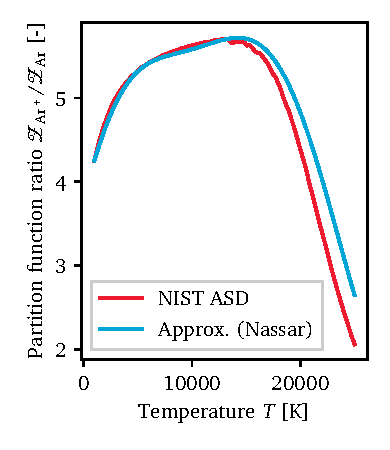
\includegraphics[]{assets/4 models/partition}
                \caption{Ratio of Ar II to Ar I partition function values}
                \label{fig:e_density_partition}
            \end{subfigure}
            \hfill
            \begin{subfigure}[t]{3.2in}
                \centering
                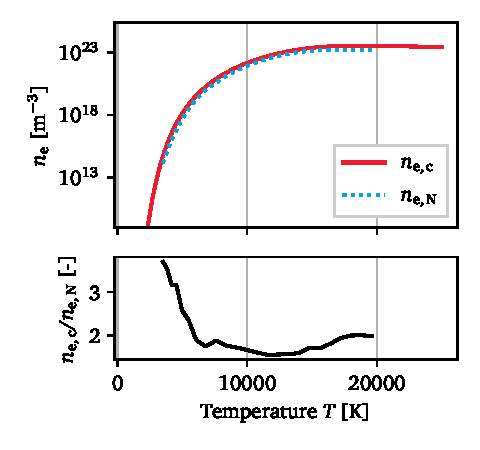
\includegraphics[]{assets/4 models/n_e}
                \caption{$n_e$ at \qty{1}{bar}, and comparison between computed density $n_\mathrm{e, c}$ and density $n_\mathrm{e, N}$ reported by \textcite{nassarInvestigationLasersustainedPlasma2012}}
                \label{fig:e_density_curves}
            \end{subfigure}
            \caption{Computation of electron density $n_\mathrm{e}$ of Argon}
            \label{fig:e_density}
        \end{figure}

        Although electron density appears to plateau past \qty{20000}{K}, the caveat of this calculation is that it only considers single-ionization. While this is valid below \qty{20000}{K}, second-degree ionization begins past this temperature. The plot is extended up to \qty{25000}{K} to provide some estimate of plasma properties, although they will not be as accurate as below \qty{20000}{K}.

        The absorption coefficient $\alpha$ can now be calculated with the known electron density. For convenience, the equation for $\alpha$, \autoref{eq:ib_absorption}, is reproduced here:
        \begin{equation*}
            \ibalphaeq \tag{\ref{eq:ib_absorption} revisited}
        \end{equation*}
        Most parameters have been defined in \autoref{sec:background_lsp}, so the Coulomb logarithm $\ln{\Lambda}$ and the plasma frequency $\nu_\mathrm{p}$ will be of interest here. The Coulomb logarithm is evaluated by \textcite{nassarInvestigationLasersustainedPlasma2012} using a common approximation seen in plasma physics (\textcite{richardson2019NRLPlasma2019}):
        \begin{equation}\label{eq:coulombLog_NRL}
            \ln{\Lambda} \approx 23-\ln{(n_\mathrm{e}^{1/2}ZT_\mathrm{e}^{-3/2})}
        \end{equation}
        However, alternate evaluations of the logarithm exist, such as the one given by \textcite{johnstonCorrectValuesHighfrequency1973} in the specific context of IB absorption coefficient calculation (\autoref{eq:coulombLog_johnston}). 
        \begin{equation} \label{eq:coulombLog_johnston}
            \Lambda(\nu) = \begin{cases}
                \frac{v_T}{\nu\rho_\mathrm{min}} & \nu \gg \nu_\mathrm{p}\\
                \frac{v_T}{\nu_\mathrm{p}\rho_\mathrm{min}} & \text{otherwise}
            \end{cases}
        \end{equation}
        Where $v_T$ is the electron thermal velocity, $\nu$ is the laser frequency, $\nu_\mathrm{p}$ is the plasma frequency, and $\rho_\mathrm{min}$ is the impact parameter. These can be evaluated with the following equations:
        \begin{gather}
            v_T = \sqrt{\frac{k_\mathrm{B}T}{m_\mathrm{e}}} \\
            \nu_\mathrm{p} = \frac{1}{2\pi}\sqrt{\frac{e^2n_\mathrm{e}}{\epsilon_0 m_\mathrm{e}}} \approx (\qty{8.97885}{m^{3/2}s^{-1}})\sqrt{n_\mathrm{e}}\\
            \rho_\mathrm{min} \approx \max{\left(\frac{Ze^2}{k_\mathrm{B}T}, \frac{\hbar}{(m_\mathrm{e}k_\mathrm{B}T)^{1/2}}\right)}
        \end{gather}
        \textcite{johnstonCorrectValuesHighfrequency1973} state:
        \begin{quote}
            ...at frequencies well above the plasma frequency $\nu_\mathrm{p}$, $\ln{\Lambda}(\nu)$ should contain the wave frequency $\nu$ rather than the plasma frequency $\nu_\mathrm{p}$.
        \end{quote}
        The respective frequencies of the plasma, \ce{CO_2} laser, and fiber laser are plotted in \autoref{fig:coulomb_freq} for comparison. It can be seen that for a fiber-laser-powered LSP, the $\nu \gg \nu_\mathrm{p}$ case of \autoref{eq:coulombLog_johnston} is valid across the range of temperatures of interest, so \citeauthor{johnstonCorrectValuesHighfrequency1973}'s statement is highly relevant in this case, and perhaps of lesser importance in \citeauthor{nassarInvestigationLasersustainedPlasma2012}'s study. As it was not clear whether the approximation of $\ln{\Lambda}$ in \autoref{eq:coulombLog_NRL} was applicable in this case, both evaluations of the Coulomb logarithm were compared in \autoref{fig:coulomb_coulomb}, showing that while there is a large divergence at lower temperatures, this is negligible as the Argon is not in a plasma state. For temperatures of interest, namely above \qty{10000}{K}, both evaluations of the Coulomb logarithm appear to converge. \citeauthor{johnstonCorrectValuesHighfrequency1973}'s form of the logarithm was retained for further calculations as it considers the relative values of the plasma and laser frequencies.

        \begin{figure}[h]
            \centering
            \begin{subfigure}[t]{2.9in}
                \centering
                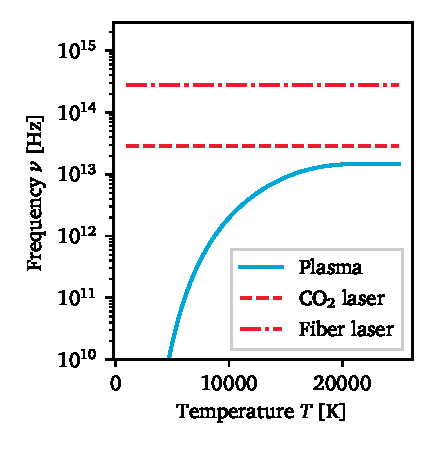
\includegraphics[]{assets/4 models/frequency_comparison}
                \caption{Comparison of plasma and laser frequencies}
                \label{fig:coulomb_freq}
            \end{subfigure}
            \hfill
            \begin{subfigure}[t]{2.9in}
                \centering
                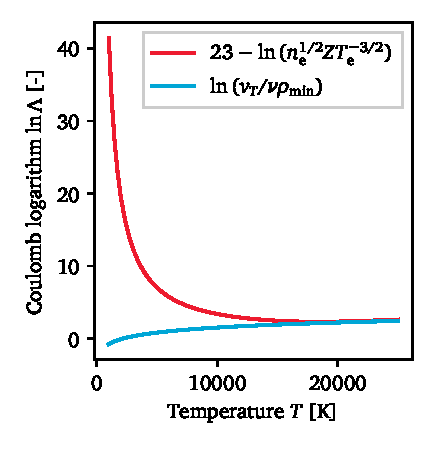
\includegraphics[]{assets/4 models/coulombLog}
                \caption{Comparison of computation methods}
                \label{fig:coulomb_coulomb}
            \end{subfigure}
            \caption{Calculation of the Coulomb logarithm, \qty{10}{bar}}
            \label{fig:coulomb}
        \end{figure}

        With values for the Coulomb logarithm and the plasma frequency, \autoref{eq:ib_absorption} can be evaluated. \autoref{fig:ib_coeff} plots the IB absorption coefficient for a range of temperatures and pressures. The point of peak absorption appears around the \qty{20000}{K} mark, with a sharp rise in peak absorption coefficient with increasing pressure. This is expected as $\alpha$ is proportional to $n_\mathrm{e}^2$ on the first order, which increases with pressure. The occurrence of peak absorption appears to shift to greater temperatures as pressure increases.

        \begin{figure}[h]
            \centering
            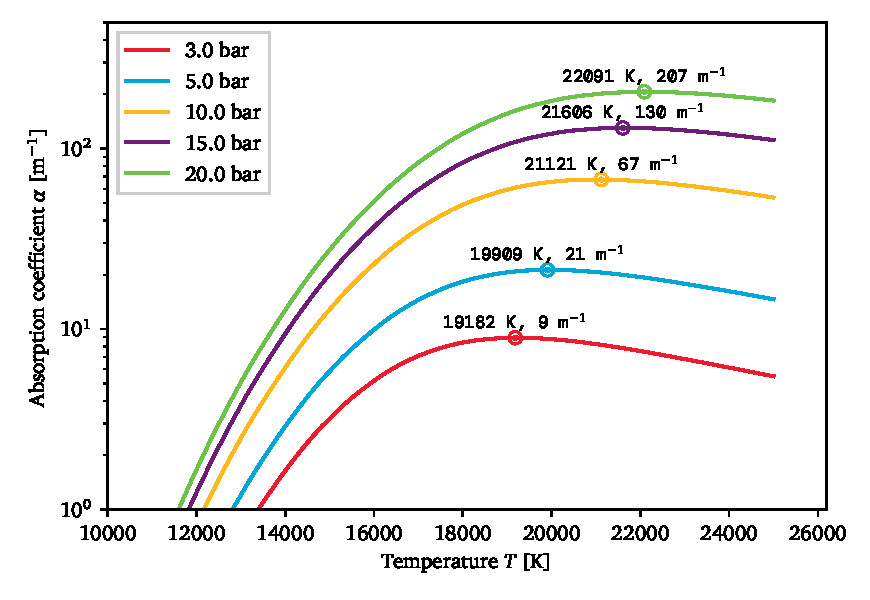
\includegraphics[]{assets/4 models/absorption}
            \caption{Inverse bremsstrahlung absorption coefficient of Argon at various pressures, \qty{1070}{nm} radiation}
            \label{fig:ib_coeff}
        \end{figure}

        The temperature of peak absorption is of interest, as it correlates to the peak temperature of the LSP (\textcite{keeferLaserSustainedPlasmas1989}). This absorption model thus suggests that a peak temperature of around \qty{20000}{K} should be expected.
    \chapter{Experiments}

    \section{V1}

        \subsection{Spark ignition}
            
            As was discussed in \textcite{duplayArgonLaserPlasmaThruster2024a}, spark ignition was not reliable enough with the available electrode system. 

        \subsection{Bringing the pulsed power down and Optical design (move to design)} \label{sec:pulse_power_down_V1}
            
            Pulsed shots at lower power levels revealed a difficulty to ignite the LSP below \qty{20}{\%} power, which corresponds to about \qty{620}{W}. This poses a problem, as the maximum CW power of the laser is significantly lower, at \qty{350}{W}. A test campaign was started in February 2024 to determine if LSP ignition in the V1 thruster was possible under this maximum CW power level.
            
            To obtain LSP ignition, a high enough laser flux is needed. With a fixed power, it is necessary to focus the laser down to the smallest area possible to get the highest flux. Quantifying the diameter of this focus was therefore the first step. 

            %Section on quantifying diameter, laser optics basics (email from thorlabs guy)

            For a multi-element system, the spot diameter must be calculated numerically with ray tracing software. WinLens 3D Basic \cite{winlens} was used here, as it is free and powerful enough for this application. The single element system was also simulated in this software to verify the calculations.

            Now that the diameter of the focus is known, two avenues are possible to improve it: a shorter focal length or a multi-lens system \cite{thorlabs}. At first, a single lens with a \qty{125}{mm} focal length (Thorlabs LA1384-C \cite{125mm lens}) was used, as it was the simpler option. During these shots, the goal was to achieve LSP ignition at or below \qty{11}{\%} pulsed power, or \qty{340}{W}. The following graph shows LSP ignition attempts at various power settings and axial lens positions. 20 pulsed laser shots were performed for each point on the graph. If at least one was successful at igniting LSP, it was recorded as such. This graph can also be interpreted as a beam profiling for LSP conditions.
            
            % Graph of 125mm lens
            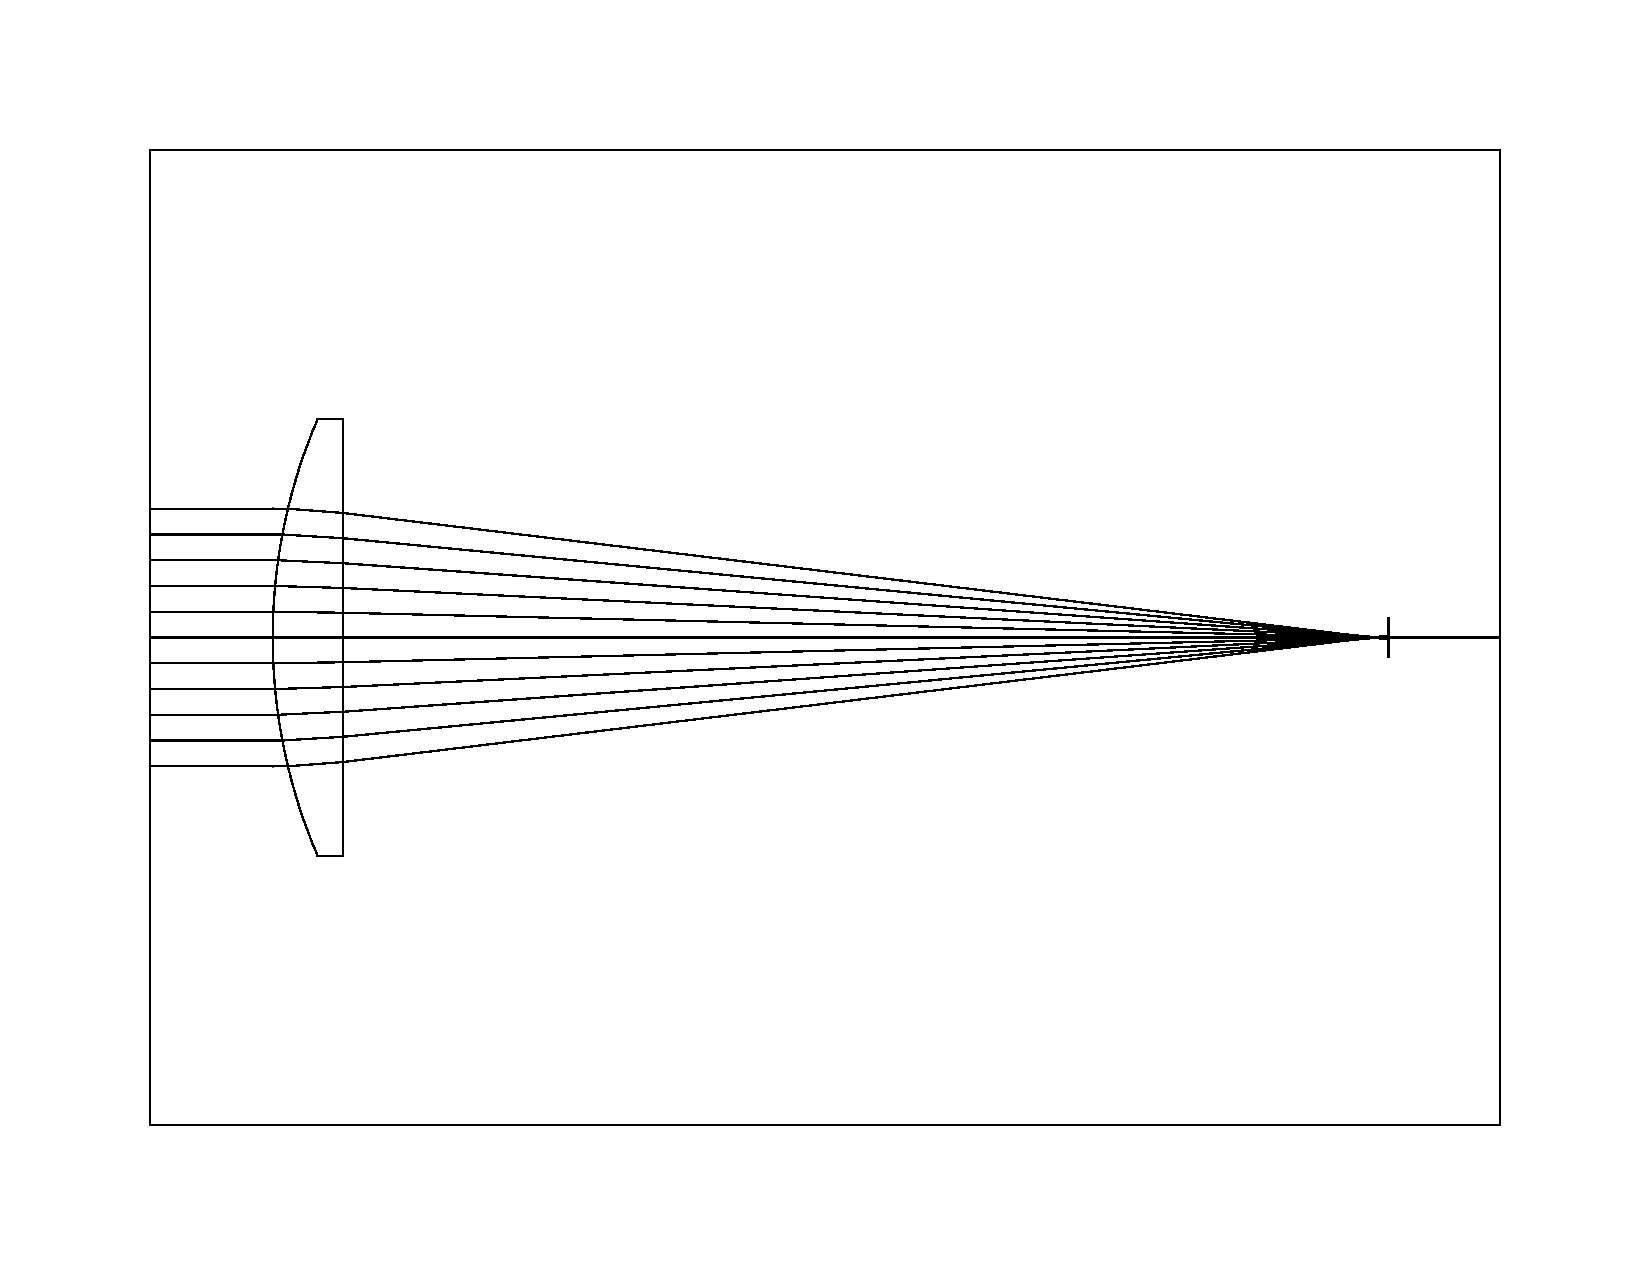
\includegraphics[width=\textwidth]{assets/5 results/125lens.pdf}

            \begin{figure}[h]
                \centering
                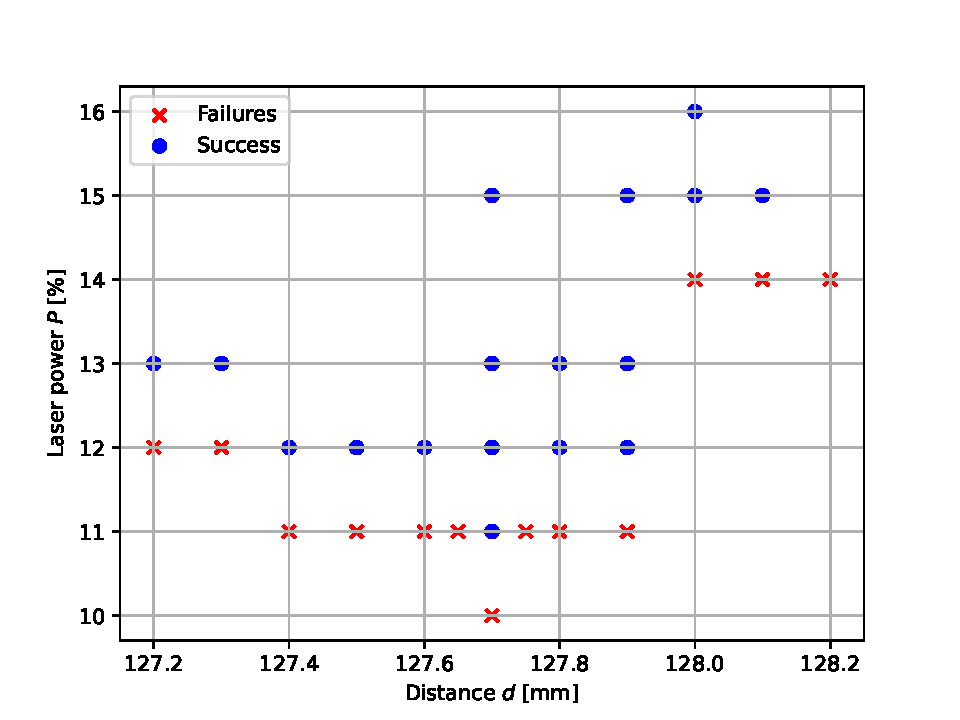
\includegraphics[width=0.75\textwidth]{assets/5 results/125mm_focus_threshold.pdf}
                \caption{125 mm focal length lens}
            \end{figure}
            
            Ignition at \qty{11}{\%} was attained once, but it was not possible to replicate this. A tighter focus was necessary to increase ignition reliability.

            % Graph of multi-lens
            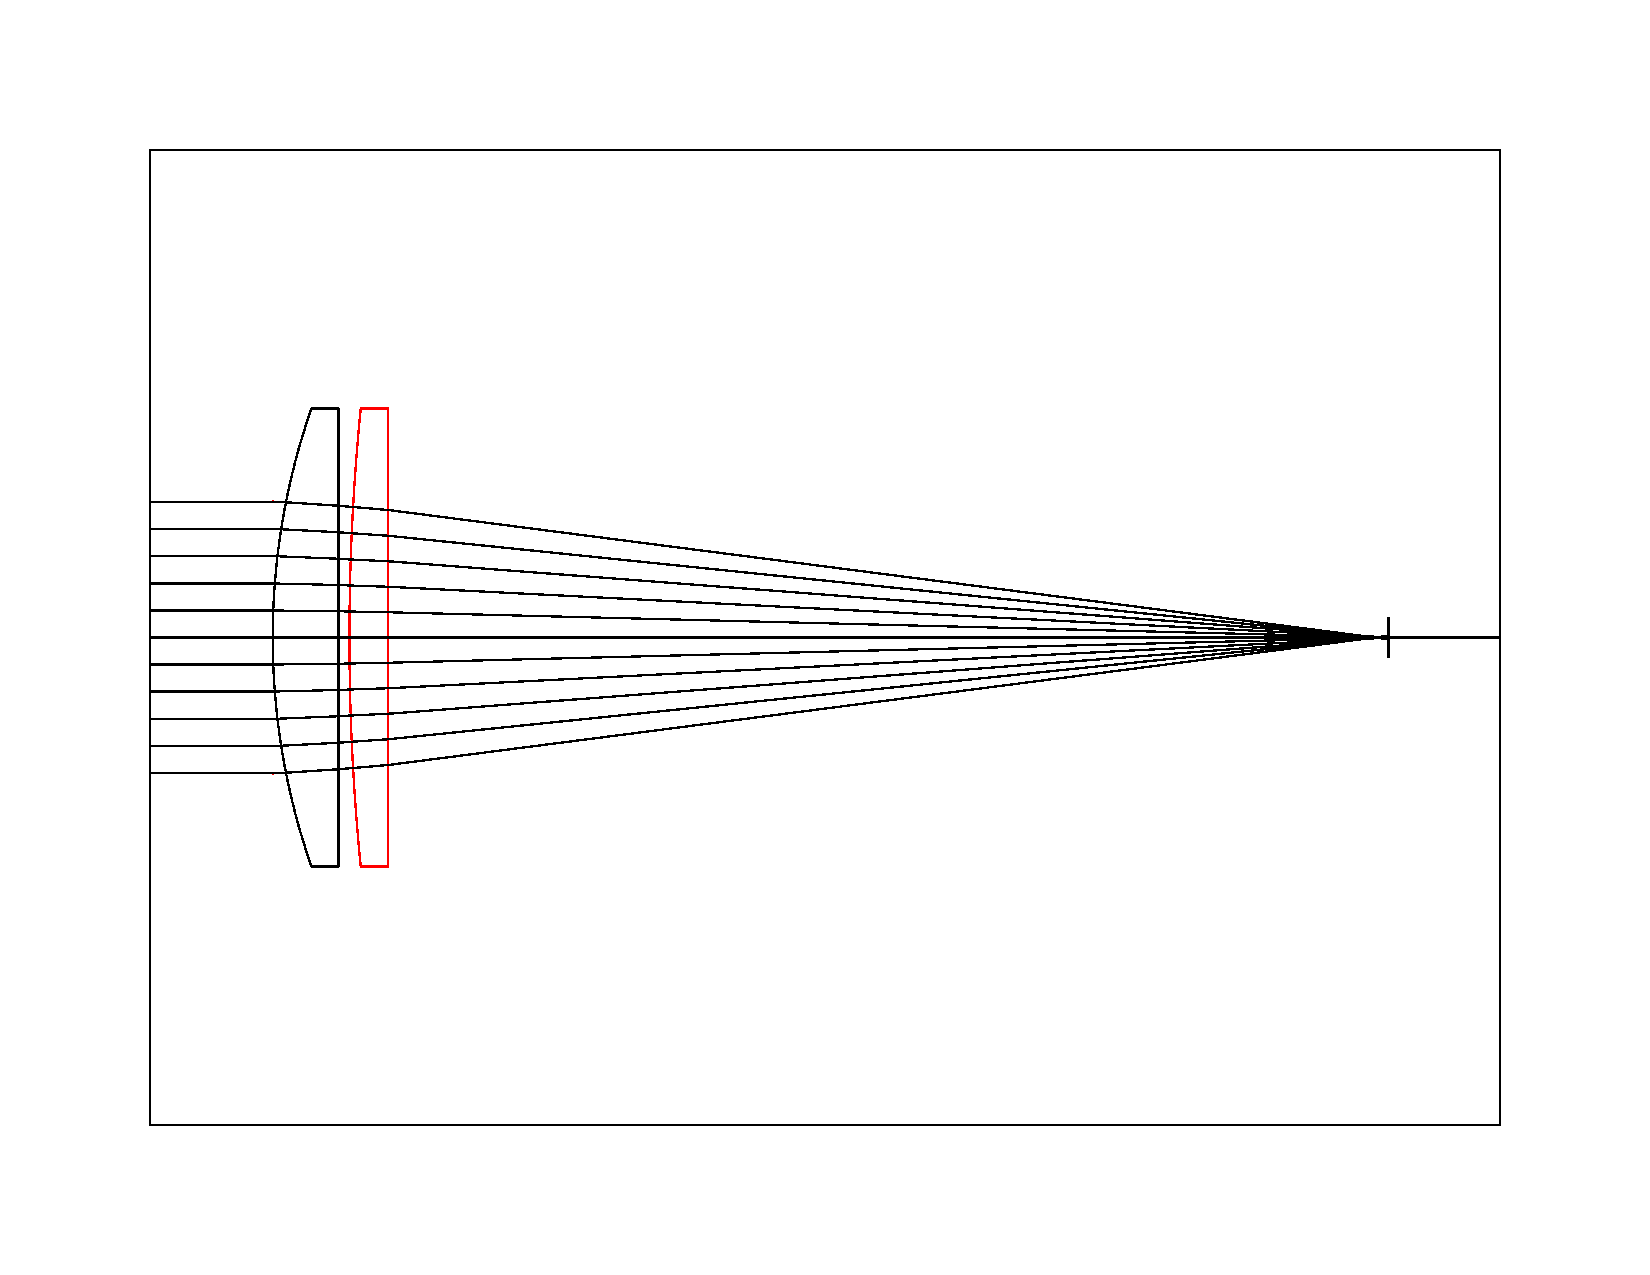
\includegraphics[width=\textwidth]{assets/5 results/500 and 150 lenses.pdf}

            \begin{figure}[h]
                \centering
                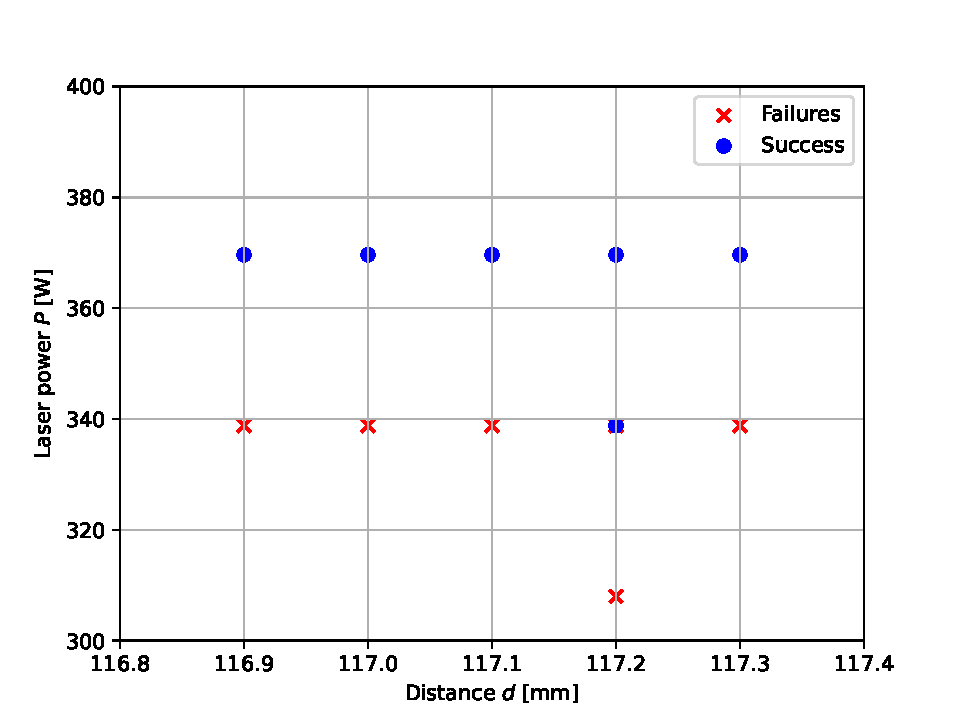
\includegraphics[width=0.75\textwidth]{assets/5 results/duallens_focus_threshold.pdf}
                \caption{Multi-lens system}
            \end{figure}

            % Section on power meter reading lower pulsed power at these low power settings, like about 200W

            The completion of these tests validated LSP generation in the CW power regime of the laser. The V2 thruster was then set up to ultimately test CW operation with flowing argon.
        
        \subsection{\ce{NO2} seeding}
            
            As the plasma emits in the ultraviolet (UV) range, it is necessary to seed with a gas that absorbs UV but not the infrared (IR) laser. \textcite{khanGasDetectionUsing2019} shows that \ce{NO2} and \ce{SO2} are two candidates. \ce{NO2} was first used as it was easy to produce in-house in significant quantities. The V1 system was set up with a vacuum pump connected to an outside air exhaust to safely vent the \ce{NO2} gas. The pump was also used to bring the pressure in the test section down to vacuum (how much?) before introducing gas.

            Control LSP shots were undertaken in pure argon. Next, 0.55 bar of \ce{NO2}, or 200 mL at STP, were introduced into the chamber. It was then pressurized with argon to 20 bar. With the spark active, LSPs were consistently generated in the seeded atmosphere and their pressure trace from the PCB transducer was recorded with the oscilloscope. This pressure rise was approximately double the one seen in pure argon; see \autoref{fig:NO2_shots_analysis}.

            The next series of LSP shots was conducted with 0.24 bar (\qty{85}{ml} at STP) of \ce{NO2} and filled to 20.2 bar of argon. Again, higher pressure rises were observed, but slightly less than the \qty{0.55}{bar} shots. The chamber was finally half evacuated to 10.17 bar and then filled back to \qty{20.15}{bar}. This should bring the partial pressure of \ce{NO2} to \qty{0.12}{bar}. Again, LSPs were consistent, with a higher pressure rise than pure argon, but less than the higher concentration \ce{NO2} shots.

            \begin{figure}[h]
                \centering
                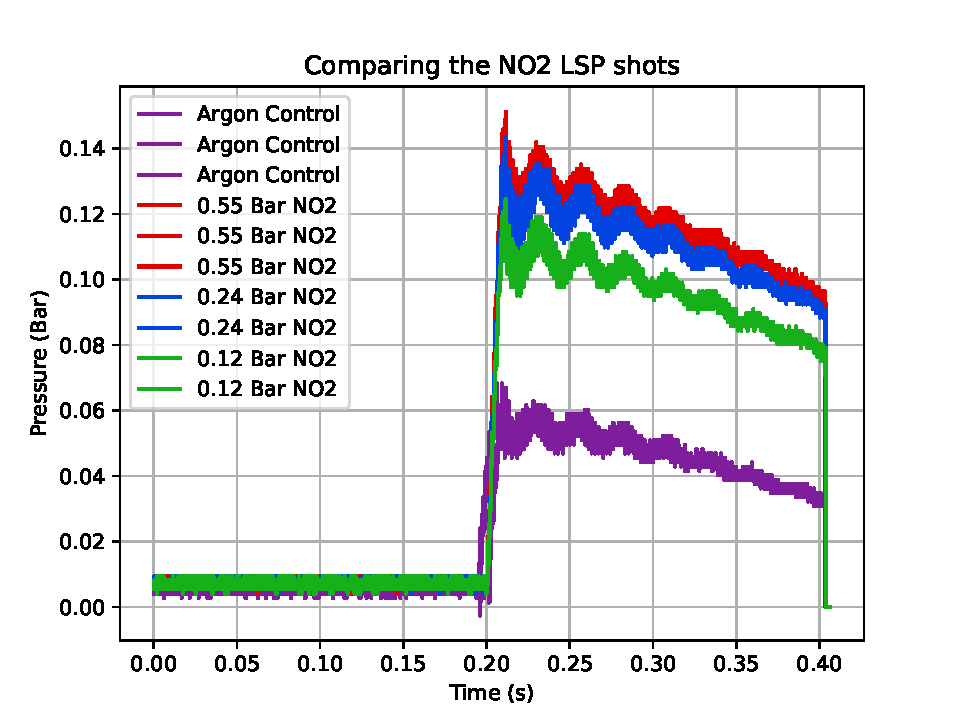
\includegraphics[width=0.75\textwidth]{assets/5 results/NO2_shots_analysis.pdf}
                \caption{NO2 LSP shots}
                \label{fig:NO2_shots_analysis}
            \end{figure}

            Indeed, with as low as (0.5\%?) of \ce{NO2} mixed with argon, nearly double the pressure rise is observed. This indicates that the working gas is absorbing twice the energy from the plasma. As the \ce{NO2} fraction is increased, there are diminishing returns to the pressure rise. This is encouraging, as not much \ce{NO2} is needed to have a great impact on the energy absorption.

    \section{V2}
        This section presents the various experiments that were conducted with the V2 thruster.
    
        \subsection{Initial LSP shots}

            \begin{figure}
                \centering
                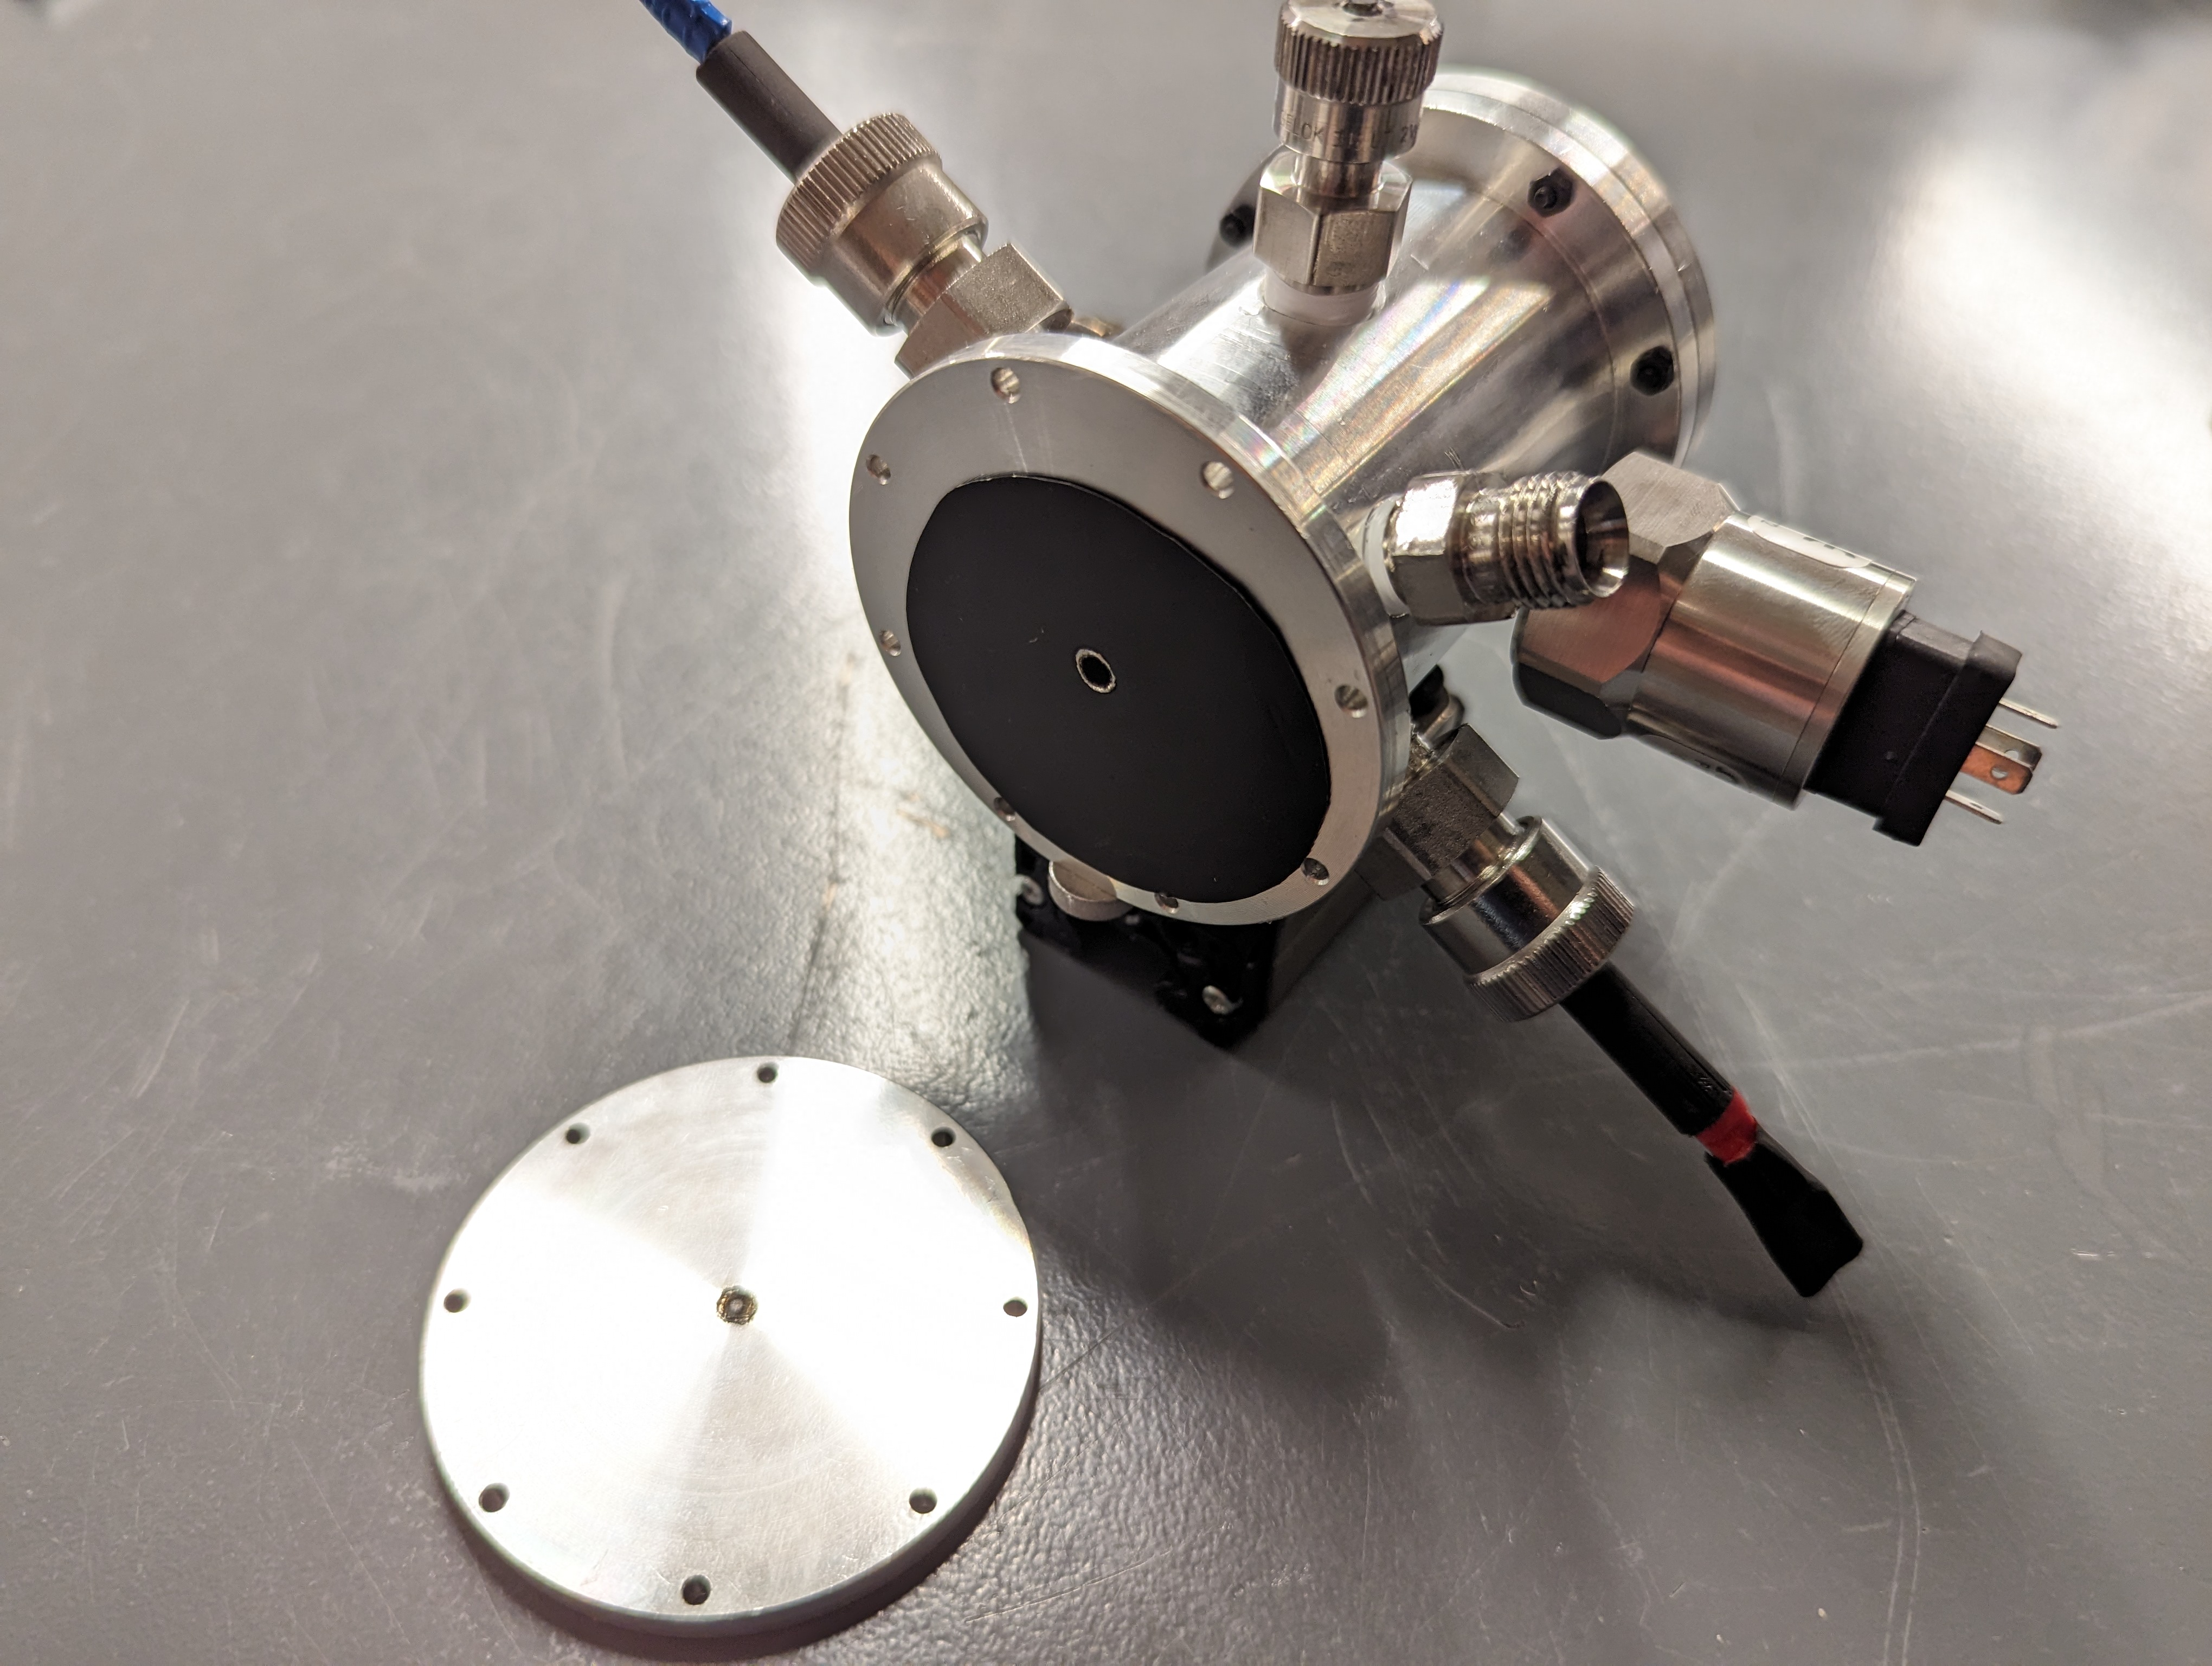
\includegraphics[width=0.75\textwidth]{assets/5 results/V2 test damage.jpg}
                \caption{Damage to the thruster after two \qty{3}{kW} laser shots}
            \end{figure}

            % Stills of first High-speed LSP video, showing expansion of LSP wave like in V1
        
        \subsection{Cold flow thrust tests}

            Cold flow tests were completed to give a baseline measurement of thrust before the hot fire test, and to validate the functioning of all data acquisition systems.
            
            % thrust vs pressure graph

        \subsection{Bringing the pulsed power down, again}
            
            To prevent the damage to the thruster seen previously, a rear window mount was manufactured. This allows the laser energy that is not absorbed to pass freely through the apparatus, also enabling power meter measurements. The following figures present the LSP ignition attempts with focus distance, similarly to the graphs presented in \autoref{sec:pulse_power_down_V1}. 
 

            

        




    \chapter{Conclusion and further work}
    Already identified as an alternative to chemical propulsion in the 1970s, laser-thermal propulsion promises the high specific impulse and thrust necessary to unlock rapid transit in the solar system. Whether this promise can be achieved in practice and at scale is however yet to be seen. McGill University's Interstellar Flight Experimental Research Group hopes to revive practical research on LSP for propulsion applications, by attempting to replicate and move beyond some of the work done in the late 20\textsuperscript{th} century with the fiber-optic lasers considered for use in other directed-energy propulsion concepts such as interstellar lightsails and laser-electric propulsion. By contrast with more recent LSP research which focused on non-propulsion applications, this project aimed to study the thermal, heat deposition, and thrust characteristics of LSP.

    A brief review of LTP and LSP literature was provided. DEP and LTP concepts were discussed, including their advantages and drawbacks. Research on LSP was summarized, starting with the physics of inverse bremsstrahlung (i.e., the physical mechanism powering LSP) and moving on the models and observations made through an intense period of research between 1970 and 1990. Researchers at the time were considering the use of \ce{CO_2} lasers emitting \qty{10.6}{\um} radiation, and the implications of a switch to \num{1.06}-\unit{\um} fiber-optic lasers were mentioned: while the range of these lasers is an order of magnitude greater, the lower IB absorption coefficient at this wavelength mandates higher laser power and/or pressure to sustain LSP. The design of past LSP facilities was briefly reviewed to provide context for the design choices made in creating such a facility at McGill, for the purposes of studying heat deposition and resulting thrust characteristics of argon LSP.

    The design process of the LTP thruster laboratory model was then reported in detail. The system's design was driven in large part by the constraints set by the laser available for this experiment, capable of emitting \num{3}-\unit{kW} pulses, but only for \qty{10}{ms}. The reasoning behind the decision to retrofit existing apparatus instead of opting for a clean-sheet design was discussed at length: given the many practical uncertainties surrounding the system, and the short timeline available for this project, the retrofit of a perhaps unoptimized test section was deemed preferable to inform the future design of a dedicated thruster model. This came at the cost of hindering thrust experiments, but this tradeoff paid off with the lessons learned in designing and rapidly testing an ignition system, developing diagnostic methodologies, and actually performing LSP experiments.

    Some modelling work was performed as part of this thesis, mainly to gain an understanding of the physics involved in inverse bremsstrahlung and the relevant parameters driving laser-sustained plasma. Namely, chamber pressure is a key parameter of any thermal propulsion system, with high pressures providing greater thrust. In LTP, higher pressures are also beneficial to improve LSP absorption properties. Predicting peak absorption (with respect to temperature) is also helpful to estimate the maximum temperature reached in the LSP, as it has been found to be correlated. \added{A simple model for LSP sizing prediction based on deposited laser energy was discussed, yielding temperature and size estimates on the same order as reported in literature and observed in experiment, respectively. The effects of heat deposition in the test section are also modelled, providing the means to estimate the heat deposition efficiency of LSP from experimental measurements. The modelling effort ends with an analysis of the expected performance of an LTP thruster model, suggesting that a dedicated thruster prototype should exhibit significant changes in thrust and exhaust velocity when powered by a laser---as long as the mass-flow rate is lower than \qty{1}{g.s^{-1}}.}

    Finally, the first results of a series of experiments were reported. Preliminary ignition tests quickly revealed the challenges posed by spark ignition. The use of such a system when constrained by a short laser pulse requires careful design to consistently align the laser focus and the spark. Successful LSP ignition using this system was difficult, but was achieved a few times, enough to build a small dataset on the laser absorption ability of LSP, which was observed to range from 70 to 90\%. Initial estimates on the absorption coefficient, derived from the absorption data and high-speed footage, appear to agree with this study's modelling, although a more systematic absorption study would be needed to confirm this. For other experiments, wire ignition was found to be far more reliable than spark ignition and allowed the replication of power threshold studies done in other LSP literature, finding that this ignition system provides a competitively low power threshold without the need of high precision optics. Spectral data acquired during these experiments should theoretically provide a measure of peak plasma temperature, but there appears to be methodology and/or processing issues to be resolved to provide a realistic temperature estimate. Flowing experiments were performed to explore the impact of incoming flow on LSP properties, but the feed system limitations only allowed for a cursory exploration.
    
    The recorded pressure change during and shortly after the LSP provided an insight into the heat deposition into the gas volume by the LSP. This ability will be crucial in a fully realized LTP system: to provide specific impulse on the order of \qty{3000}{s} yet high thrust, the LSP is meant to heat the surrounding propellant, and not be exhausted by itself (which would result in higher specific impulse but only for low thrust). The experimental data suggests a low heat-deposition efficiency of around 15\%, relative to the laser power incident on the LSP. Combined with the measured absorption, this builds an overall picture of the major loss factors involved in LSP: incomplete laser absorption and heat radiated to the walls or outside the test section appear to be responsible for 20\% and 65\% of the energy losses, respectively. This provides a baseline on efficiency that can now be improved on with a variety of strategies suggested in the LTP literature. The peculiar shape of the pressure profile, with its local maximum and minimum, should be the subject of further study.

    The objectives set for this project, to build an argon LTP thruster model, may not have been entirely met. Issues encountered with the unoptimized test section and its impact on thrust measurement meant that meaningful thrust experiments could not be performed. However, a method to determine heat deposition into the working gas was developed based on the pressure change of the test section, providing a baseline on heat-deposition efficiency, which can be used to design the next iteration of an LTP thruster at McGill University. In this regard, the project is successful in initiating a new experimental research effort on LTP at the IFERG, and the questions and issues raised across various aspects of this project could motivate several new, more targeted studies.

    \section{Further work}
        As this thesis project's \emph{raison d'être} was to lay the groundwork for experimental research on LSP and LTP at McGill, there are many opportunities for further work. A selection of such opportunities is given below.

        \paragraph{Optimization of the test section} Although the retrofit of the cavitation experiment's test section enabled rapid experimentation, its non-optimal design posed several challenges, some of which were already discussed in \autoref{sec:design_testSection}. The test section mass was particularly problematic for thrust experiments. Further research on LSP and LTP will be limited without the development of a new LSP generator or prototype thruster optimized for this project. Such optimizations would include:
        \begin{itemize}
            \item Opting for a lighter material for the pressure vessel, likely aluminum, to minimize weight
            \item Reducing the overall length and diameter of the vessel. This would both provide more flexibility in terms of beam geometry, allowing the use of shorter lenses or placing the laser focus at different locations in the chamber, to potentially optimize the LSP location relative to the nozzle. Smaller dimensions would also reduce the overall weight\added{ and result in a greater measured change in temperature and pressure, as implied by \autoref{eq:heatdep}}.
            \item Smaller observation windows. Although the current side windows offer excellent visibility throughout the length of the test section, their slender geometry and length mandated the use of heavy steel mounting clamps. Opting for lighter, smaller round windows bolted directly into the pressure vessel's body may be sufficient.
        \end{itemize}
        Such improvements would greatly facilitate the development of an appropriate thrust stand and provide greater beam-shaping flexibility without compromising on laser absorption measurements.

        \paragraph{Improved spark-ignition system} As discussed in \autoref{sec:ignitiontest}, the original spark-igniter design for this study proved difficult to work with, as the large spark gap and side-by-side electrodes created inconsistent arc paths that would rarely intersect with the laser beam path. Although good results were obtained with wire ignition, spark ignition is still thought to be optimal for future experiments, as its advantages over wire ignition would be worth the additional development efforts. As a reminder, they are as follows:
        \begin{itemize}
            \item An uninterrupted laser beam path allows determining the absorbed laser power and the absorption coefficient. It also does not impede the downstream growth of the LSP.
            \item Sparks can be generated at will without consuming material between each test. Several experiments could potentially be done in quick succession without re-aligning optics or replacing the ignition wire.
        \end{itemize}
        In order to improve spark consistency and ignition reliability, several improvements could be made to both the spark-plug design and how it integrates in the test section:
        \begin{itemize}
            \item The electrodes should be in a co-axial configuration, as was done for several LSP experiments in the literature (\textcite{luCharacteristicDiagnosticsLaserStabilized2022, zimakovInteractionNearIRLaser2016,matsuiGeneratingConditionsArgon2019}). This may improve the consistency of the arc path and would enable precise mechanical control of electrode distance more easily than with side-by-side electrodes.
            \item To accommodate for such an electrode arrangement, the test section should be modified with instrumentation ports along the opposite wall of the cylinder. Each port should ideally be precisely matched with another port facing it.
            \item Electrode tip distance should be reduced down to about a millimeter to favor arcing even at \qty{20}{bar} and to constraint possible arc paths to those intersecting with the laser focus. Ideally, this gap should be adjustable in order to adapt the electrode distance based on the test pressure.
            \item Discussions with researchers experienced with spark igniters suggested that a sharp tipped electrode paired with a rounded electrode gave better results.
        \end{itemize}

        \paragraph{Specific impulse measurement} One of the ultimate goals of the LTP project at McGill University is to demonstrate the feasibility of the concept and show that a specific impulse of \qtyrange{1000}{3000}{s} is possible under the right conditions. While the roadmap to this sort of performance is long and would involve a switch to hydrogen as a working gas, the experiment should be set-up such that mass-flow rates can be controlled and/or measured, enabling the calculation of exhaust velocity when combined with thrust data. This can be done using a mass flowmeter or by controlling mass flow by operating the facility in a double-choked configuration (choked at inlet and exhaust nozzle).

        \paragraph{Absorption measurements in flowing conditions} The nozzles used in this study could be easily fabricated and swapped on the test section but made it impossible to acquire an accurate measure of the laser power transmitted through the LSP and out of the test section, as the orifice size was significantly smaller than the laser beam. Designing a nozzle module that allows such a measurement would permit the study of the effect of flow on laser absorption. Poor laser absorption is one of the main efficiency loss mechanisms for an LTP thruster, so being able to measure it in flowing conditions would be valuable. This can be done either by using a regular laser window mount with an off-axis nozzle, or by designing an annular nozzle around the laser window (whether this option is worth the considerable design effort is debatable).

        \paragraph{Additional spectrometry and thermal imaging} As discussed in \autoref{sec:results_spectroscopy}, there is much room to improve this experiment's spectroscopy methodologies. The spectrometer's fiber termination should be equipped with a collimator to sample precise points in the LSP, which should improve the spectral data for temperature estimation with the Boltzmann plot method. Once this is corrected, the collimator could be mounted on opto-mechanical stages to precisely position it relative to the LSP, enabling the construction of temperature maps of the LSP, which could be compared to axisymmetric numerical models currently in development at McGill (\textcite{baoTwoDimensionalSimulationLasera}). In addition to spectroscopy, infrared thermal imaging could potentially be used to study the change in temperature of the cooler surrounding gas, providing additional data on the effective heat deposition from the LSP.
    
    \clearpage
    \defbibnote{bibmark}{\markright{}}
    \printbibliography[
        heading=bibintoc,
        title={References},
        block=ragged,
        prenote=bibmark
        ]
    \newpage

    \appendix
    \newcommand{\footeronly}{\thispagestyle{fancy}\markboth{}{}}
    

\end{document}